\documentclass[12pt]{extarticle}
\usepackage[paperwidth=18in,paperheight=8.5in]{geometry}
\usepackage{amsmath}
\usepackage{hyperref}
\usepackage{multirow}
\usepackage{pdfpages}
\usepackage[utf8]{inputenc}
\title{Kaon mixing: chiral and continuum extrapolations}
\author{R Mukherjee}
\date{\today}
\begin{document}
\maketitle
\tableofcontents
\clearpage
\begin{figure}
\centering
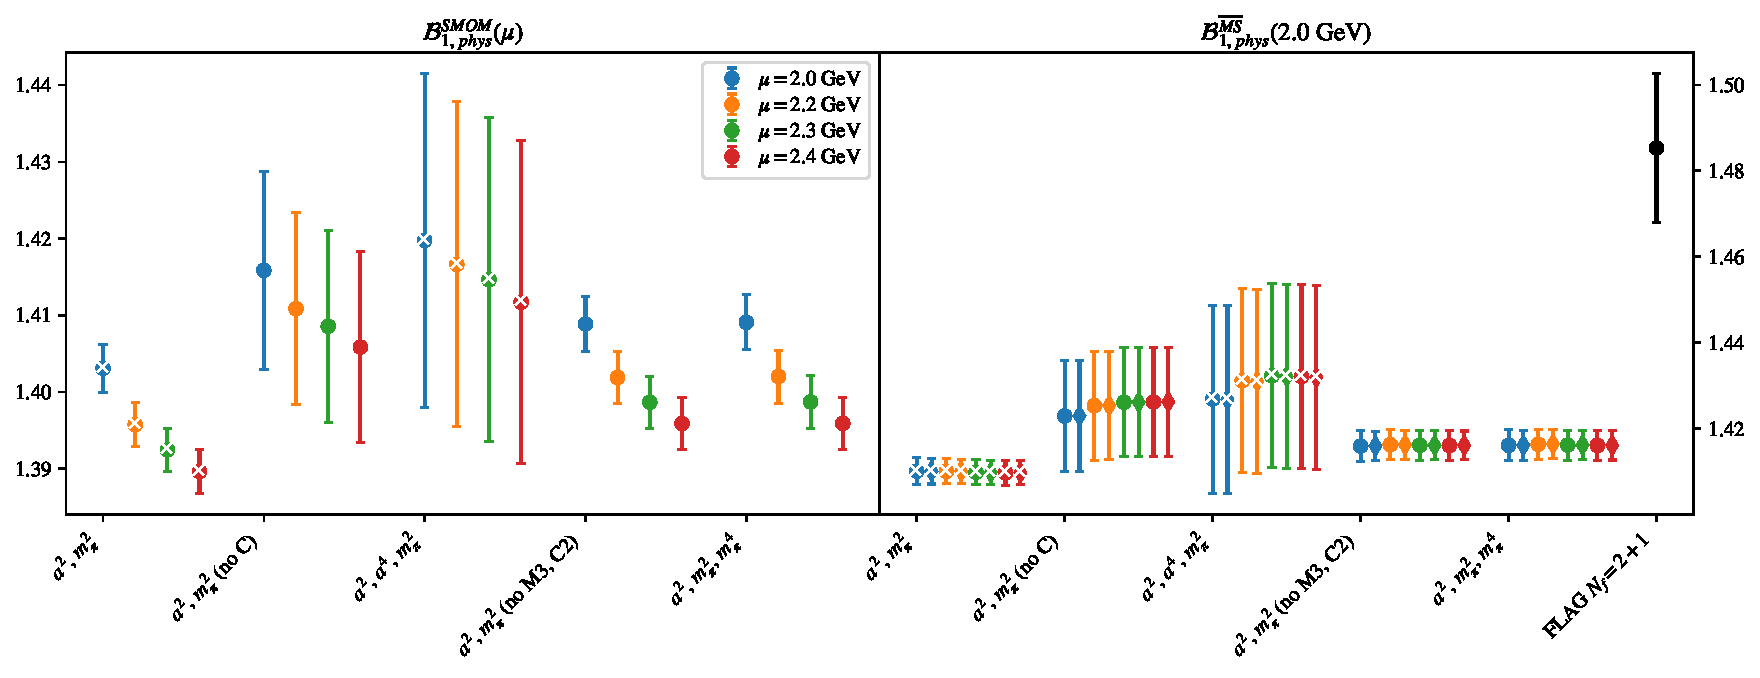
\includegraphics[page=1, width=1.1\textwidth]{VVpAA/SUSY/fit_summary_bag.pdf}
\caption{$\mathcal{B}_{1}$\\(left) $\mathcal{B}_{phys}$ in RI/SMOM scheme from fit variations (fits with $p$-value $<0.05$ marked with ``$\times$"). \\(right) $\mathcal{B}_{phys}$ in $\overline{MS}$ computed using $\mathcal{B}^{\overline{MS}} = R^{\overline{MS}\leftarrow SMOM}(2.0)\sigma_{npt}(2.0,\mu) \mathcal{B}^{SMOM}(\mu)$.}
\end{figure}
\clearpage
\begin{figure}
\centering
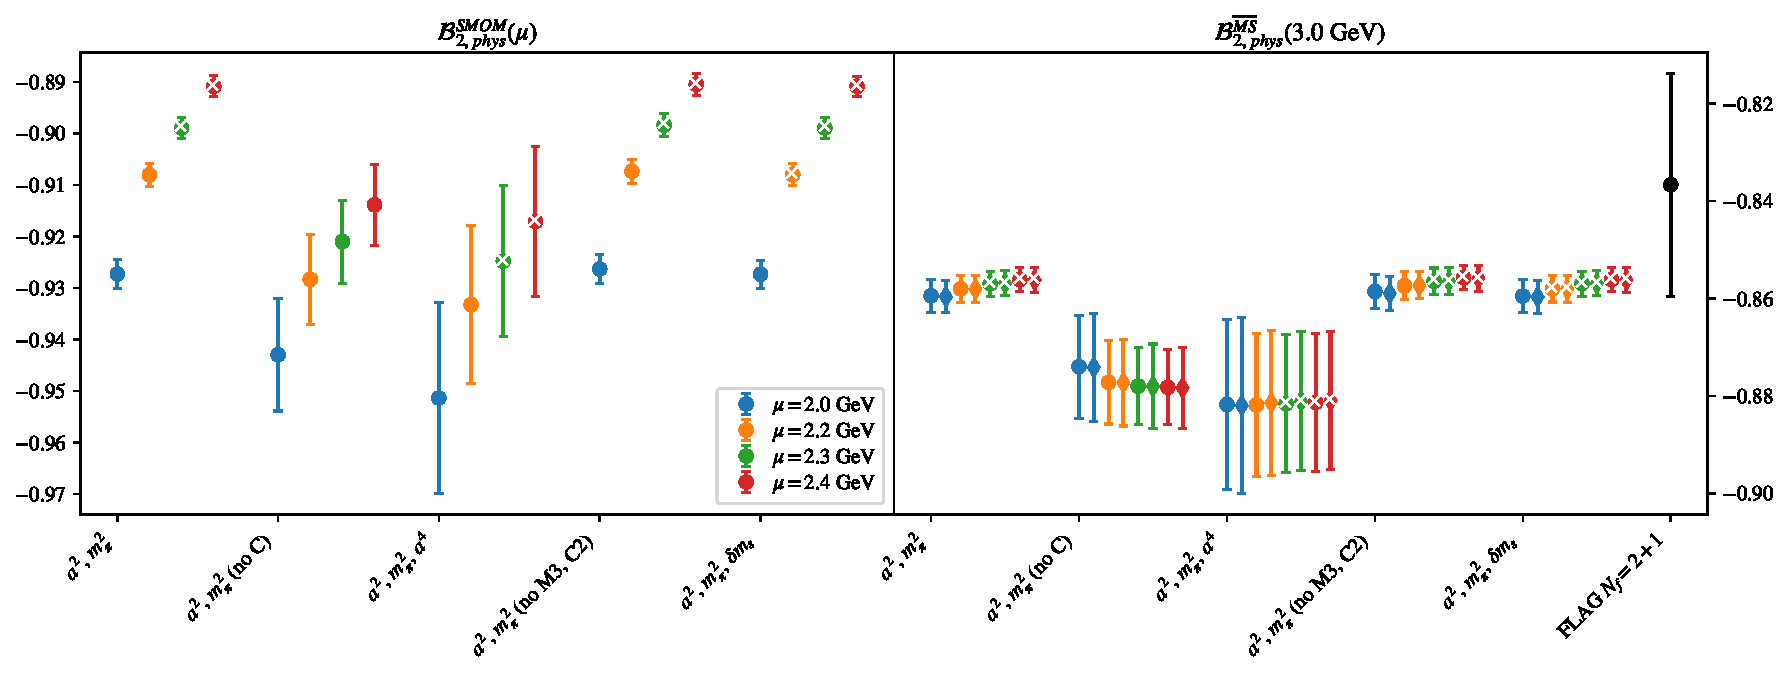
\includegraphics[page=1, width=1.1\textwidth]{VVmAA/SUSY/fit_summary_bag.pdf}
\caption{$\mathcal{B}_{2}$\\(left) $\mathcal{B}_{phys}$ in RI/SMOM scheme from fit variations (fits with $p$-value $<0.05$ marked with ``$\times$"). \\(right) $\mathcal{B}_{phys}$ in $\overline{MS}$ computed using $\mathcal{B}^{\overline{MS}} = R^{\overline{MS}\leftarrow SMOM}(3.0)\sigma_{npt}(3.0,\mu) \mathcal{B}^{SMOM}(\mu)$.}
\end{figure}
\clearpage
\begin{figure}
\centering
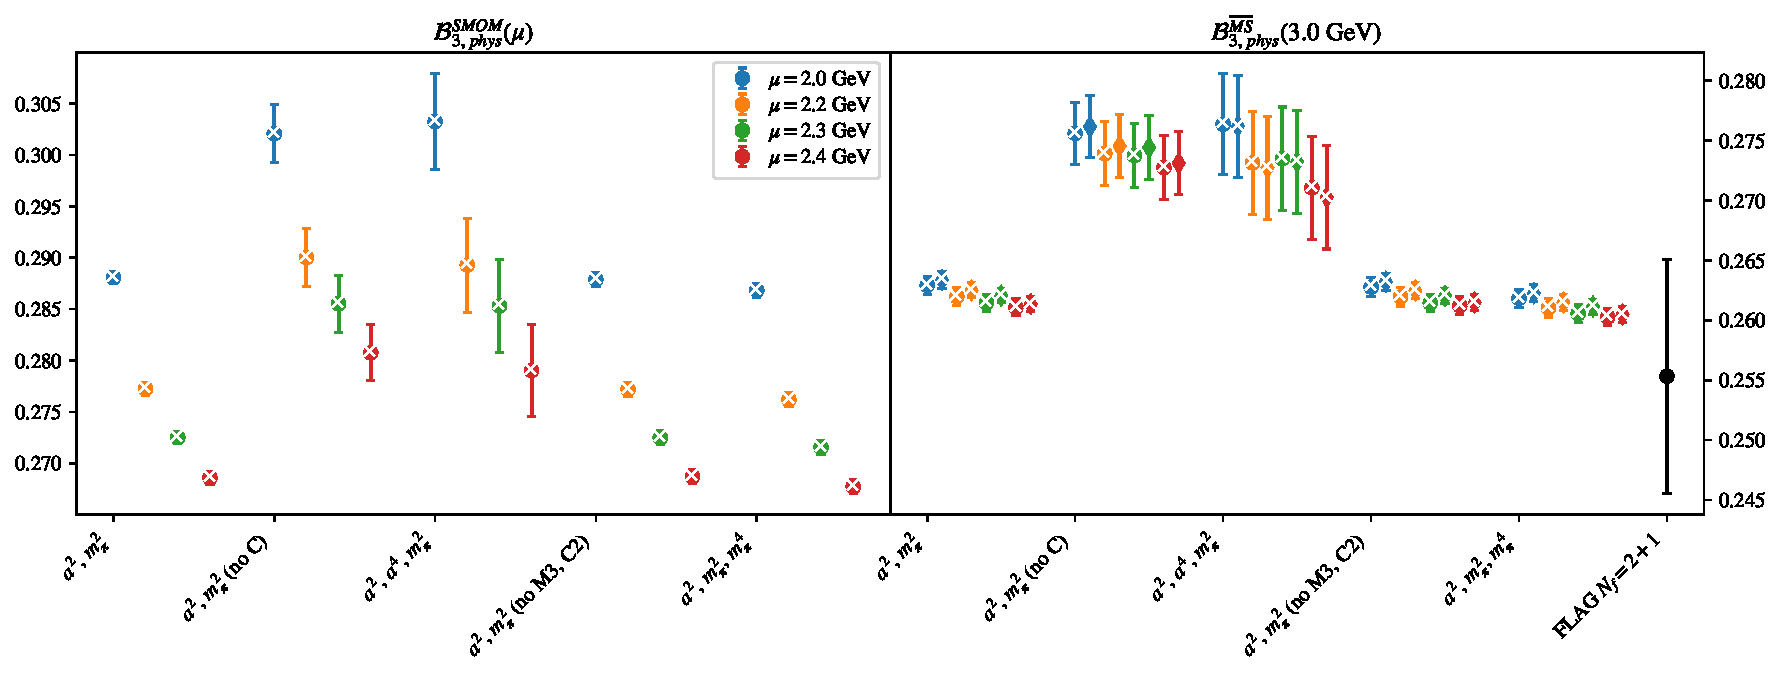
\includegraphics[page=1, width=1.1\textwidth]{SSmPP/SUSY/fit_summary_bag.pdf}
\caption{$\mathcal{B}_{3}$\\(left) $\mathcal{B}_{phys}$ in RI/SMOM scheme from fit variations (fits with $p$-value $<0.05$ marked with ``$\times$"). \\(right) $\mathcal{B}_{phys}$ in $\overline{MS}$ computed using $\mathcal{B}^{\overline{MS}} = R^{\overline{MS}\leftarrow SMOM}(3.0)\sigma_{npt}(3.0,\mu) \mathcal{B}^{SMOM}(\mu)$.}
\end{figure}
\clearpage
\begin{figure}
\centering
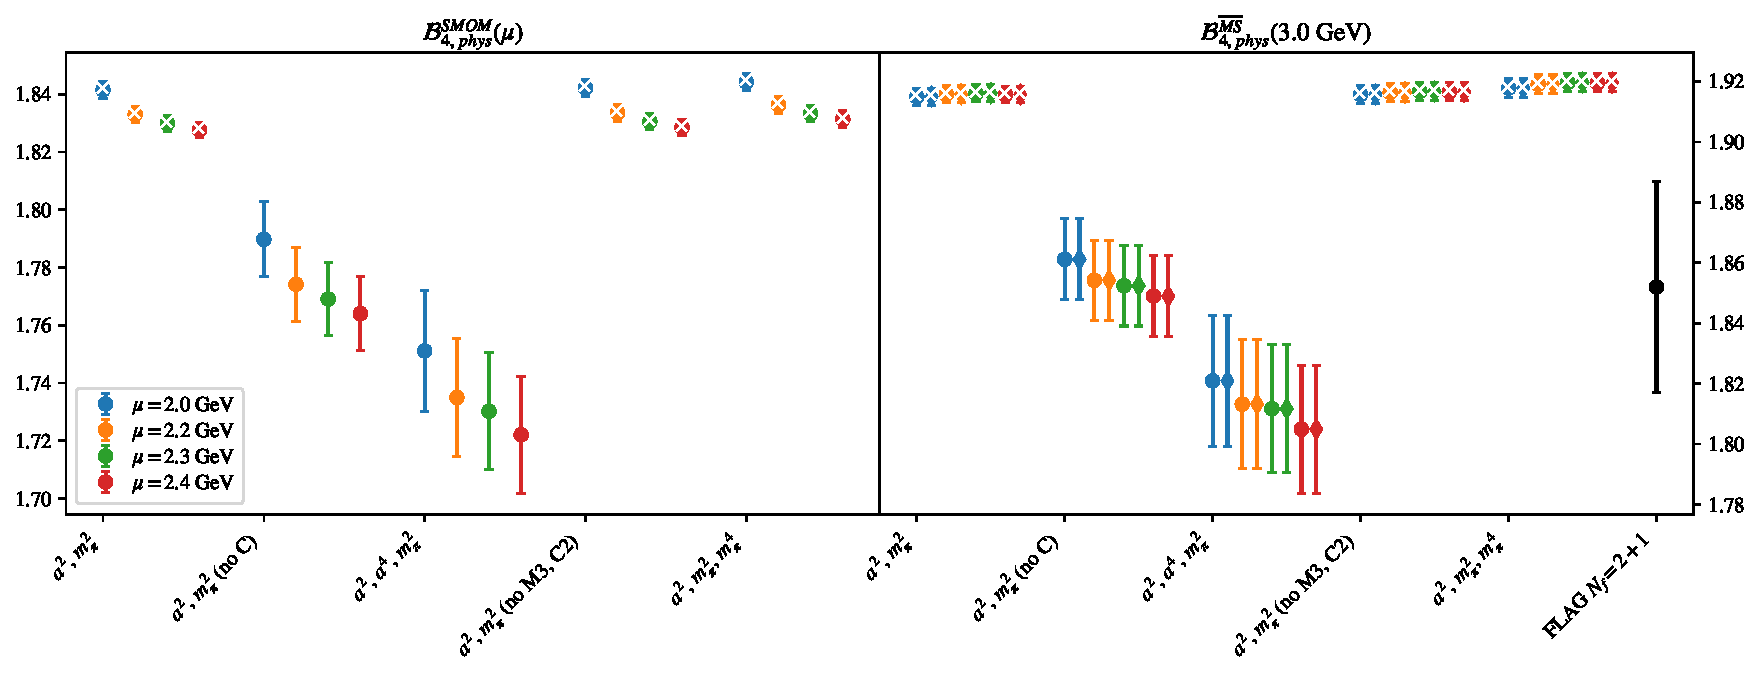
\includegraphics[page=1, width=1.1\textwidth]{SSpPP/SUSY/fit_summary_bag.pdf}
\caption{$\mathcal{B}_{4}$\\(left) $\mathcal{B}_{phys}$ in RI/SMOM scheme from fit variations (fits with $p$-value $<0.05$ marked with ``$\times$"). \\(right) $\mathcal{B}_{phys}$ in $\overline{MS}$ computed using $\mathcal{B}^{\overline{MS}} = R^{\overline{MS}\leftarrow SMOM}(3.0)\sigma_{npt}(3.0,\mu) \mathcal{B}^{SMOM}(\mu)$.}
\end{figure}
\clearpage
\begin{figure}
\centering
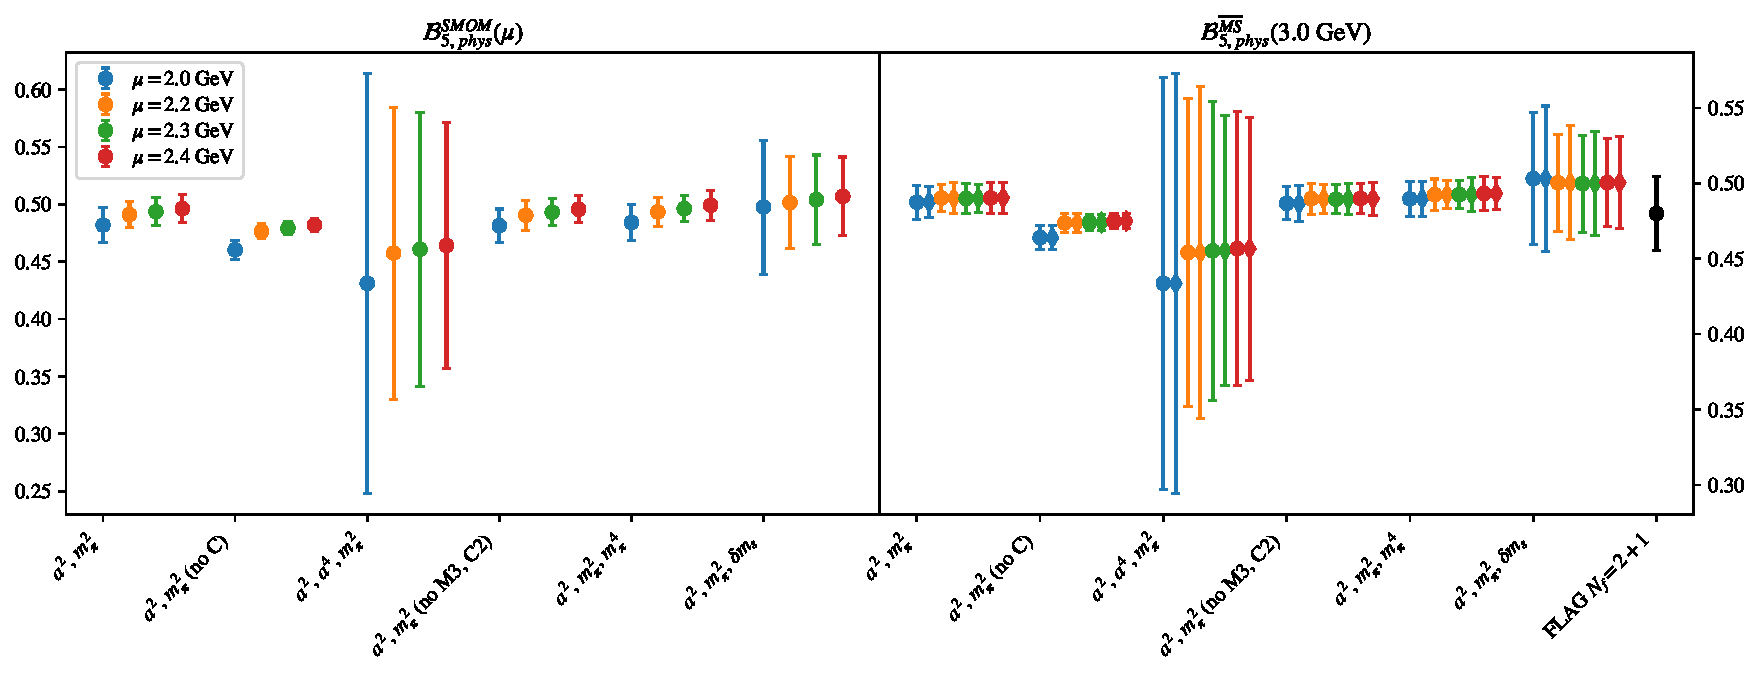
\includegraphics[page=1, width=1.1\textwidth]{TT/SUSY/fit_summary_bag.pdf}
\caption{$\mathcal{B}_{5}$\\(left) $\mathcal{B}_{phys}$ in RI/SMOM scheme from fit variations (fits with $p$-value $<0.05$ marked with ``$\times$"). \\(right) $\mathcal{B}_{phys}$ in $\overline{MS}$ computed using $\mathcal{B}^{\overline{MS}} = R^{\overline{MS}\leftarrow SMOM}(3.0)\sigma_{npt}(3.0,\mu) \mathcal{B}^{SMOM}(\mu)$.}
\end{figure}
\clearpage
\section{$\mathcal{B}_1$}
\begin{table}[h!]
\begin{center}
\begin{tabular}{|c|c|c|c|c|c|c|}
\hline
$\mu$ (GeV) & $a^2$, $m_\pi^2$& $a^2$, $m_\pi^2$ (no C)& $a^2$, $m_\pi^2$, $a^4$& $a^2$, $m_\pi^2$ (no M3, C2)& $a^2$, $m_\pi^2$, $m_\pi^4$& $a^2$, $m_\pi^2$, $\delta m_s$\\
\hline
2.0& \hyperlink{VVpAA/SUSY/bag_a2m2_20.pdf.1}{\textbf{1.4024(29)}: 2.347 (0.039)} & \hyperlink{VVpAA/SUSY/bag_a2m2noC_20.pdf.1}{\textbf{1.436(12)}: 0.223 (0.8)} & \hyperlink{VVpAA/SUSY/bag_a2a4m2_20.pdf.1}{\textbf{1.457(21)}: 1.329 (0.256)} & \hyperlink{VVpAA/SUSY/bag_a2m2mcut_20.pdf.1}{\textbf{1.4062(33)}: 2.004 (0.111)} & \hyperlink{VVpAA/SUSY/bag_a2m2m4_20.pdf.1}{\textbf{1.4051(33)}: 2.362 (0.051)} & \hyperlink{VVpAA/SUSY/bag_a2m2delm_20.pdf.1}{\textbf{1.4029(29)}: 0.738 (0.566)}\\
2.2& \hyperlink{VVpAA/SUSY/bag_a2m2_22.pdf.1}{\textbf{1.3949(29)}: 2.793 (0.016)} & \hyperlink{VVpAA/SUSY/bag_a2m2noC_22.pdf.1}{\textbf{1.431(12)}: 0.353 (0.703)} & \hyperlink{VVpAA/SUSY/bag_a2a4m2_22.pdf.1}{\textbf{1.453(21)}: 1.664 (0.155)} & \hyperlink{VVpAA/SUSY/bag_a2m2mcut_22.pdf.1}{\textbf{1.3989(32)}: 2.36 (0.069)} & \hyperlink{VVpAA/SUSY/bag_a2m2m4_22.pdf.1}{\textbf{1.3978(33)}: 2.785 (0.025)} & \hyperlink{VVpAA/SUSY/bag_a2m2delm_22.pdf.1}{\textbf{1.3954(29)}: 0.922 (0.45)}\\
2.3& \hyperlink{VVpAA/SUSY/bag_a2m2_23.pdf.1}{\textbf{1.3916(28)}: 2.928 (0.012)} & \hyperlink{VVpAA/SUSY/bag_a2m2noC_23.pdf.1}{\textbf{1.428(12)}: 0.357 (0.7)} & \hyperlink{VVpAA/SUSY/bag_a2a4m2_23.pdf.1}{\textbf{1.451(21)}: 1.727 (0.141)} & \hyperlink{VVpAA/SUSY/bag_a2m2mcut_23.pdf.1}{\textbf{1.3958(32)}: 2.481 (0.059)} & \hyperlink{VVpAA/SUSY/bag_a2m2m4_23.pdf.1}{\textbf{1.3945(33)}: 2.854 (0.022)} & \hyperlink{VVpAA/SUSY/bag_a2m2delm_23.pdf.1}{\textbf{1.3921(29)}: 0.949 (0.434)}\\
2.4& \hyperlink{VVpAA/SUSY/bag_a2m2_24.pdf.1}{\textbf{1.3887(28)}: 2.989 (0.011)} & \hyperlink{VVpAA/SUSY/bag_a2m2noC_24.pdf.1}{\textbf{1.425(12)}: 0.371 (0.69)} & \hyperlink{VVpAA/SUSY/bag_a2a4m2_24.pdf.1}{\textbf{1.448(21)}: 1.801 (0.126)} & \hyperlink{VVpAA/SUSY/bag_a2m2mcut_24.pdf.1}{\textbf{1.3929(32)}: 2.515 (0.056)} & \hyperlink{VVpAA/SUSY/bag_a2m2m4_24.pdf.1}{\textbf{1.3918(33)}: 2.957 (0.019)} & \hyperlink{VVpAA/SUSY/bag_a2m2delm_24.pdf.1}{\textbf{1.3892(29)}: 0.985 (0.414)}\\
\hline
\end{tabular}
\caption{Physical point value from chiral and continuum extrapolation at renormalisation scale $\mu$. Entries are \textbf{value(error)}: $\chi^2/\text{DOF}$ ($p$-value).}
\end{center}
\end{table}
\begin{table}[h!]
\begin{center}
\begin{tabular}{|c c|c|c|c|c|c|c|}
\hline
$\mu$ (GeV) &  & $a^2$, $m_\pi^2$& $a^2$, $m_\pi^2$ (no C)& $a^2$, $m_\pi^2$, $a^4$& $a^2$, $m_\pi^2$ (no M3, C2)& $a^2$, $m_\pi^2$, $m_\pi^4$& $a^2$, $m_\pi^2$, $\delta m_s$\\
\hline
\multirow{3}{0.5in}{2.0} & $\alpha$ & 0.138(10)& -0.053(73)& -0.37(19)& 0.126(11)& 0.130(11)& 0.141(10)\\
 & $\beta$ & 0.00374(21)& 0.00337(39)& 0.00403(25)& 0.00314(34)& 0.0022(10)& 0.00502(50)\\
 & $\gamma$ &  &  & 1.03(39)&  & 0.000142(92)& -0.049(16)\\
\hline
\multirow{3}{0.5in}{2.2} & $\alpha$ & 0.143(10)& -0.061(73)& -0.40(19)& 0.131(11)& 0.135(11)& 0.147(10)\\
 & $\beta$ & 0.00372(21)& 0.00330(39)& 0.00403(25)& 0.00307(33)& 0.0020(10)& 0.00510(51)\\
 & $\gamma$ &  &  & 1.10(39)&  & 0.000158(92)& -0.054(17)\\
\hline
\multirow{3}{0.5in}{2.3} & $\alpha$ & 0.145(10)& -0.064(73)& -0.40(19)& 0.132(11)& 0.137(11)& 0.148(10)\\
 & $\beta$ & 0.00372(21)& 0.00330(39)& 0.00404(25)& 0.00306(33)& 0.0019(10)& 0.00513(51)\\
 & $\gamma$ &  &  & 1.12(39)&  & 0.000160(91)& -0.054(17)\\
\hline
\multirow{3}{0.5in}{2.4} & $\alpha$ & 0.146(10)& -0.064(73)& -0.40(19)& 0.133(11)& 0.137(11)& 0.149(10)\\
 & $\beta$ & 0.00373(21)& 0.00329(39)& 0.00405(25)& 0.00306(33)& 0.0019(10)& 0.00515(51)\\
 & $\gamma$ &  &  & 1.12(39)&  & 0.000162(91)& -0.055(17)\\
\hline
\end{tabular}
\caption{Fit values of coefficients in $Q = Q_{phys} + \mathbf{\alpha} a^2 + \mathbf{\beta}\left(\frac{m_\pi^2}{f_\pi^2}-\frac{m_{\pi,PDG}^2}{f_\pi^2}\right) + \gamma(\ldots)$}
\end{center}
\end{table}
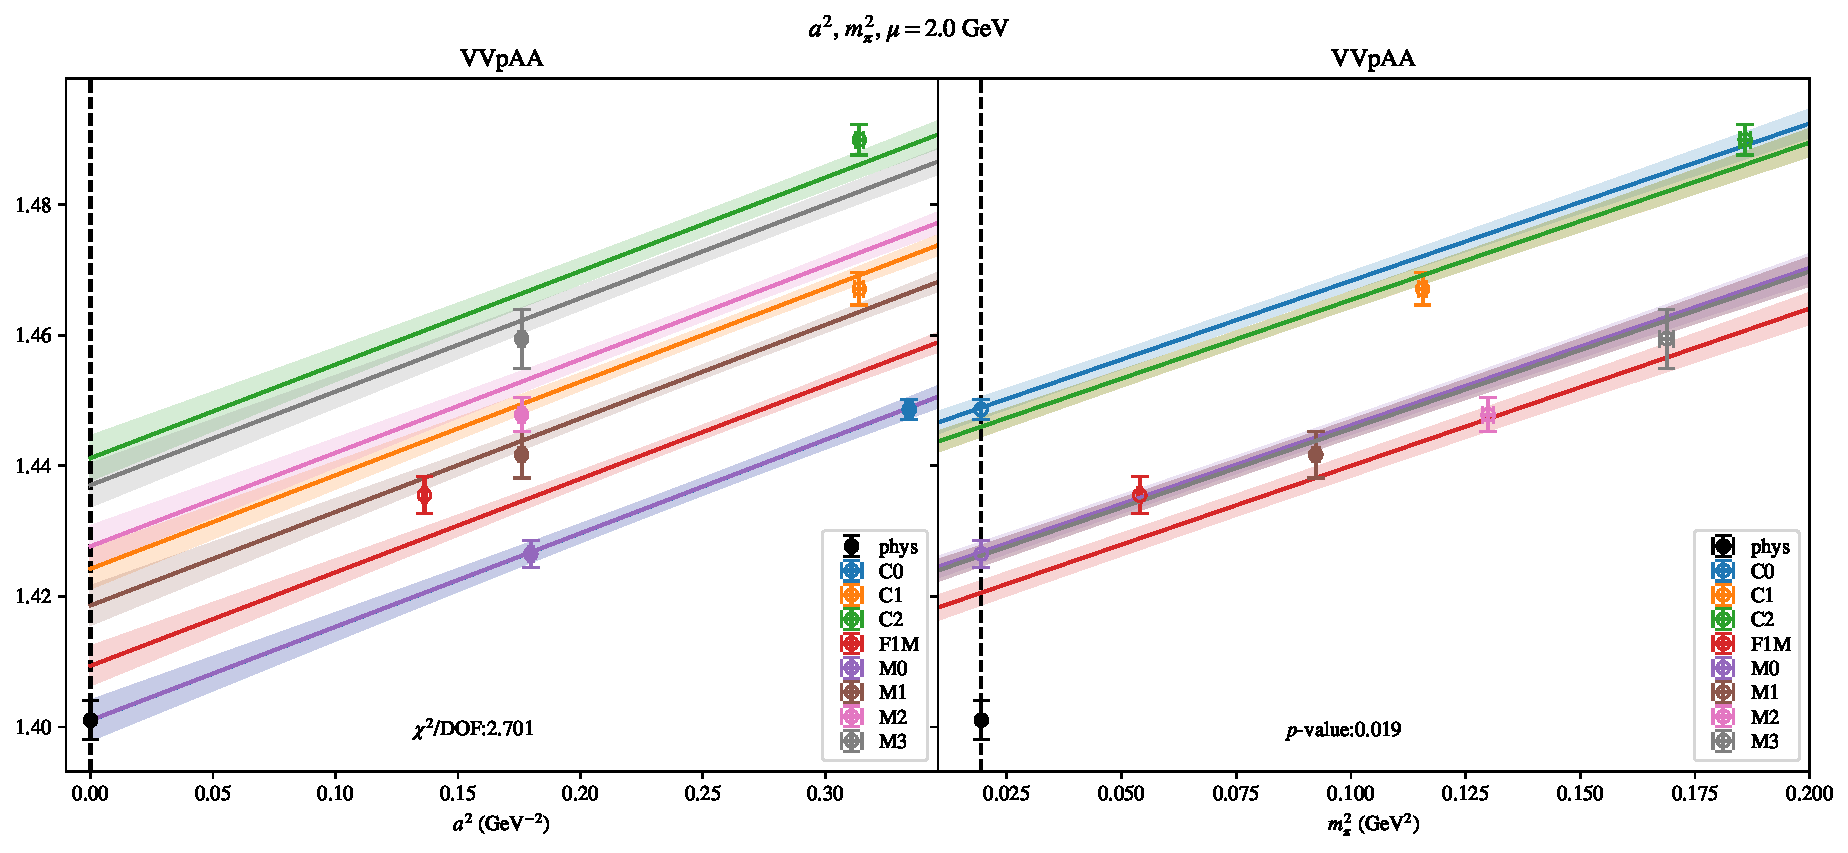
\includepdf[link, pages=-]{VVpAA/SUSY/bag_a2m2_20.pdf}
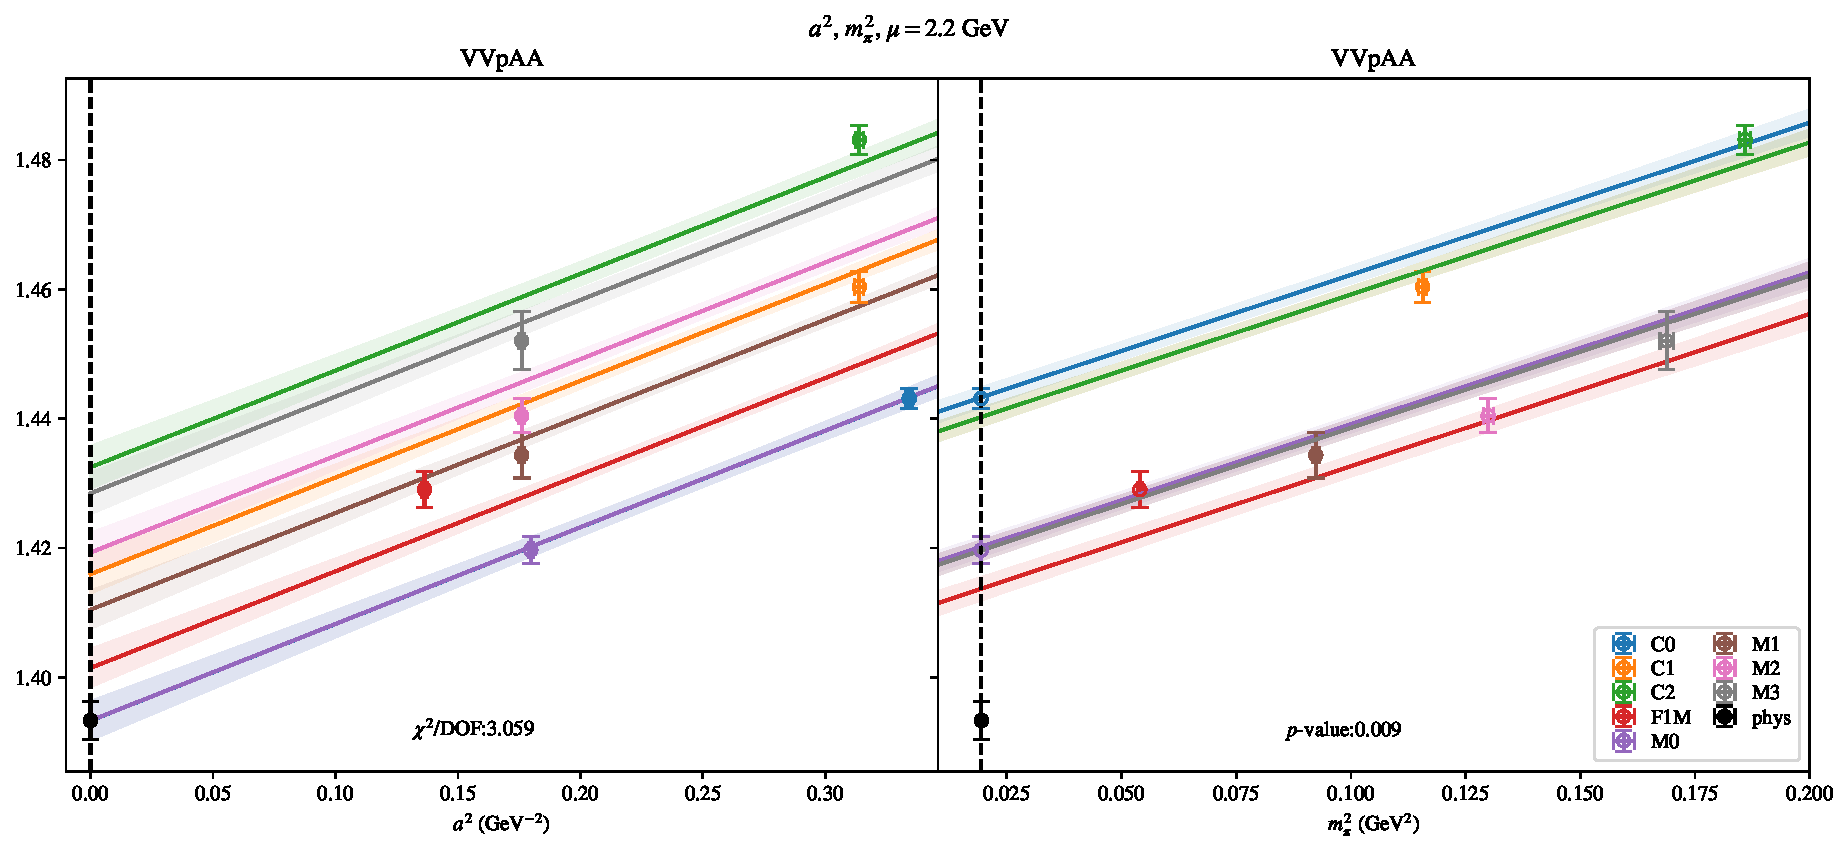
\includepdf[link, pages=-]{VVpAA/SUSY/bag_a2m2_22.pdf}
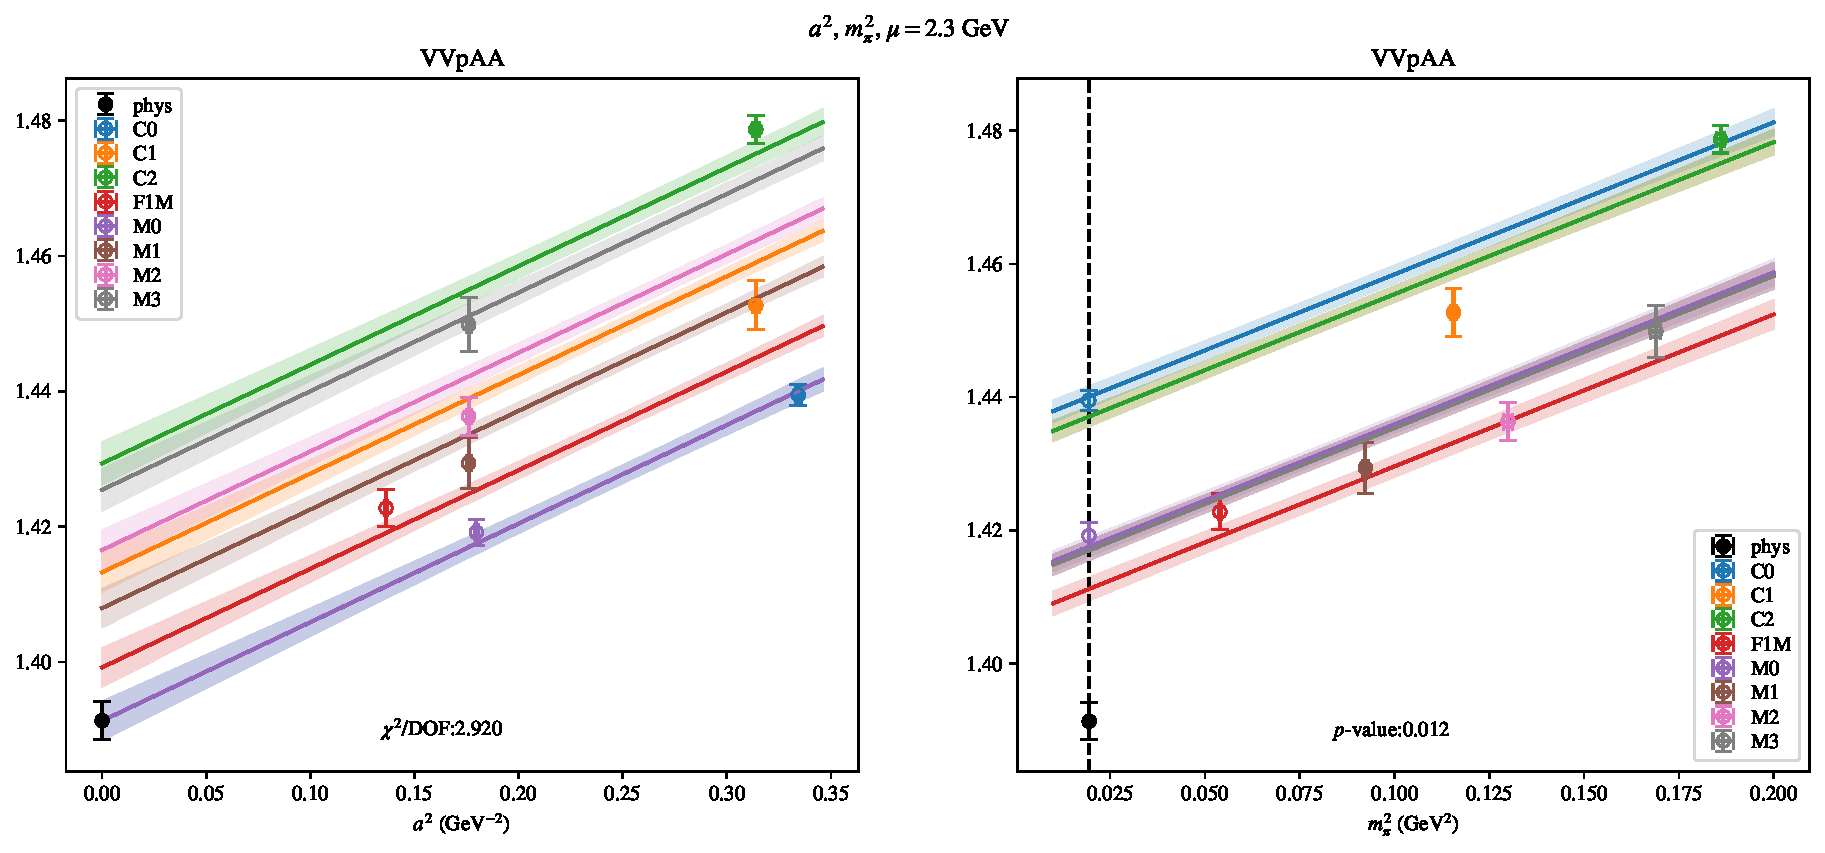
\includepdf[link, pages=-]{VVpAA/SUSY/bag_a2m2_23.pdf}
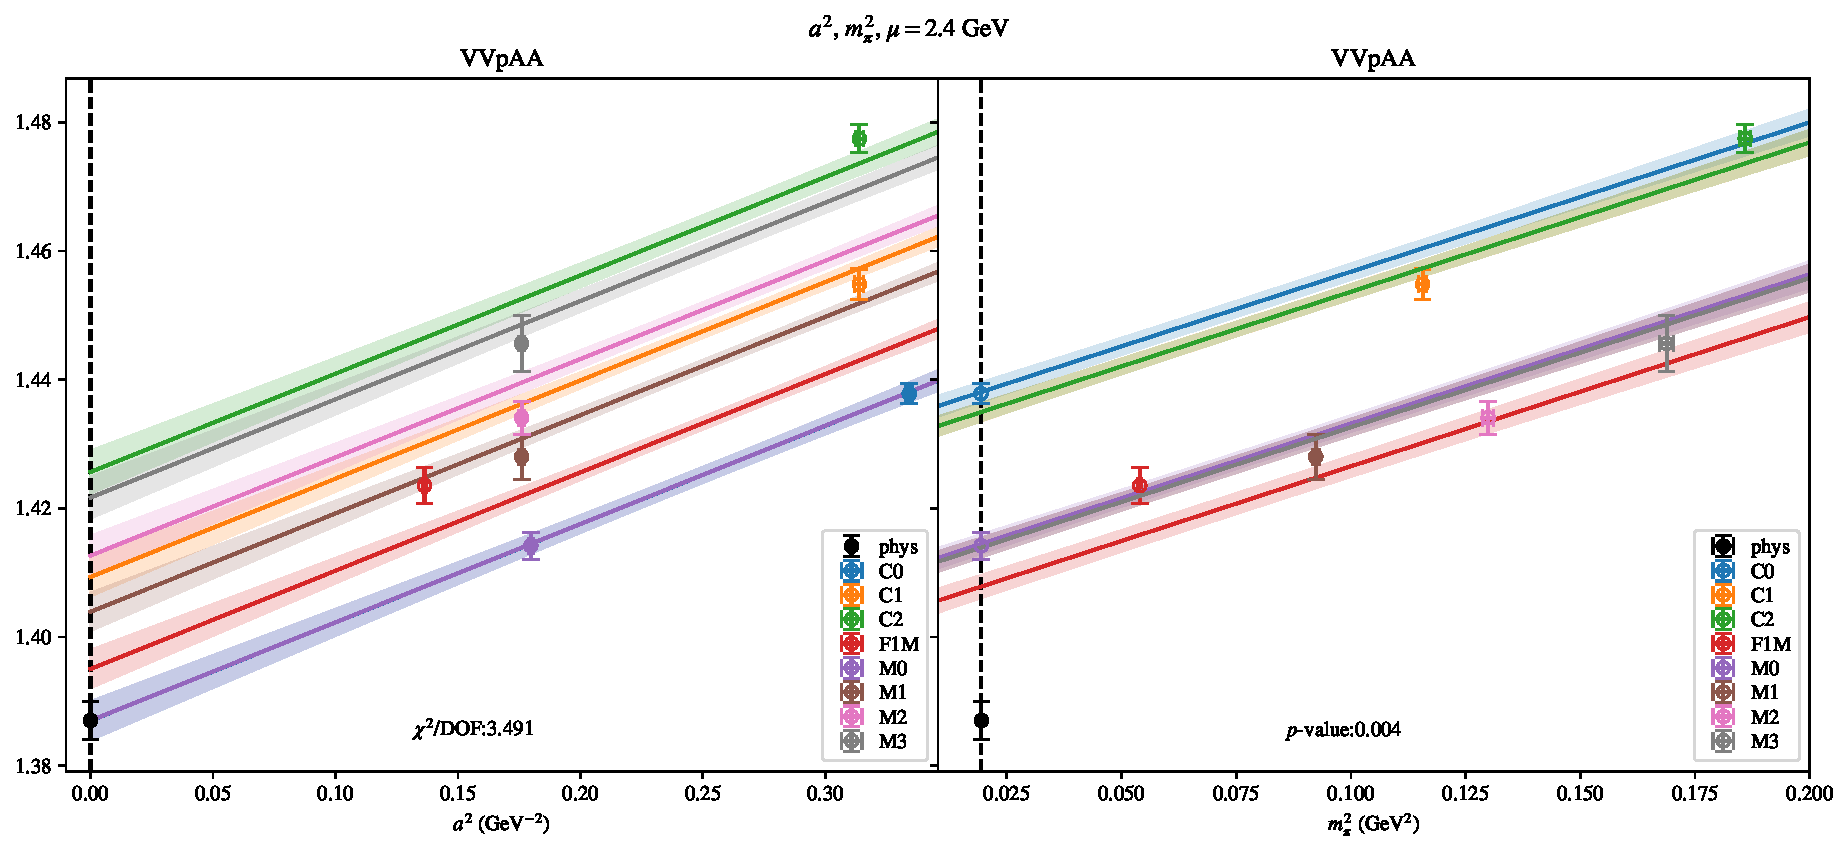
\includepdf[link, pages=-]{VVpAA/SUSY/bag_a2m2_24.pdf}
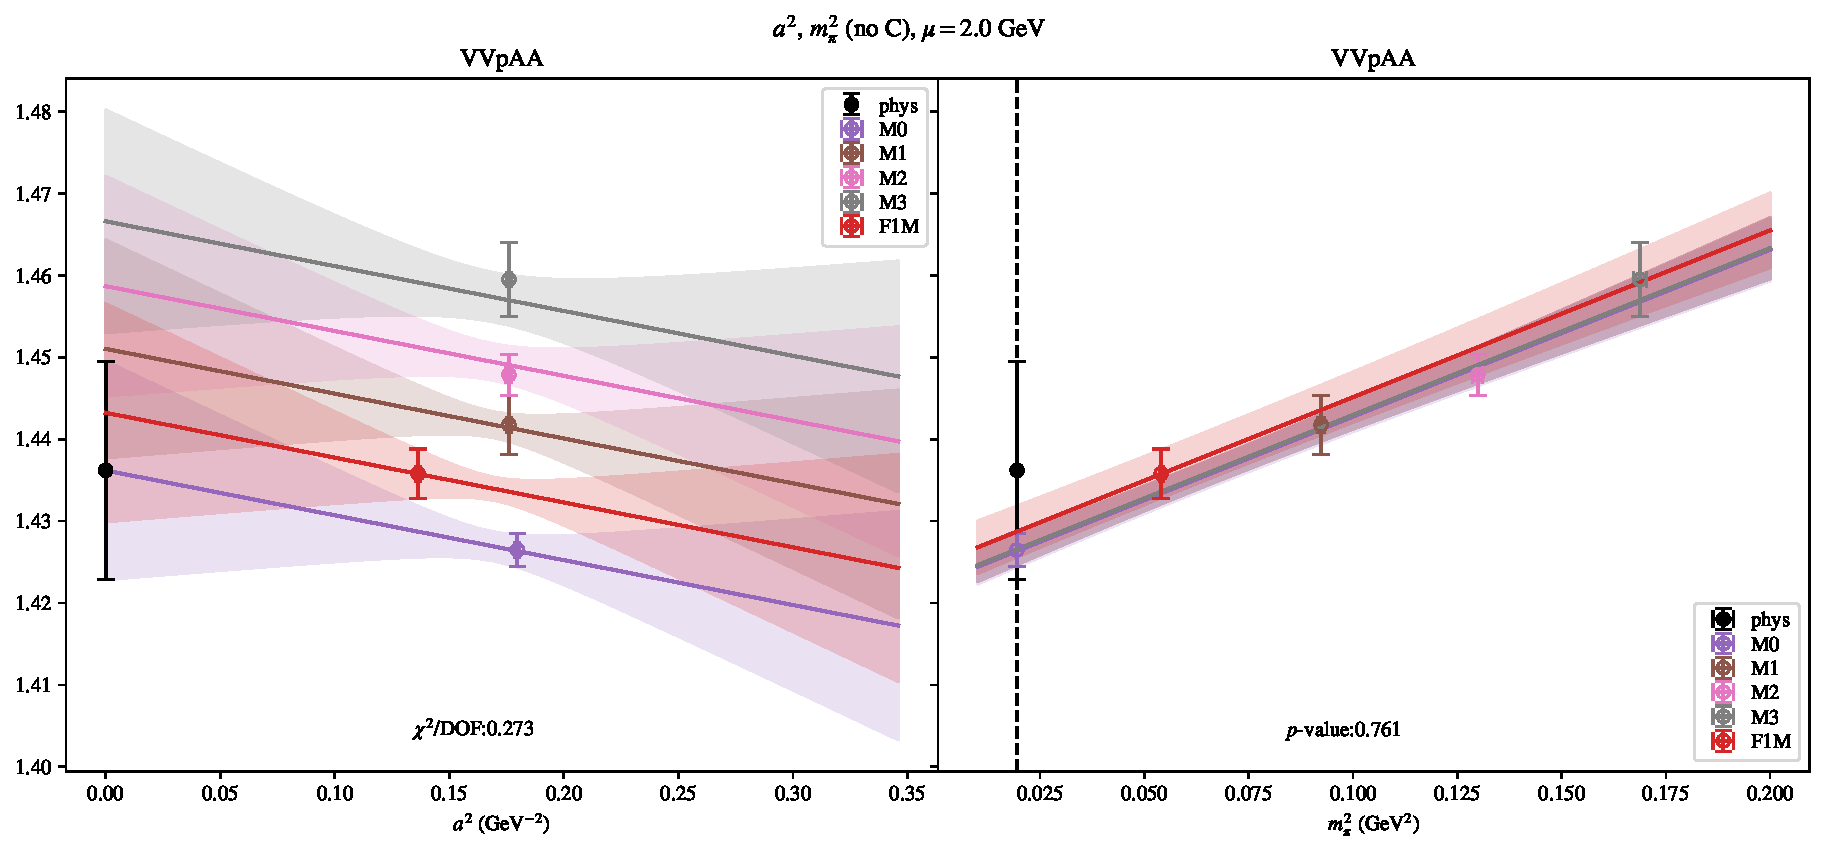
\includepdf[link, pages=-]{VVpAA/SUSY/bag_a2m2noC_20.pdf}
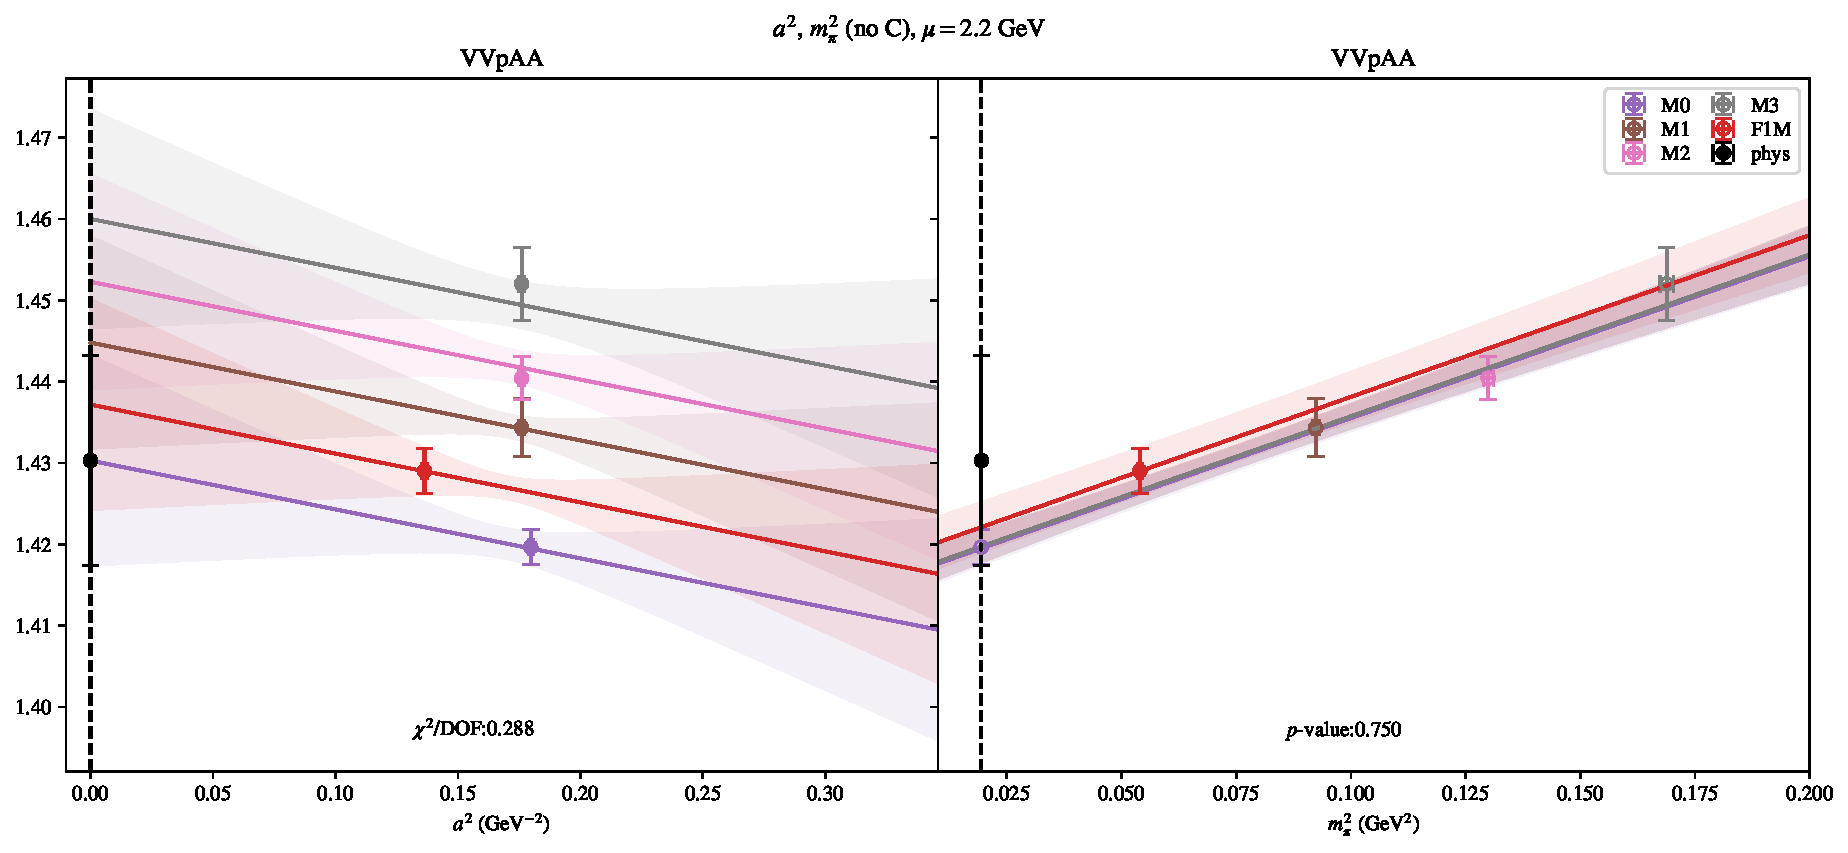
\includepdf[link, pages=-]{VVpAA/SUSY/bag_a2m2noC_22.pdf}
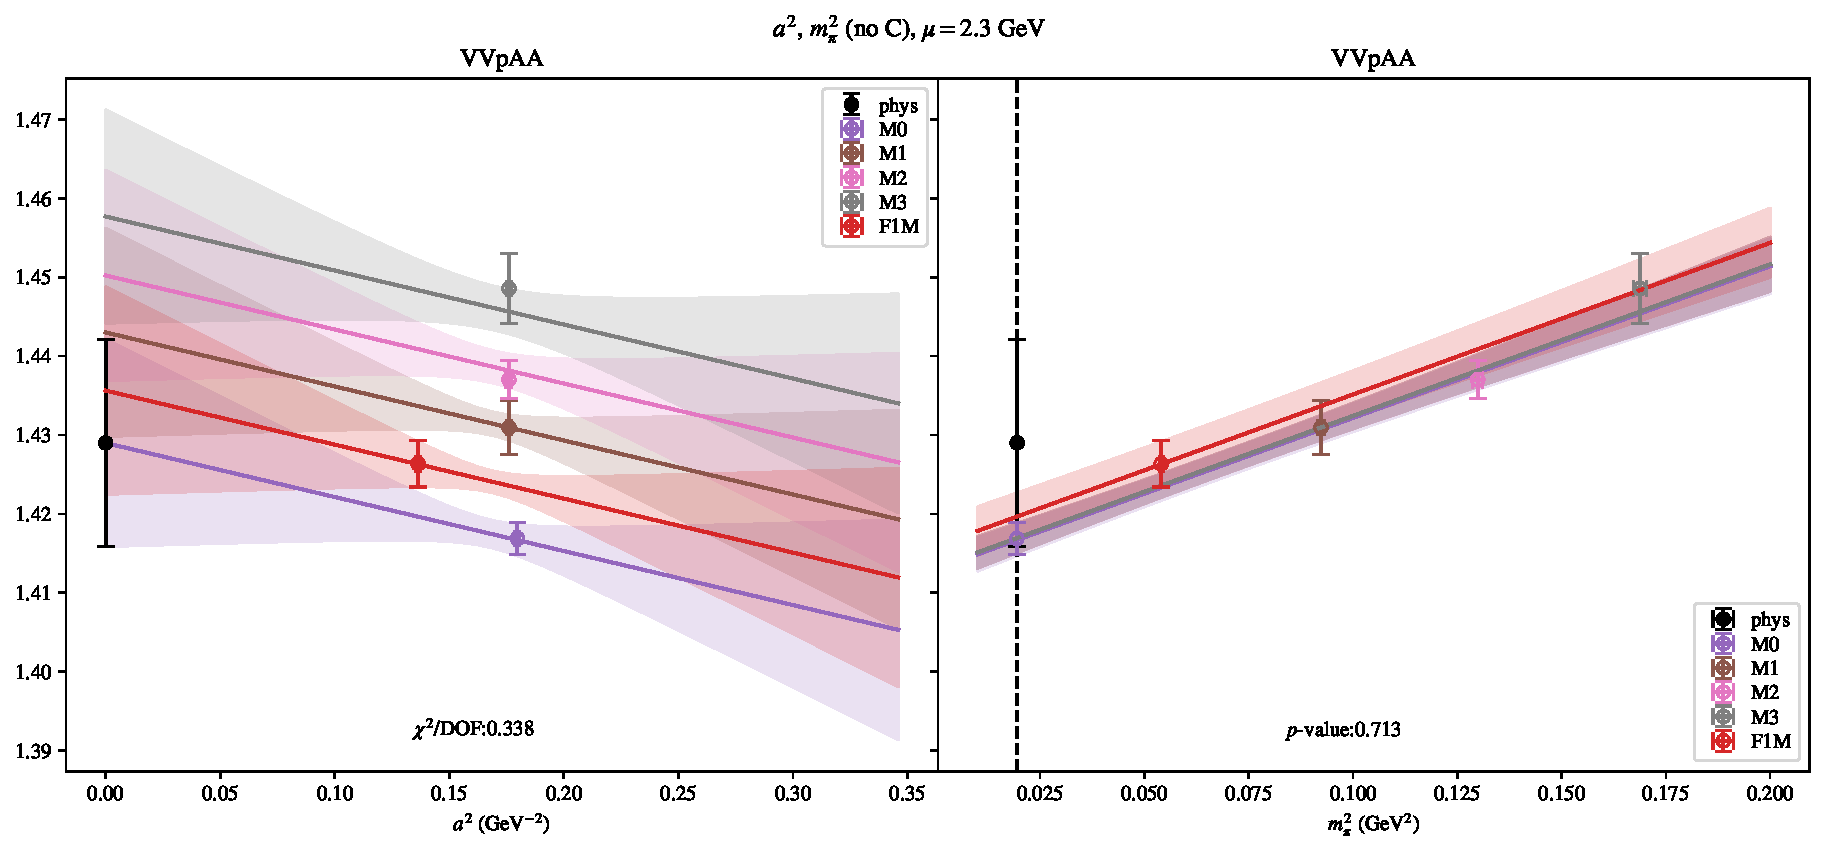
\includepdf[link, pages=-]{VVpAA/SUSY/bag_a2m2noC_23.pdf}
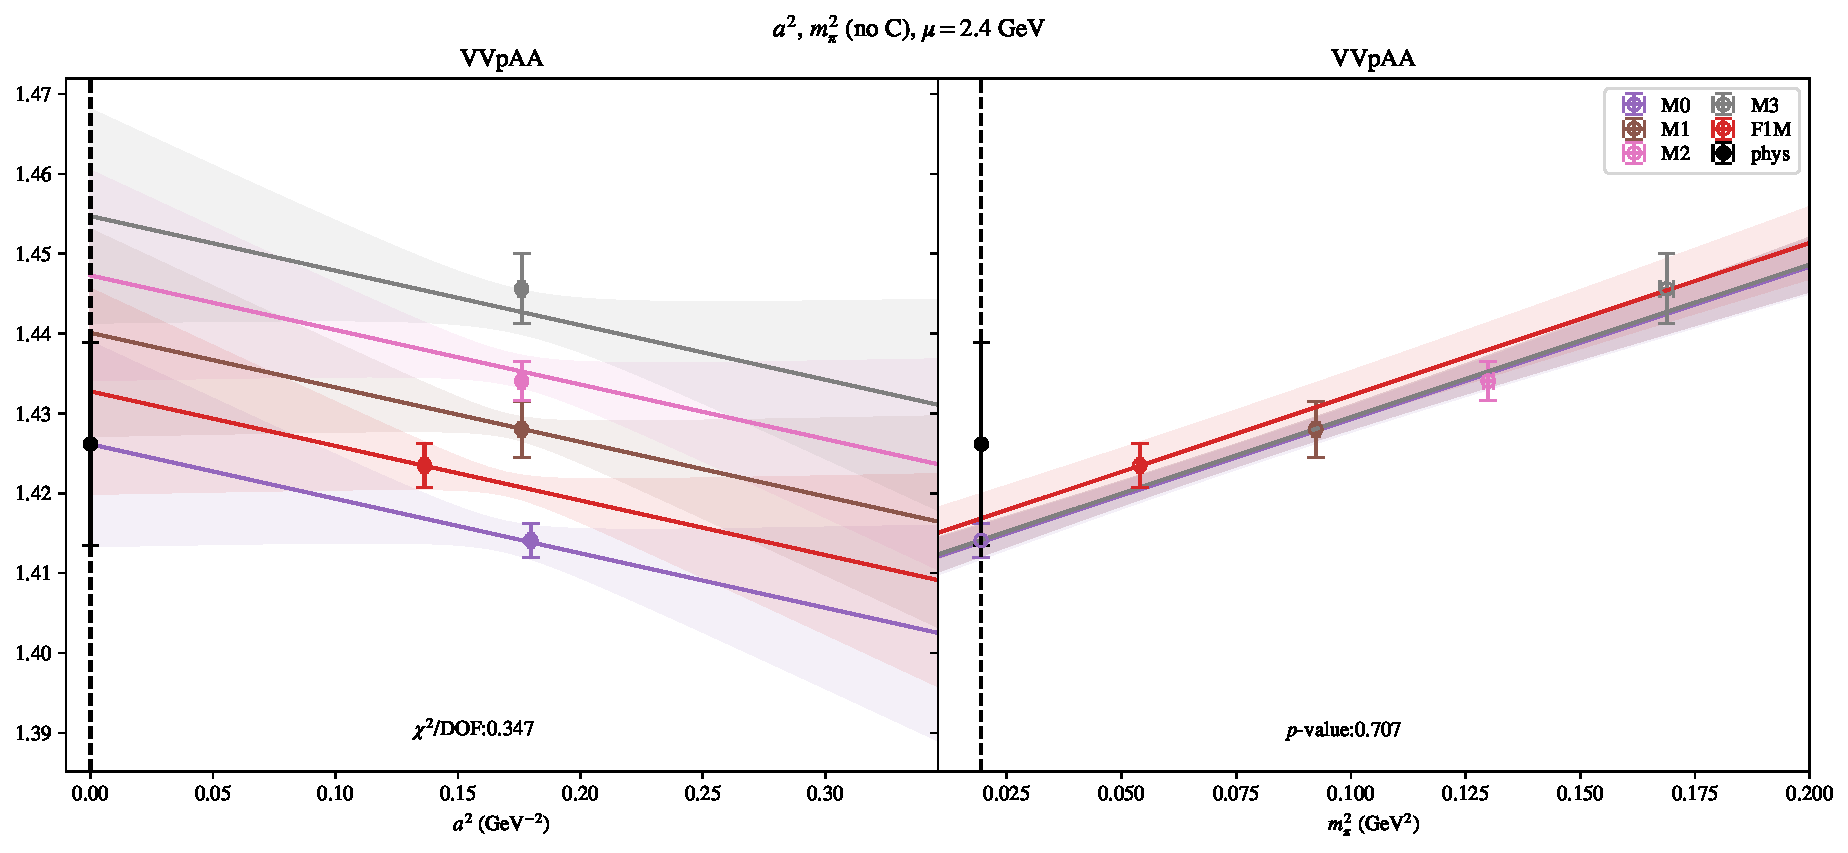
\includepdf[link, pages=-]{VVpAA/SUSY/bag_a2m2noC_24.pdf}
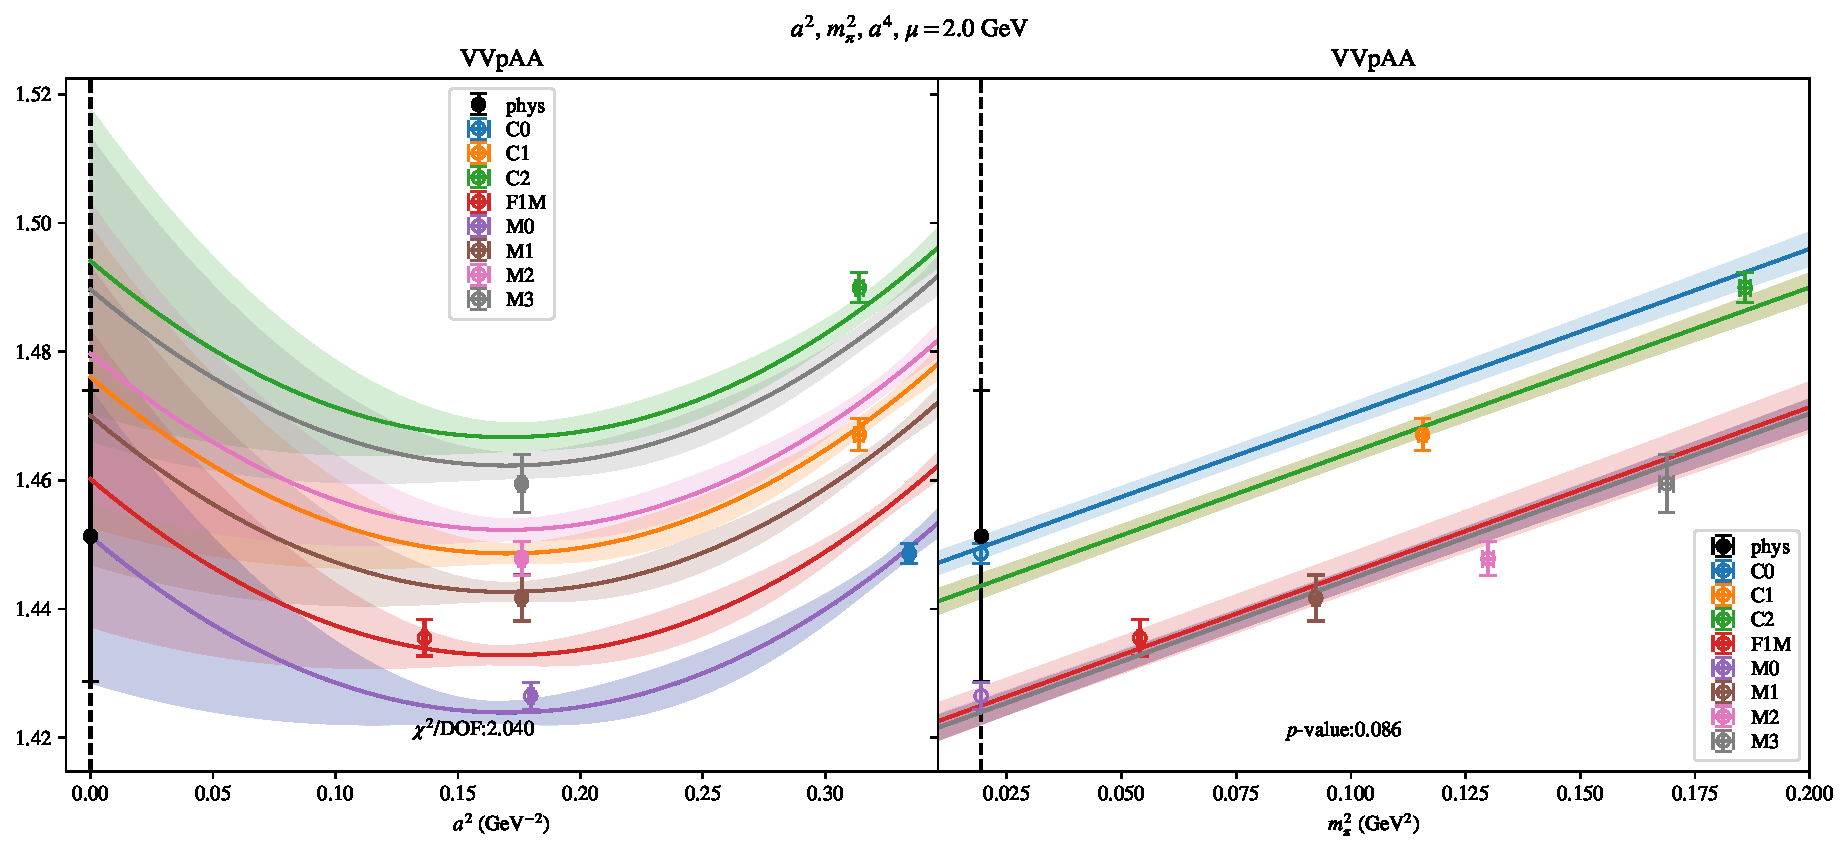
\includepdf[link, pages=-]{VVpAA/SUSY/bag_a2a4m2_20.pdf}
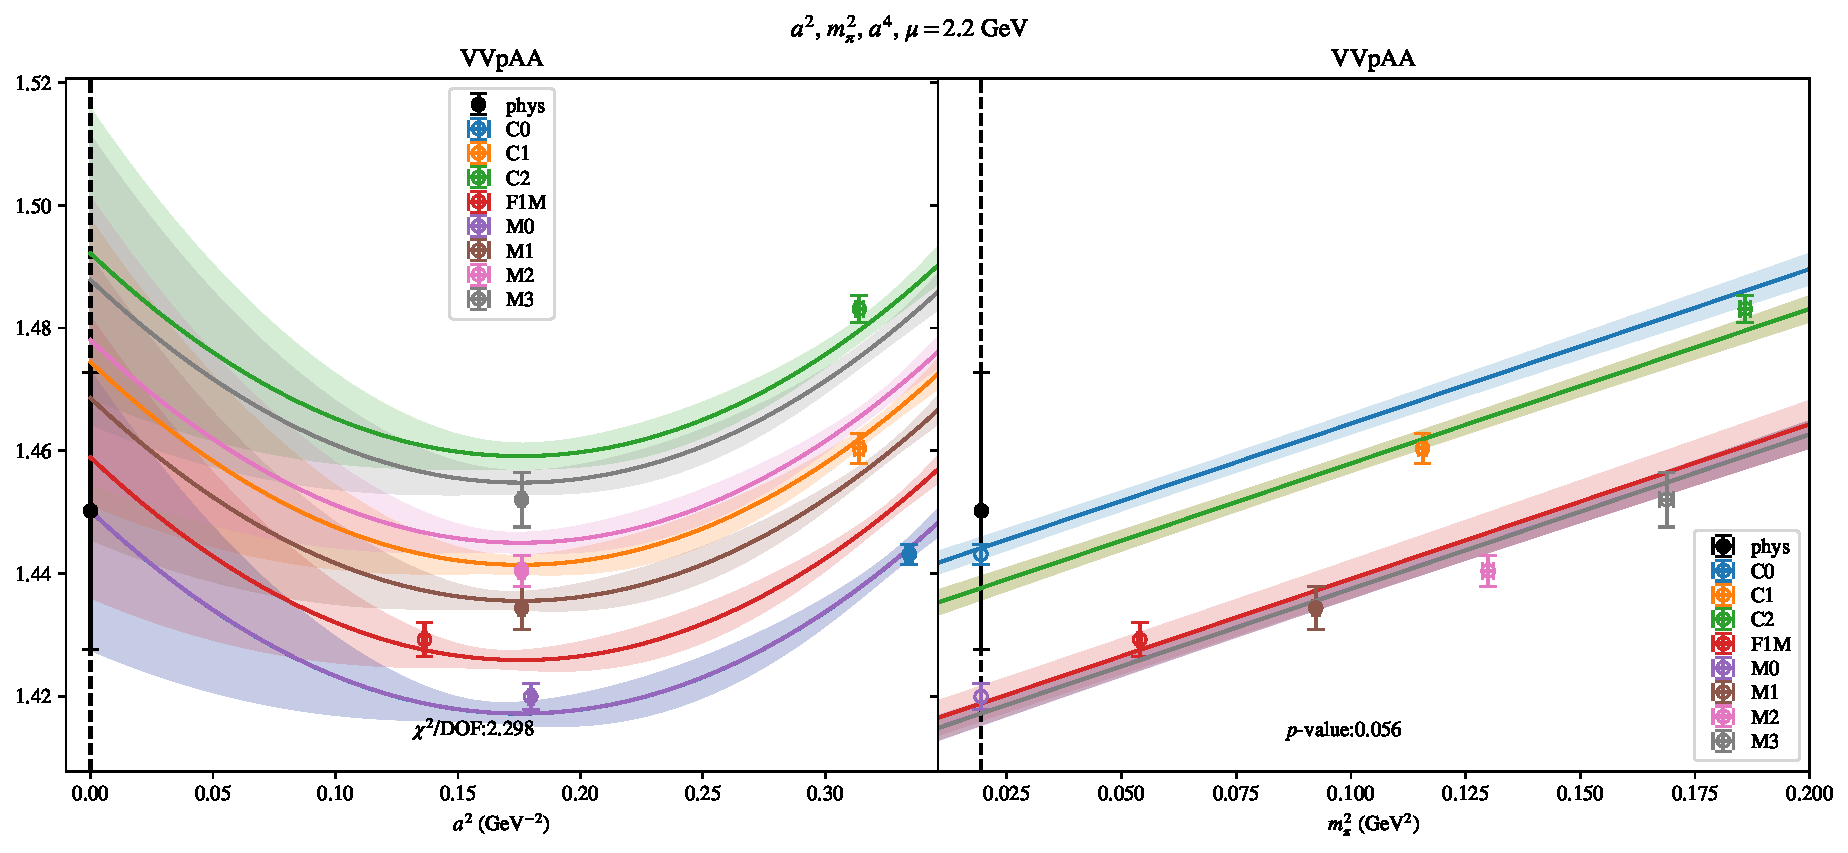
\includepdf[link, pages=-]{VVpAA/SUSY/bag_a2a4m2_22.pdf}
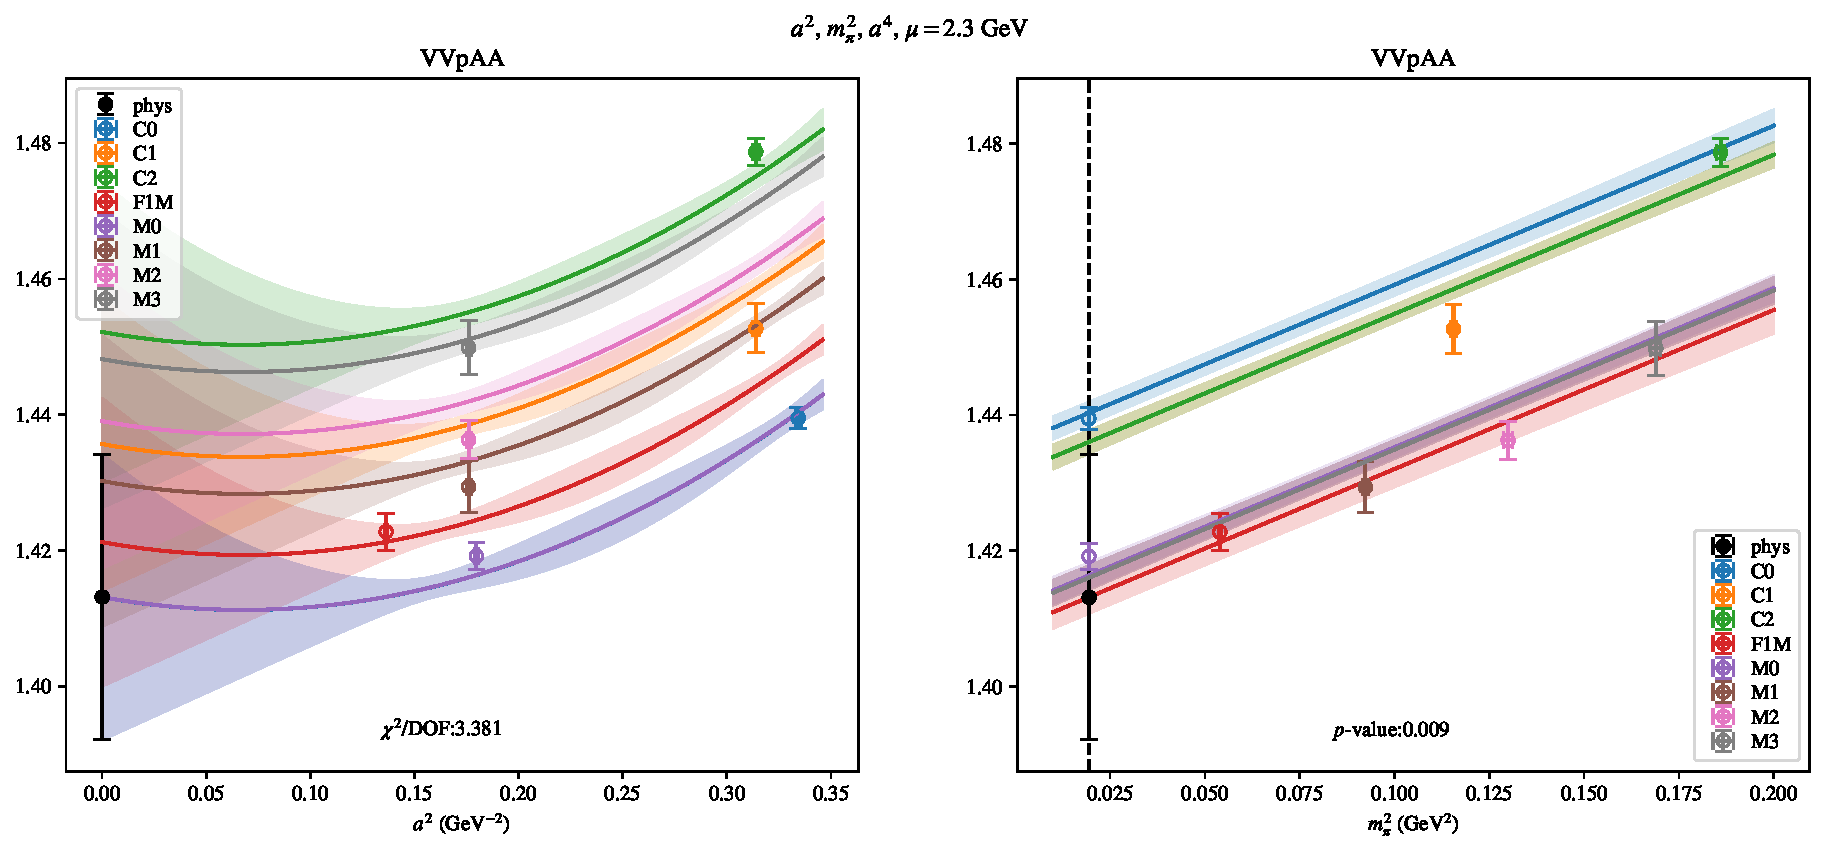
\includepdf[link, pages=-]{VVpAA/SUSY/bag_a2a4m2_23.pdf}
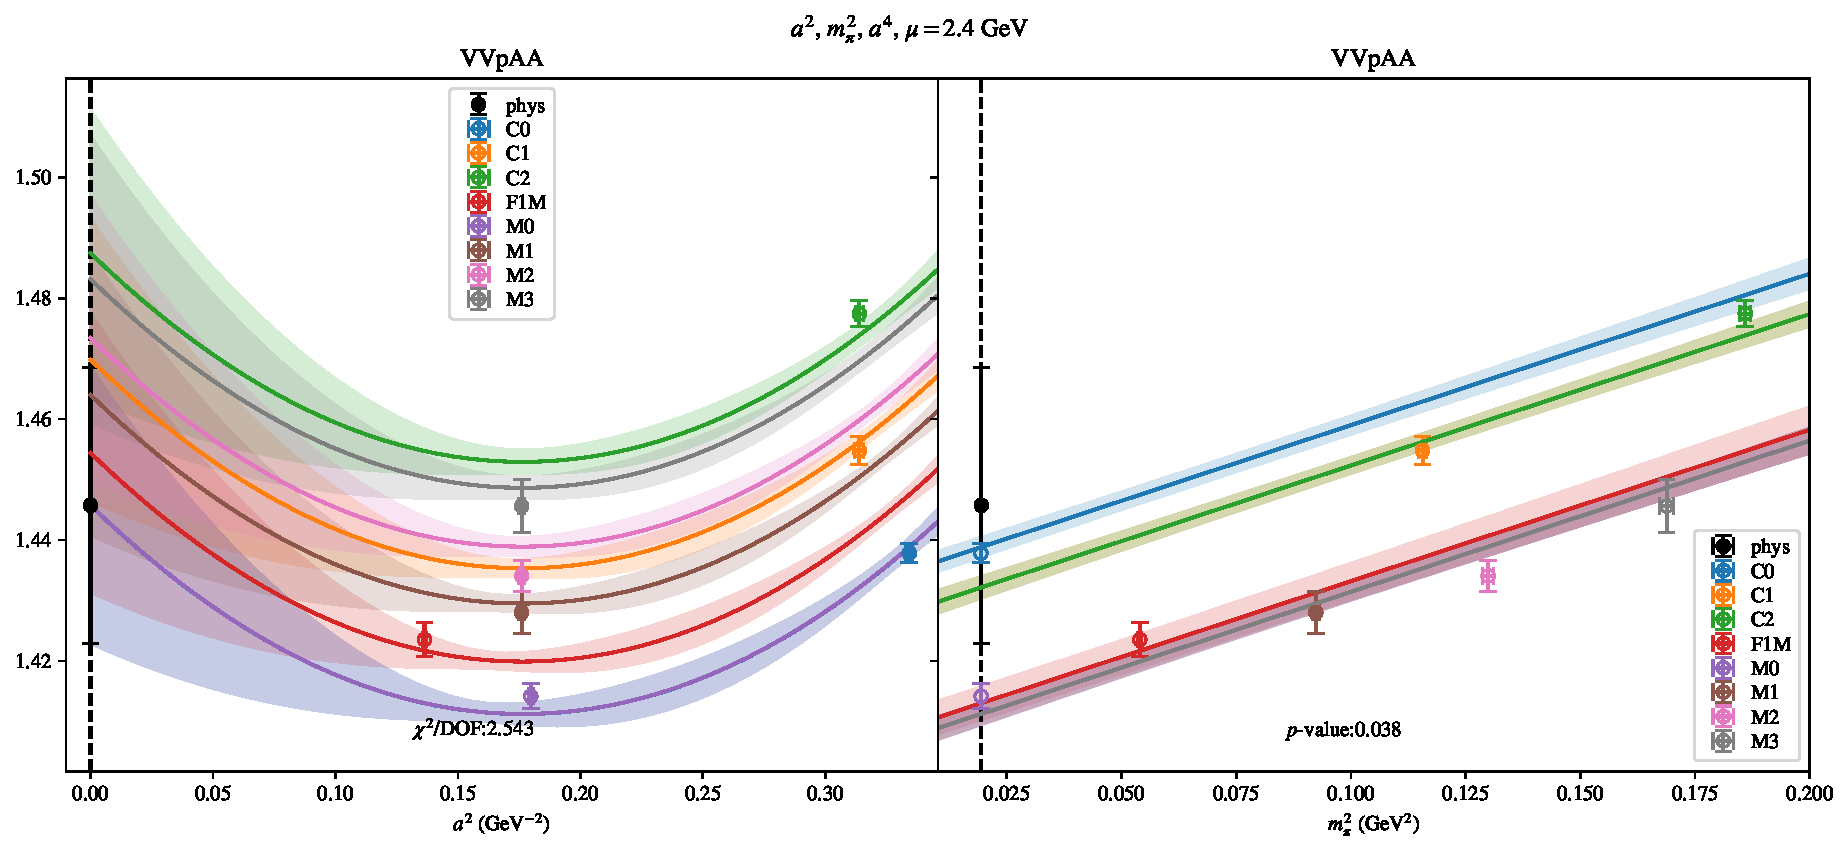
\includepdf[link, pages=-]{VVpAA/SUSY/bag_a2a4m2_24.pdf}
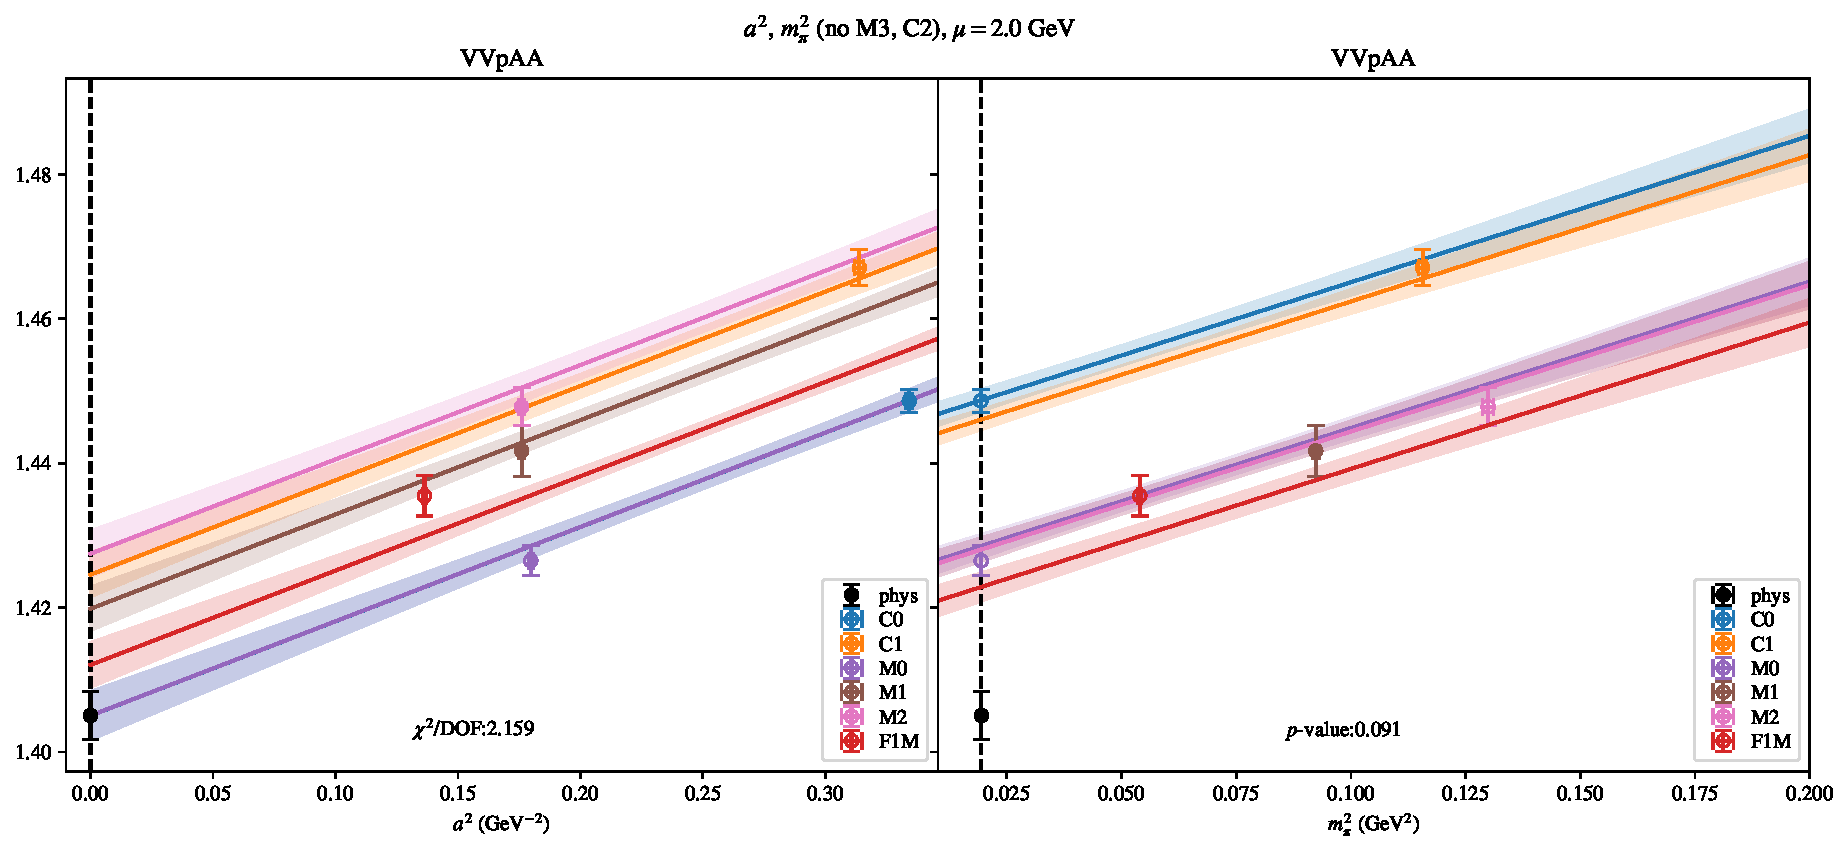
\includepdf[link, pages=-]{VVpAA/SUSY/bag_a2m2mcut_20.pdf}
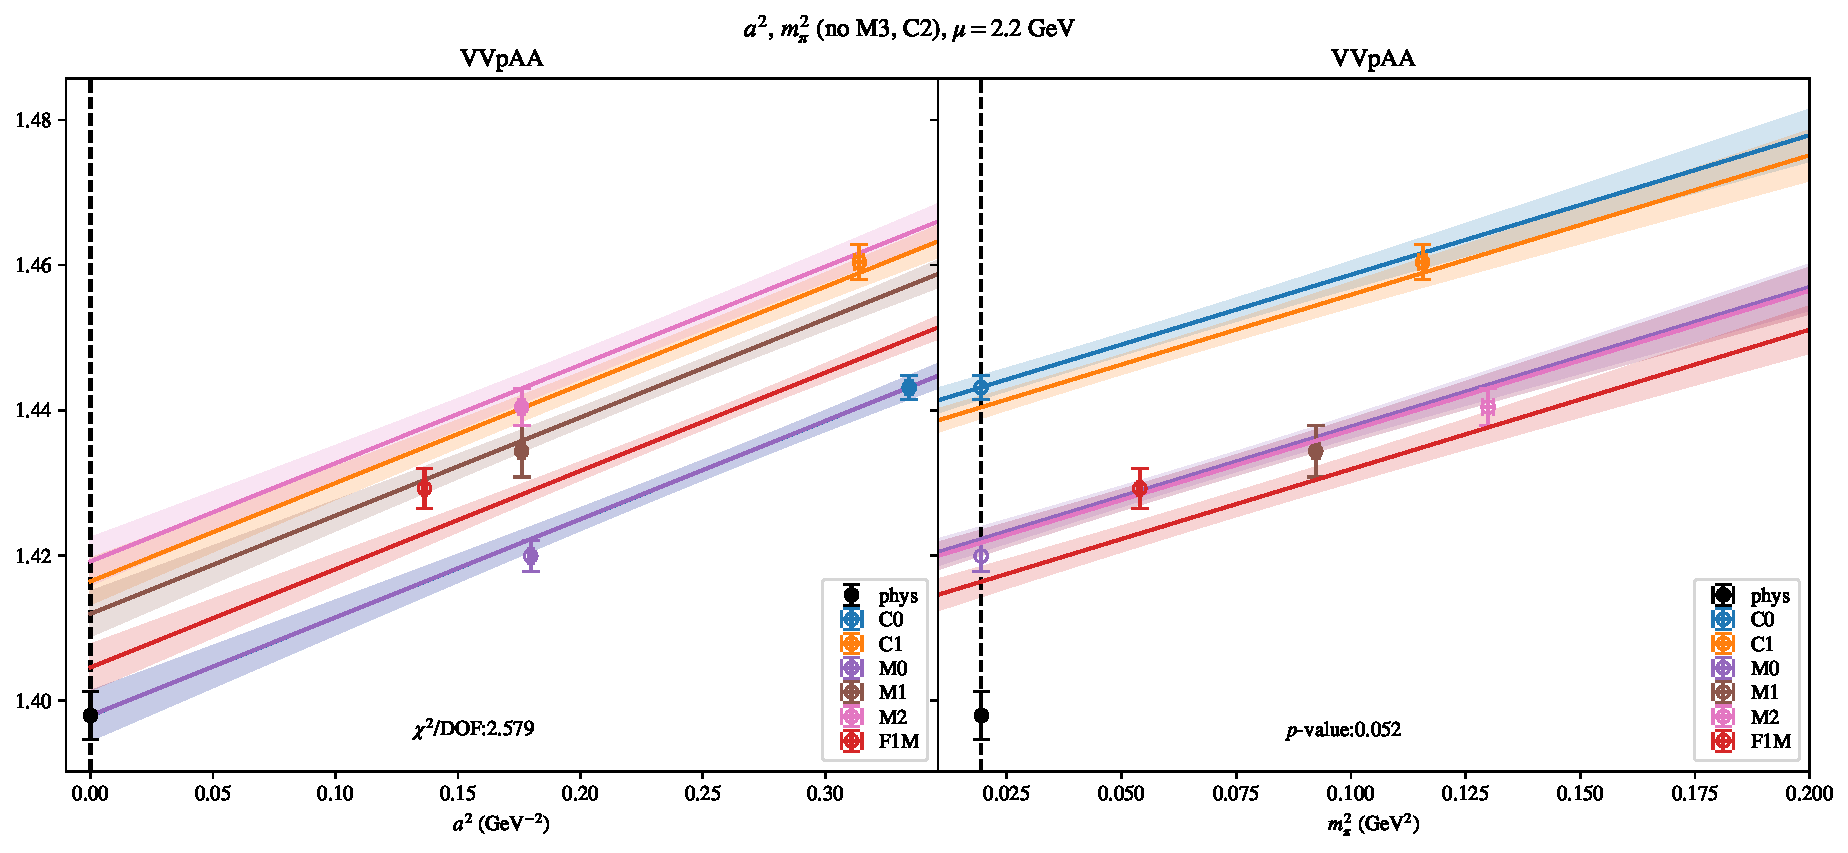
\includepdf[link, pages=-]{VVpAA/SUSY/bag_a2m2mcut_22.pdf}
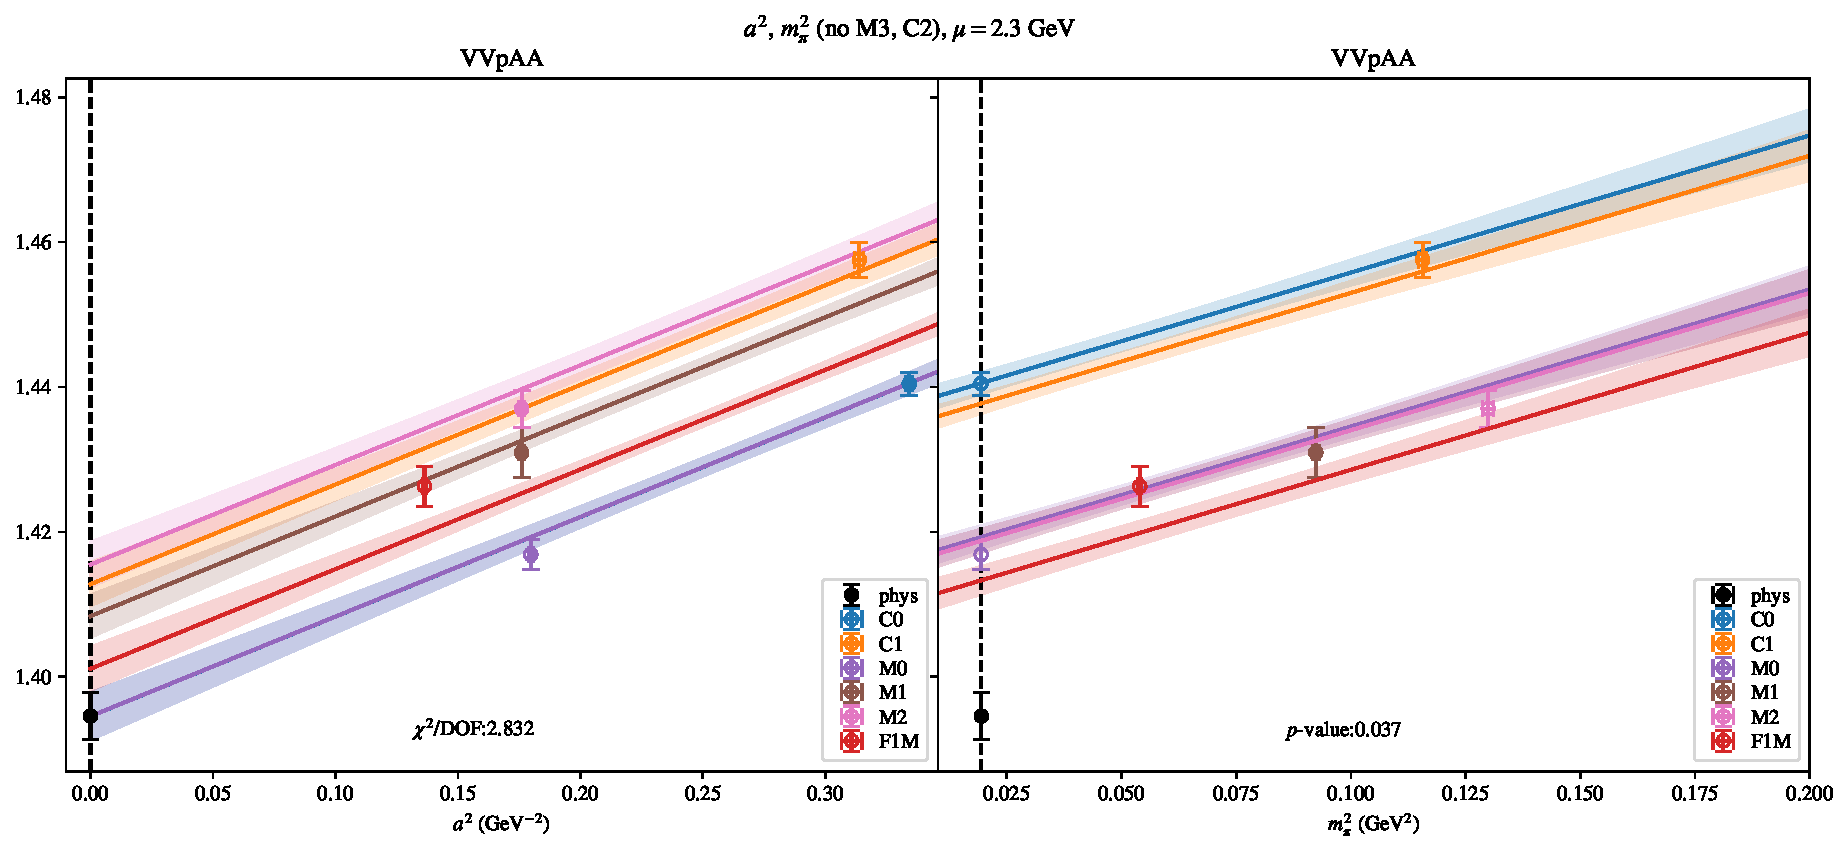
\includepdf[link, pages=-]{VVpAA/SUSY/bag_a2m2mcut_23.pdf}
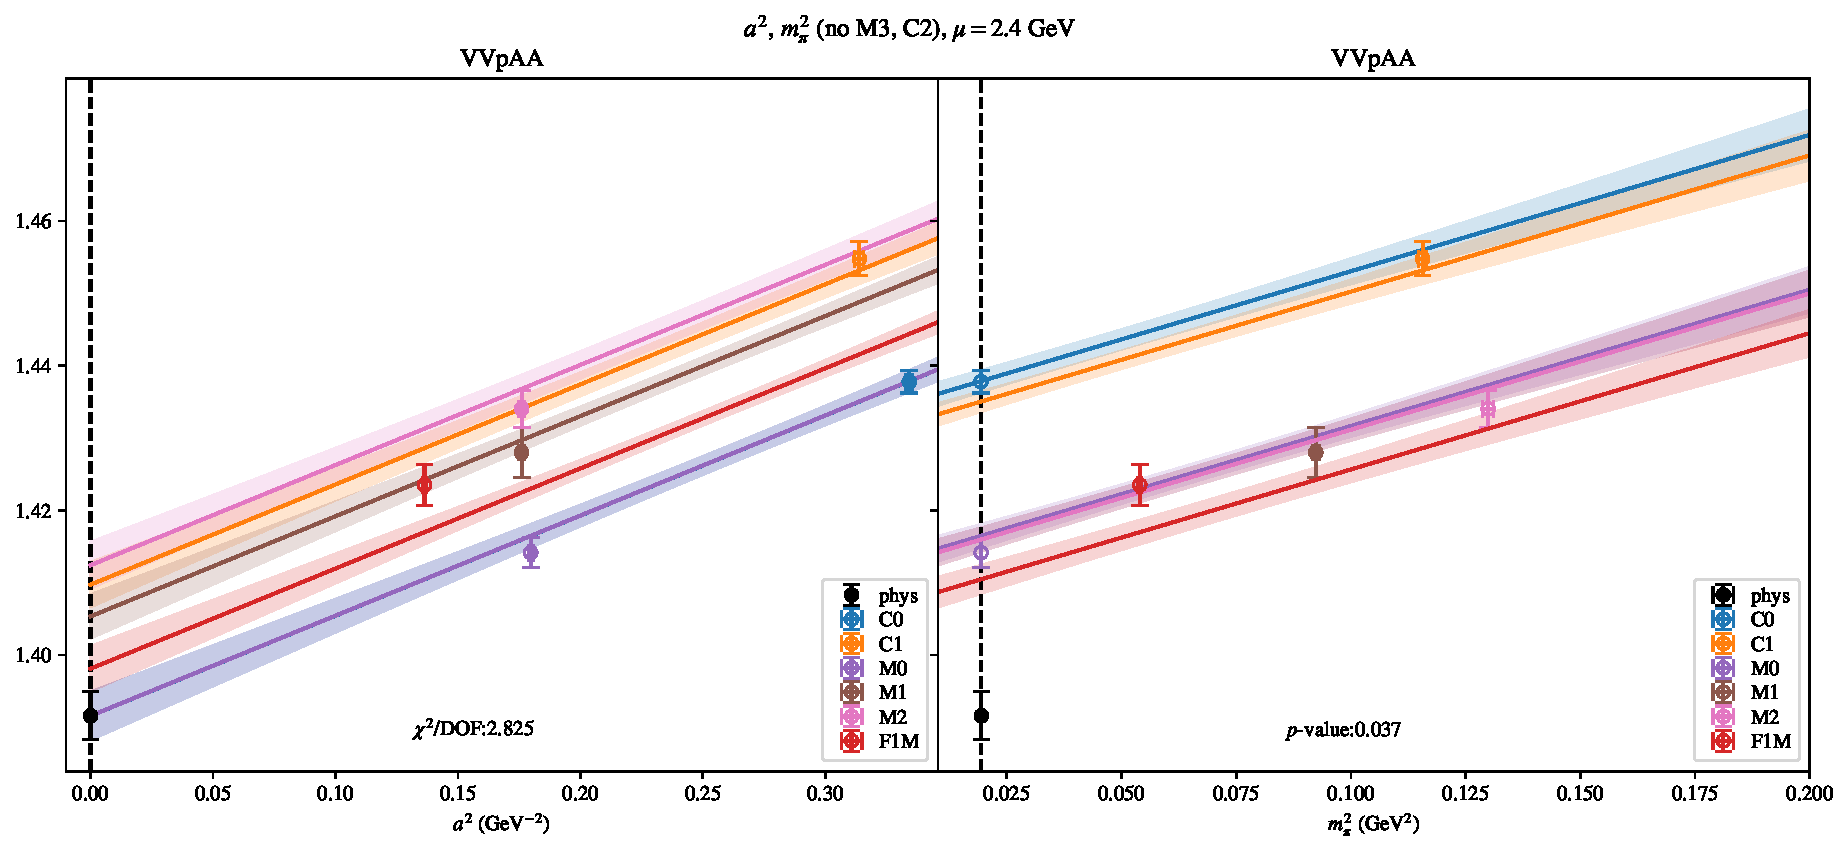
\includepdf[link, pages=-]{VVpAA/SUSY/bag_a2m2mcut_24.pdf}
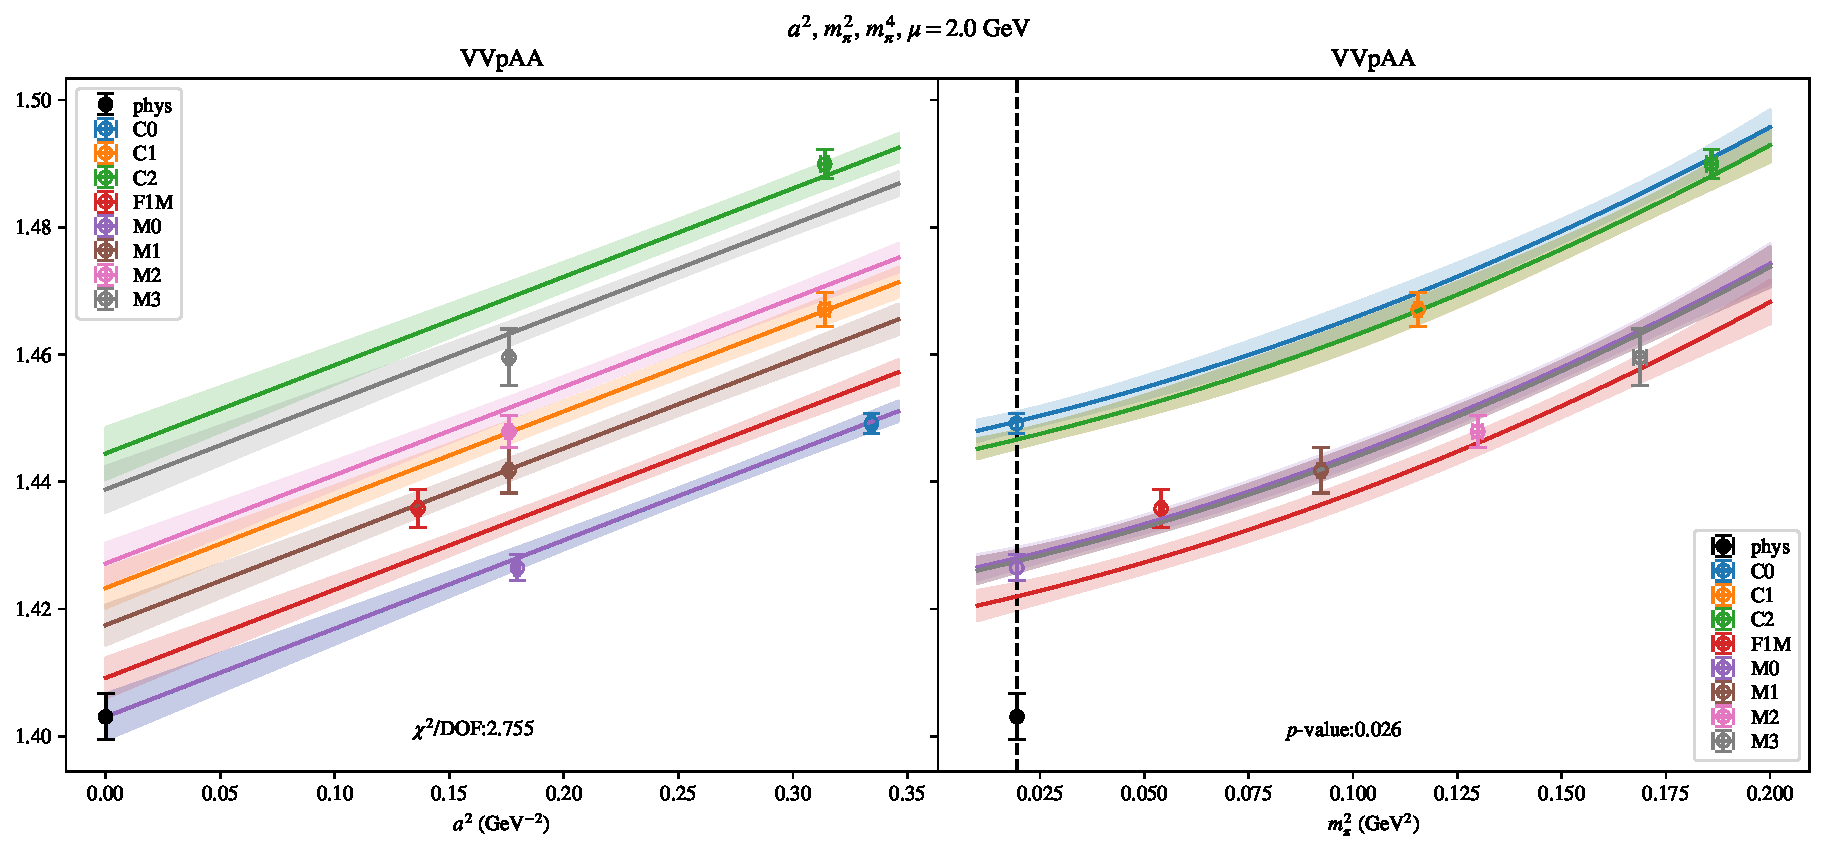
\includepdf[link, pages=-]{VVpAA/SUSY/bag_a2m2m4_20.pdf}
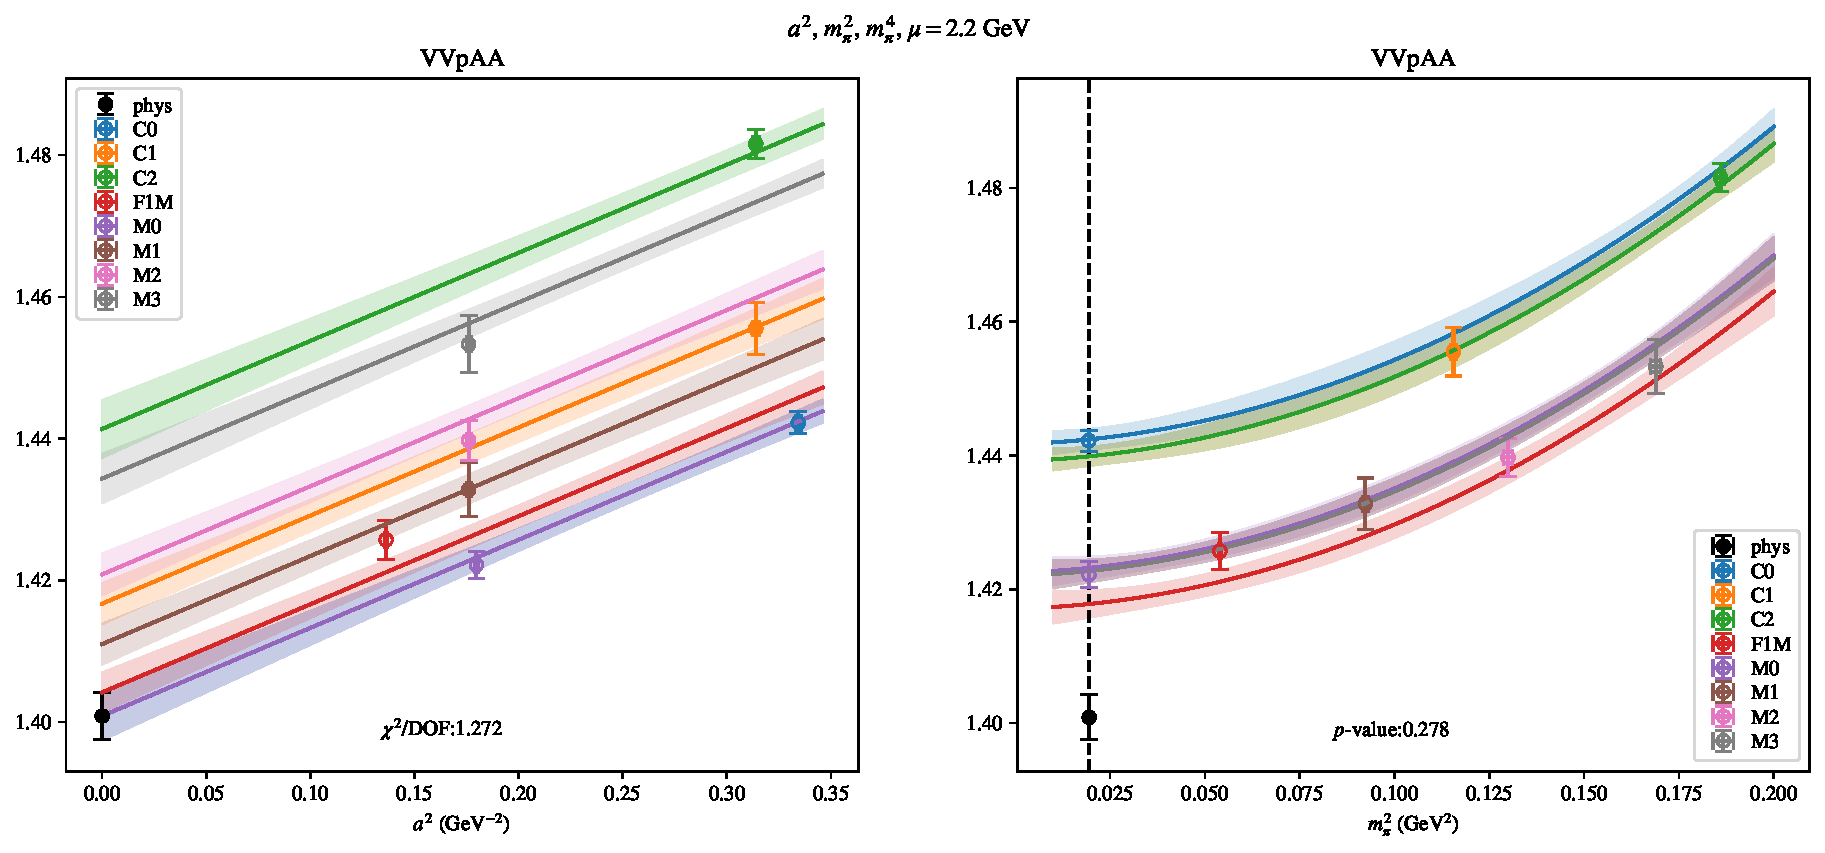
\includepdf[link, pages=-]{VVpAA/SUSY/bag_a2m2m4_22.pdf}
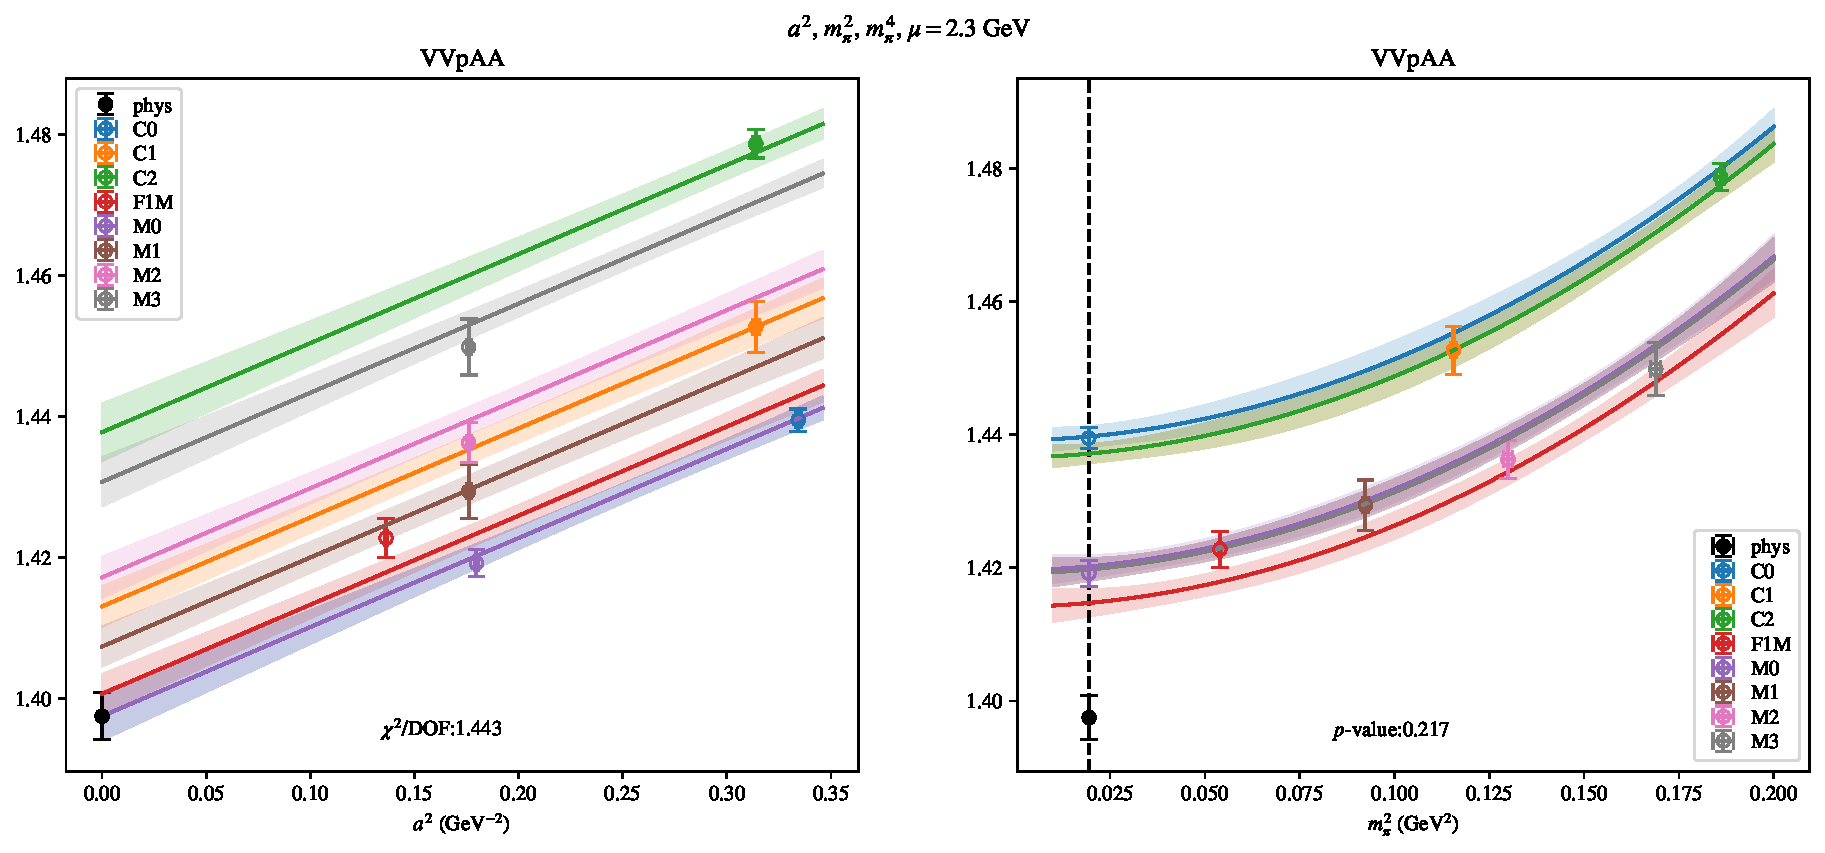
\includepdf[link, pages=-]{VVpAA/SUSY/bag_a2m2m4_23.pdf}
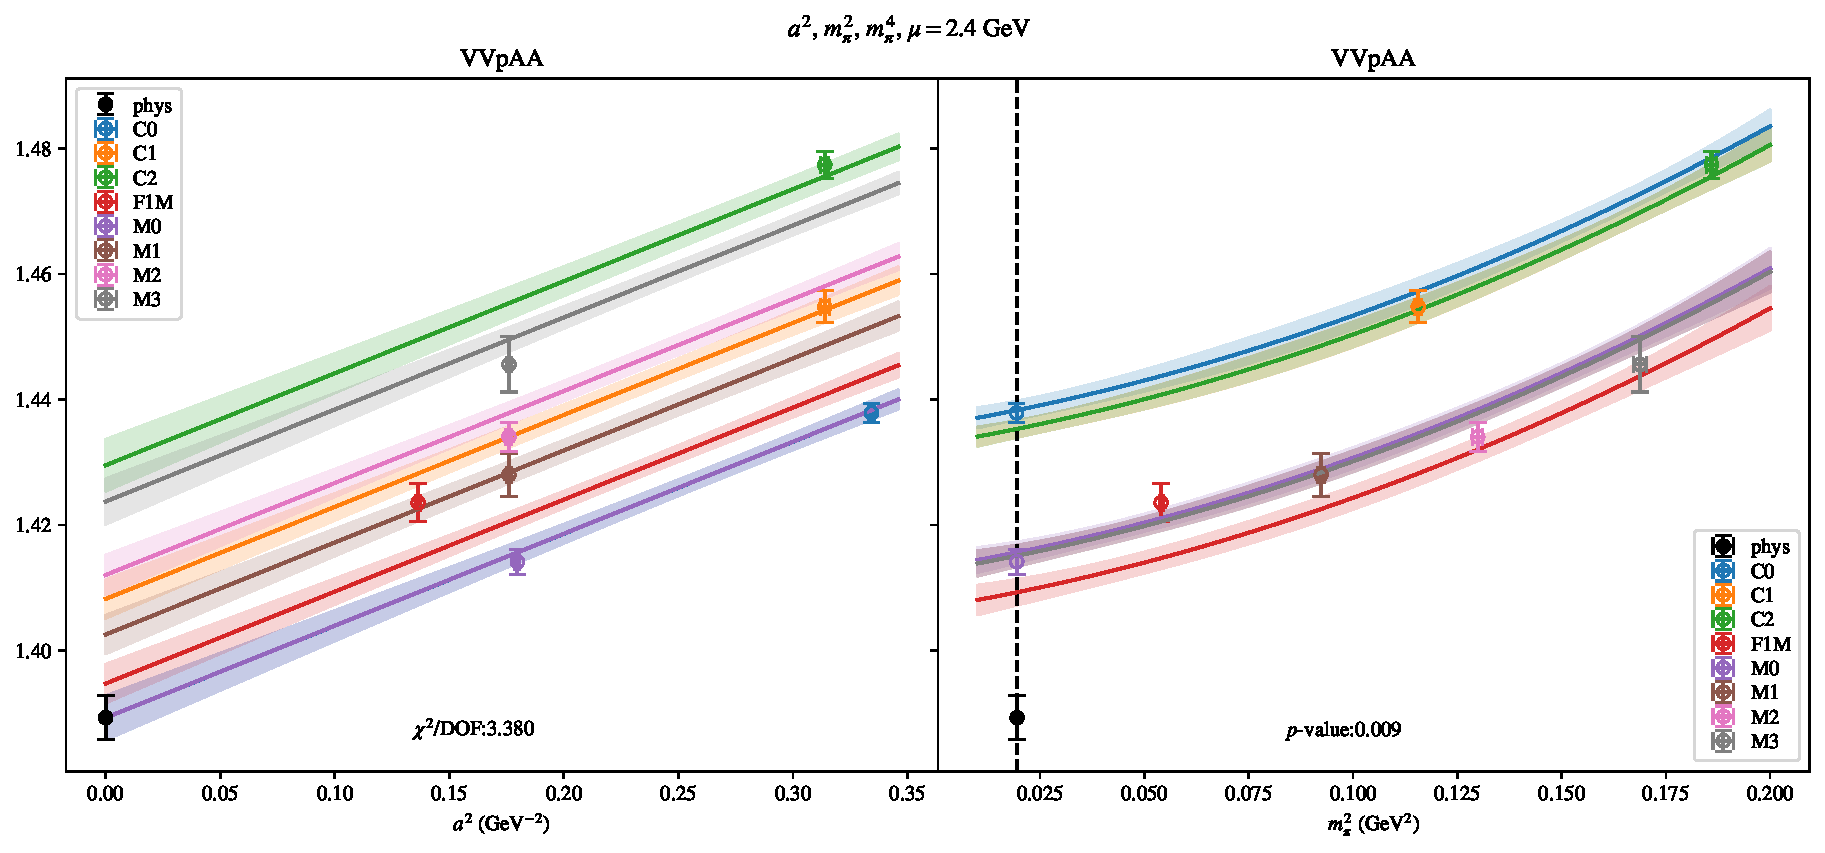
\includepdf[link, pages=-]{VVpAA/SUSY/bag_a2m2m4_24.pdf}
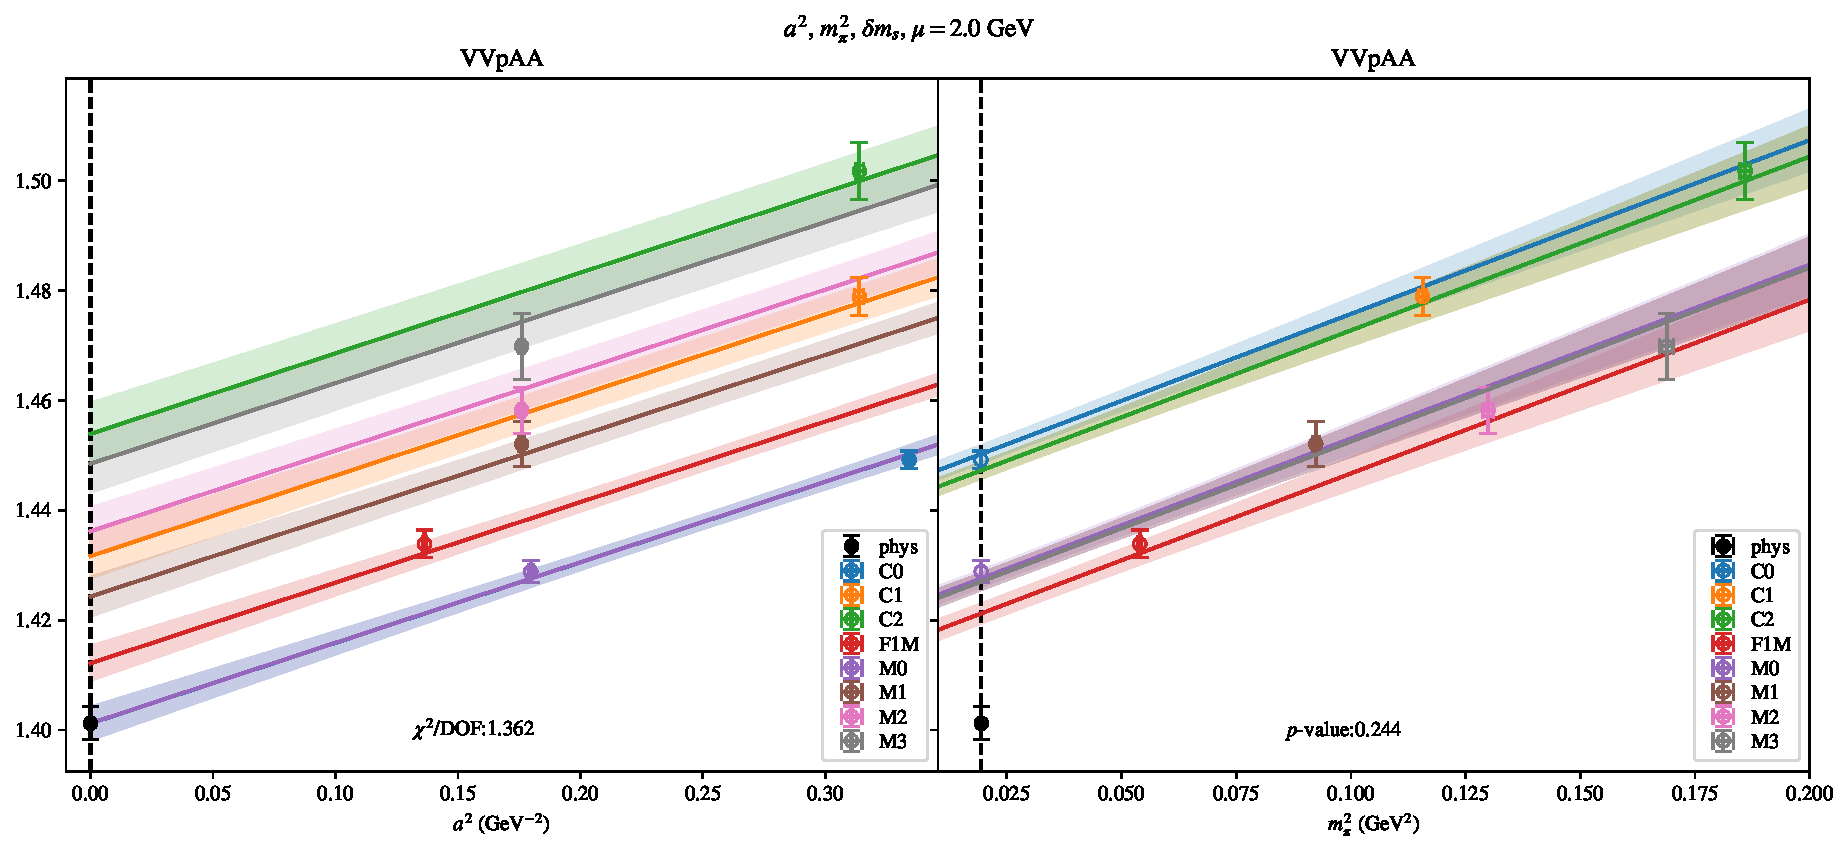
\includepdf[link, pages=-]{VVpAA/SUSY/bag_a2m2delm_20.pdf}
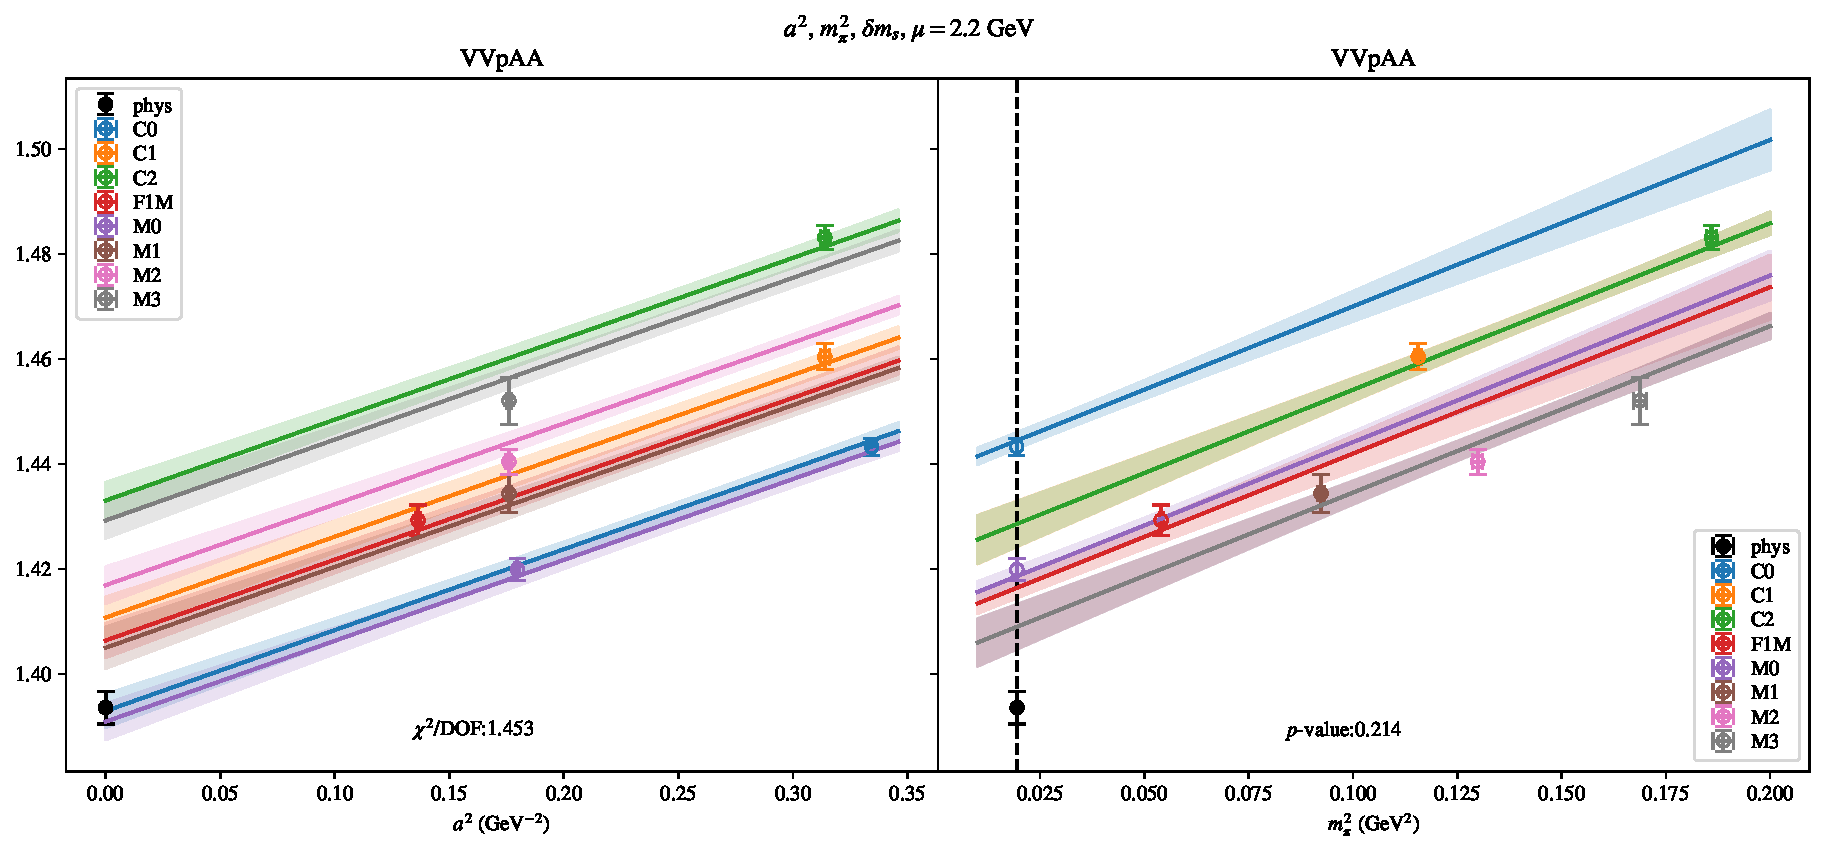
\includepdf[link, pages=-]{VVpAA/SUSY/bag_a2m2delm_22.pdf}
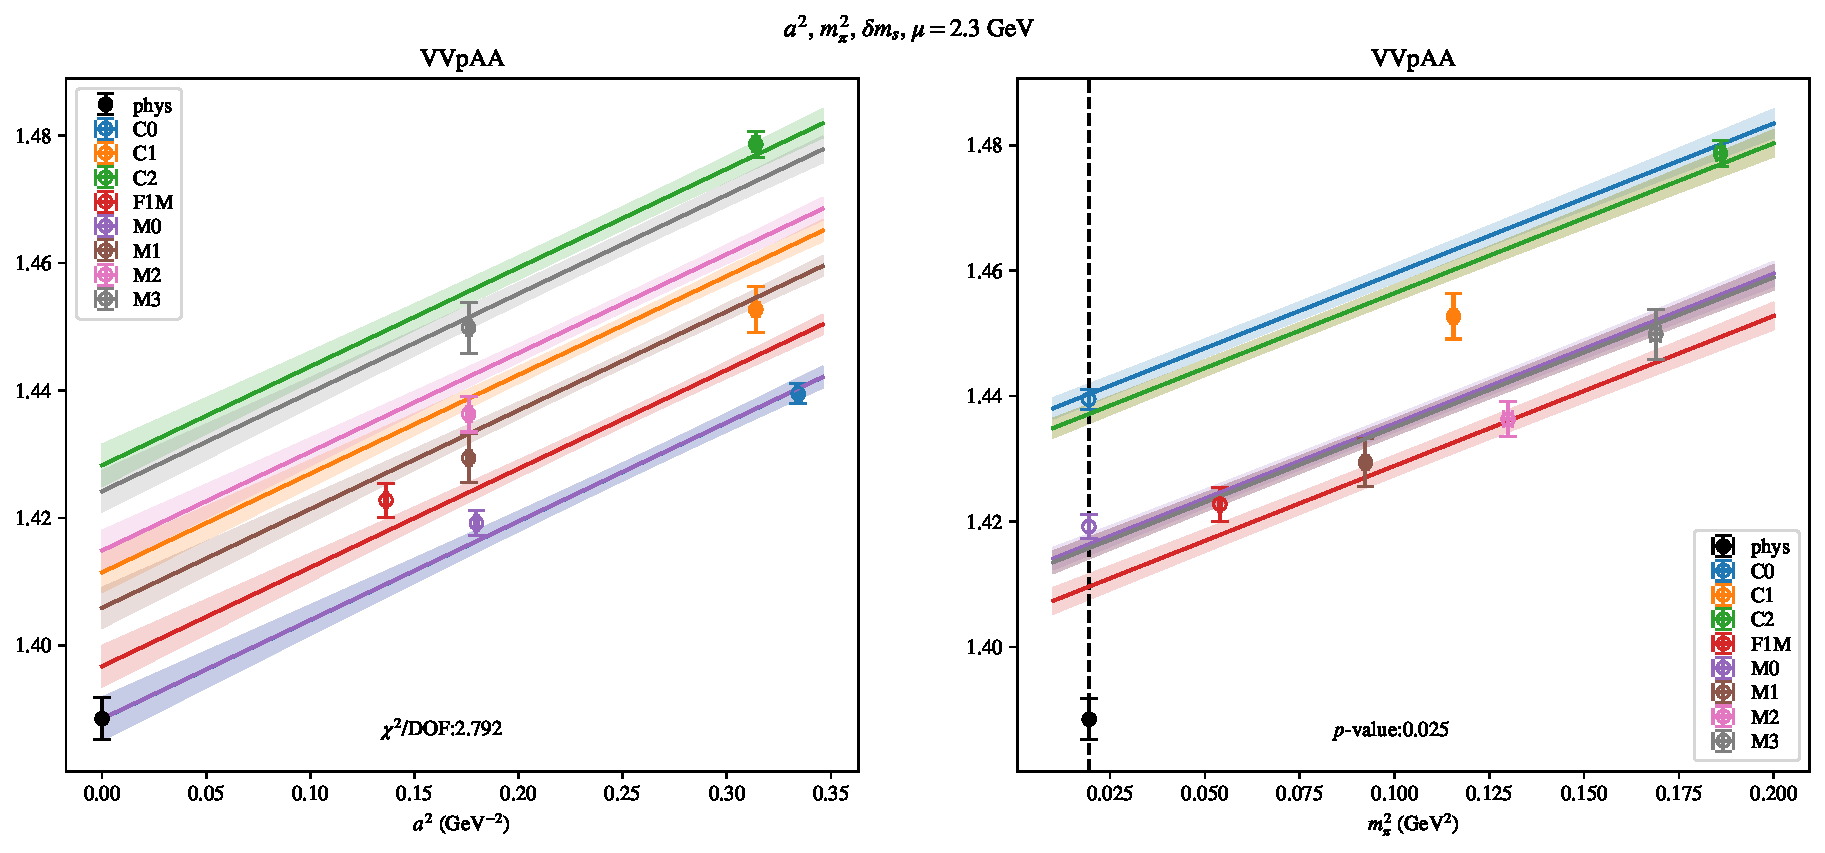
\includepdf[link, pages=-]{VVpAA/SUSY/bag_a2m2delm_23.pdf}
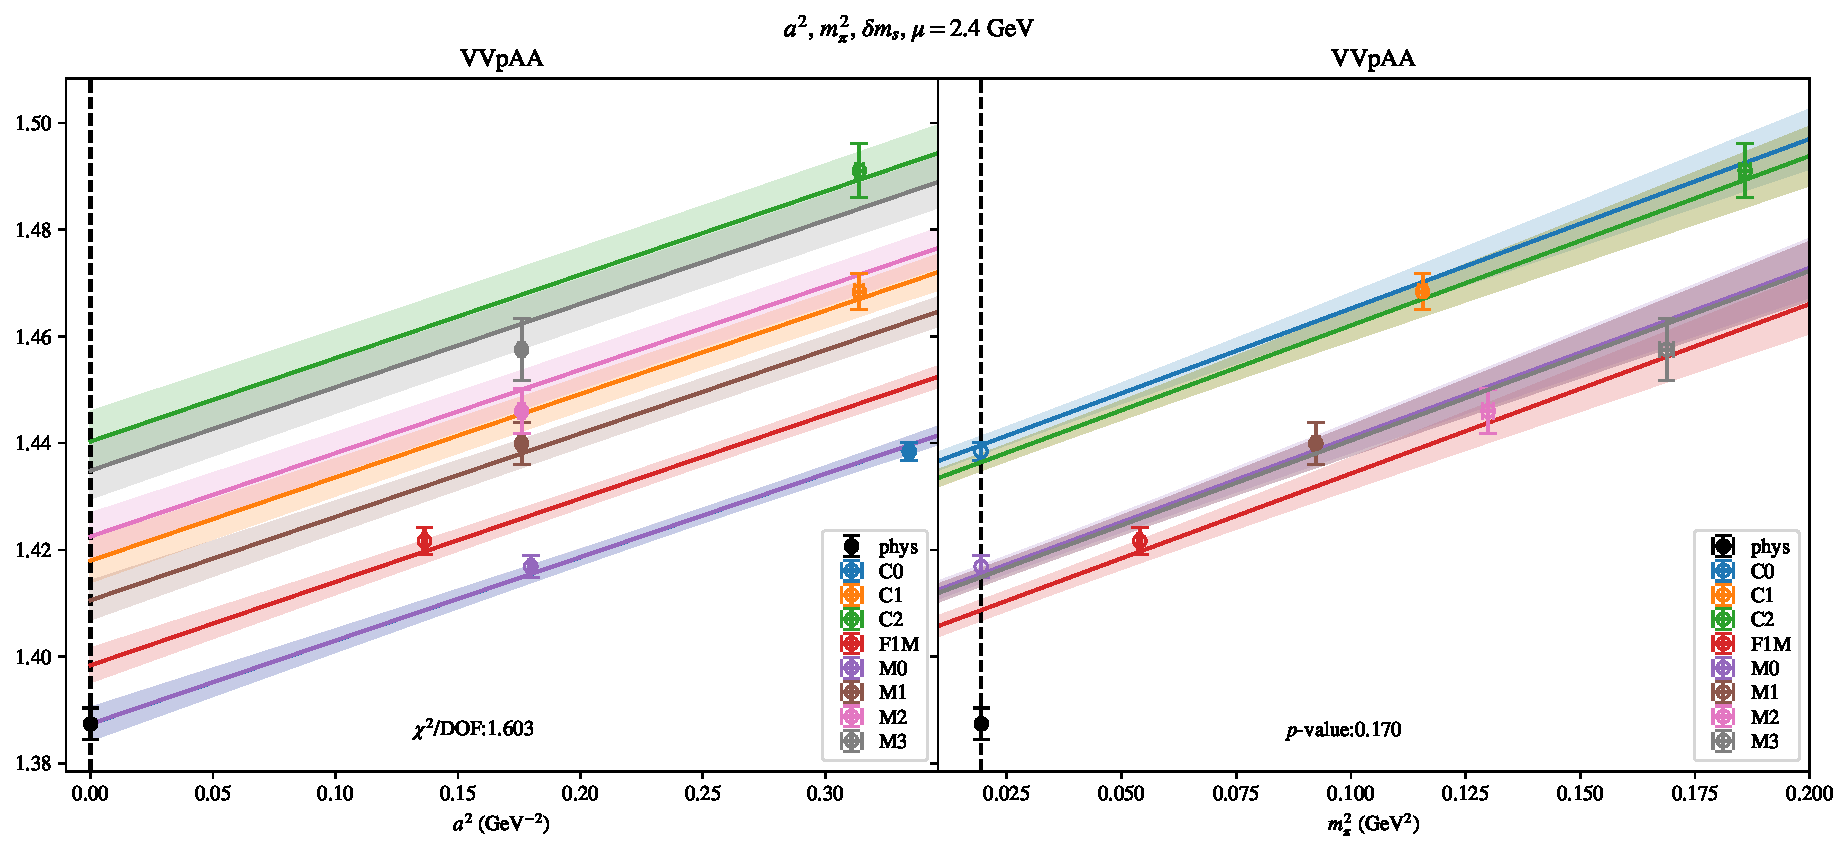
\includepdf[link, pages=-]{VVpAA/SUSY/bag_a2m2delm_24.pdf}
\clearpage
\section{$\mathcal{B}_2$}
\begin{table}[h!]
\begin{center}
\begin{tabular}{|c|c|c|c|c|c|c|}
\hline
$\mu$ (GeV) & $a^2$, $m_\pi^2$& $a^2$, $m_\pi^2$ (no C)& $a^2$, $m_\pi^2$, $a^4$& $a^2$, $m_\pi^2$ (no M3, C2)& $a^2$, $m_\pi^2$, $m_\pi^4$& $a^2$, $m_\pi^2$, $\delta m_s$\\
\hline
2.0& \hyperlink{VVmAA/SUSY/bag_a2m2_20.pdf.1}{\textbf{-0.9261(19)}: 3.557 (0.003)} & \hyperlink{VVmAA/SUSY/bag_a2m2noC_20.pdf.1}{\textbf{-0.9462(79)}: 2.068 (0.126)} & \hyperlink{VVmAA/SUSY/bag_a2a4m2_20.pdf.1}{\textbf{-0.948(13)}: 3.809 (0.004)} & \hyperlink{VVmAA/SUSY/bag_a2m2mcut_20.pdf.1}{\textbf{-0.9254(20)}: 3.893 (0.009)} & \hyperlink{VVmAA/SUSY/bag_a2m2m4_20.pdf.1}{\textbf{-0.9233(21)}: 2.386 (0.049)} & \hyperlink{VVmAA/SUSY/bag_a2m2delm_20.pdf.1}{\textbf{-0.9259(19)}: 4.397 (0.001)}\\
2.2& \hyperlink{VVmAA/SUSY/bag_a2m2_22.pdf.1}{\textbf{-0.9064(18)}: 4.615 (0.0)} & \hyperlink{VVmAA/SUSY/bag_a2m2noC_22.pdf.1}{\textbf{-0.9301(75)}: 1.505 (0.222)} & \hyperlink{VVmAA/SUSY/bag_a2a4m2_22.pdf.1}{\textbf{-0.931(12)}: 4.942 (0.001)} & \hyperlink{VVmAA/SUSY/bag_a2m2mcut_22.pdf.1}{\textbf{-0.9063(19)}: 5.105 (0.002)} & \hyperlink{VVmAA/SUSY/bag_a2m2m4_22.pdf.1}{\textbf{-0.9039(20)}: 3.799 (0.004)} & \hyperlink{VVmAA/SUSY/bag_a2m2delm_22.pdf.1}{\textbf{-0.9064(18)}: 5.789 (0.0)}\\
2.3& \hyperlink{VVmAA/SUSY/bag_a2m2_23.pdf.1}{\textbf{-0.8977(18)}: 5.394 (0.0)} & \hyperlink{VVmAA/SUSY/bag_a2m2noC_23.pdf.1}{\textbf{-0.9227(74)}: 1.87 (0.154)} & \hyperlink{VVmAA/SUSY/bag_a2a4m2_23.pdf.1}{\textbf{-0.924(11)}: 5.653 (0.0)} & \hyperlink{VVmAA/SUSY/bag_a2m2mcut_23.pdf.1}{\textbf{-0.8976(19)}: 6.199 (0.0)} & \hyperlink{VVmAA/SUSY/bag_a2m2m4_23.pdf.1}{\textbf{-0.8951(20)}: 4.424 (0.001)} & \hyperlink{VVmAA/SUSY/bag_a2m2delm_23.pdf.1}{\textbf{-0.8978(18)}: 6.734 (0.0)}\\
2.4& \hyperlink{VVmAA/SUSY/bag_a2m2_24.pdf.1}{\textbf{-0.8898(18)}: 5.818 (0.0)} & \hyperlink{VVmAA/SUSY/bag_a2m2noC_24.pdf.1}{\textbf{-0.9154(73)}: 1.971 (0.139)} & \hyperlink{VVmAA/SUSY/bag_a2a4m2_24.pdf.1}{\textbf{-0.917(11)}: 6.081 (0.0)} & \hyperlink{VVmAA/SUSY/bag_a2m2mcut_24.pdf.1}{\textbf{-0.8897(19)}: 7.112 (0.0)} & \hyperlink{VVmAA/SUSY/bag_a2m2m4_24.pdf.1}{\textbf{-0.8872(20)}: 5.136 (0.0)} & \hyperlink{VVmAA/SUSY/bag_a2m2delm_24.pdf.1}{\textbf{-0.8899(17)}: 7.349 (0.0)}\\
\hline
\end{tabular}
\caption{Physical point value from chiral and continuum extrapolation at renormalisation scale $\mu$. Entries are \textbf{value(error)}: $\chi^2/\text{DOF}$ ($p$-value).}
\end{center}
\end{table}
\begin{table}[h!]
\begin{center}
\begin{tabular}{|c c|c|c|c|c|c|c|}
\hline
$\mu$ (GeV) &  & $a^2$, $m_\pi^2$& $a^2$, $m_\pi^2$ (no C)& $a^2$, $m_\pi^2$, $a^4$& $a^2$, $m_\pi^2$ (no M3, C2)& $a^2$, $m_\pi^2$, $m_\pi^4$& $a^2$, $m_\pi^2$, $\delta m_s$\\
\hline
\multirow{3}{0.5in}{2.0} & $\alpha$ & -0.3483(74)& -0.232(45)& -0.15(11)& -0.3499(79)& -0.3570(79)& -0.3492(74)\\
 & $\beta$ & -0.00625(16)& -0.00587(30)& -0.00633(16)& -0.00669(26)& -0.00859(85)& -0.00629(32)\\
 & $\gamma$ &  &  & -0.40(24)&  & 0.000214(76)& 0.001(11)\\
\hline
\multirow{3}{0.5in}{2.2} & $\alpha$ & -0.3830(71)& -0.247(44)& -0.16(11)& -0.3824(75)& -0.3904(75)& -0.3833(71)\\
 & $\beta$ & -0.00651(15)& -0.00595(28)& -0.00659(15)& -0.00693(25)& -0.00866(78)& -0.00663(29)\\
 & $\gamma$ &  &  & -0.46(22)&  & 0.000197(70)& 0.005(10)\\
\hline
\multirow{3}{0.5in}{2.3} & $\alpha$ & -0.3985(69)& -0.256(43)& -0.16(10)& -0.3980(74)& -0.4067(75)& -0.3989(70)\\
 & $\beta$ & -0.00651(14)& -0.00600(26)& -0.00662(15)& -0.00693(24)& -0.00877(76)& -0.00662(29)\\
 & $\gamma$ &  &  & -0.49(22)&  & 0.000207(68)& 0.004(10)\\
\hline
\multirow{3}{0.5in}{2.4} & $\alpha$ & -0.4131(69)& -0.267(42)& -0.17(10)& -0.4125(74)& -0.4211(74)& -0.4132(68)\\
 & $\beta$ & -0.00653(14)& -0.00601(25)& -0.00664(15)& -0.00690(23)& -0.00870(74)& -0.00666(29)\\
 & $\gamma$ &  &  & -0.50(22)&  & 0.000199(67)& 0.005(10)\\
\hline
\end{tabular}
\caption{Fit values of coefficients in $Q = Q_{phys} + \mathbf{\alpha} a^2 + \mathbf{\beta}\left(\frac{m_\pi^2}{f_\pi^2}-\frac{m_{\pi,PDG}^2}{f_\pi^2}\right) + \gamma(\ldots)$}
\end{center}
\end{table}
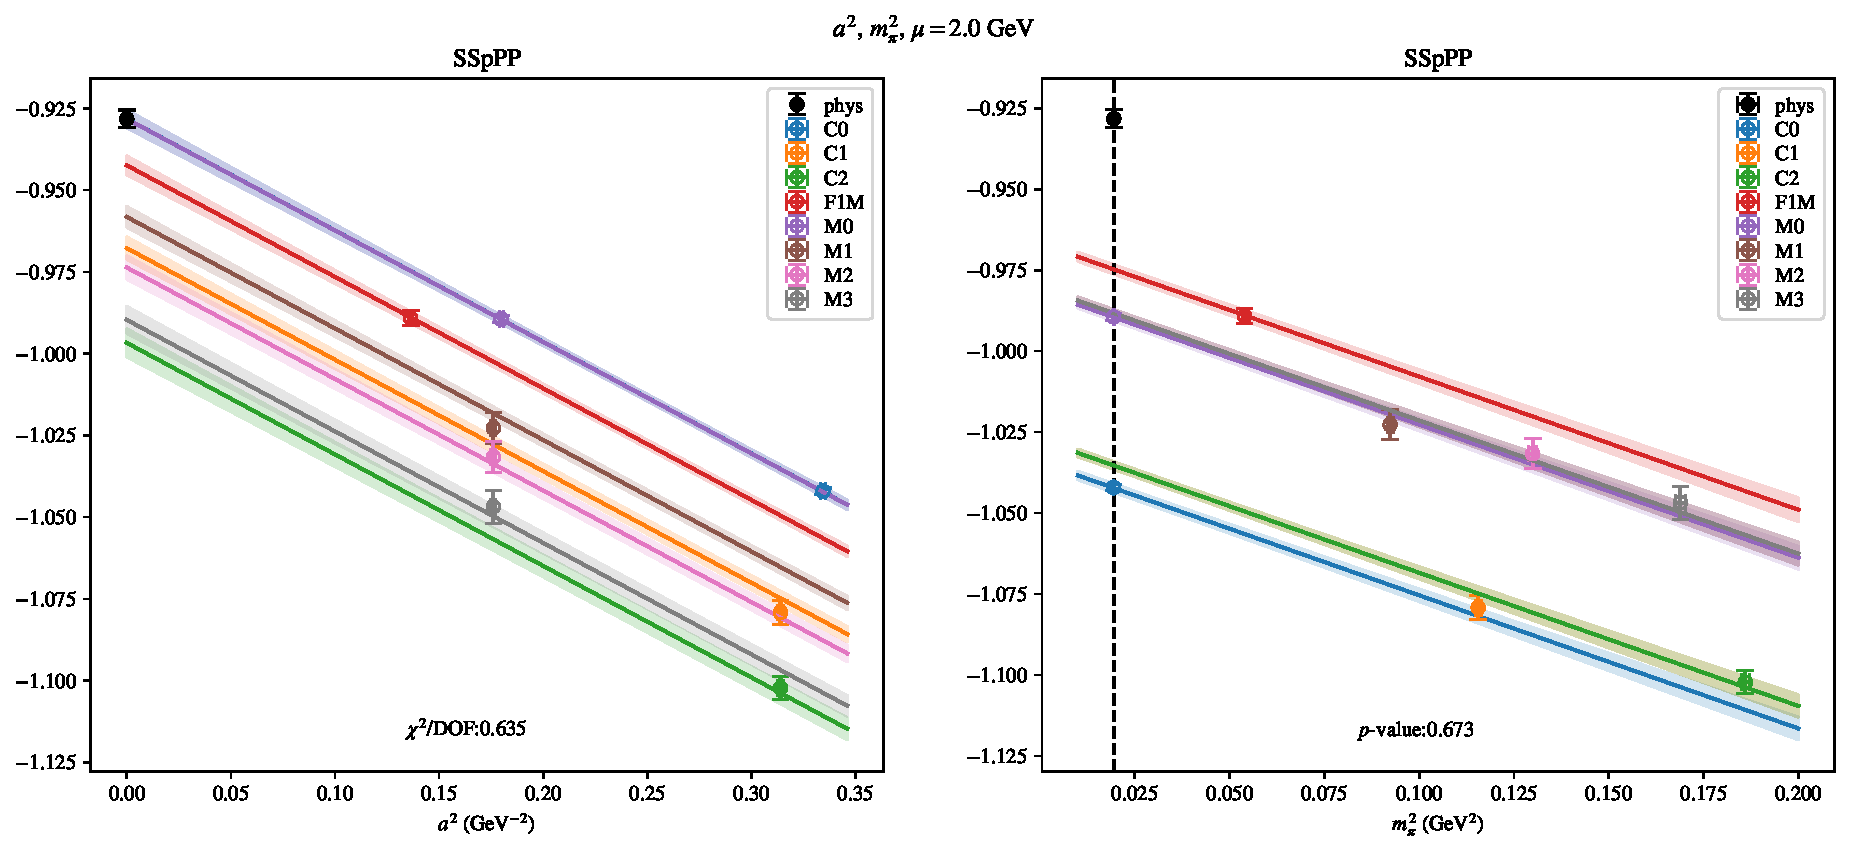
\includepdf[link, pages=-]{VVmAA/SUSY/bag_a2m2_20.pdf}
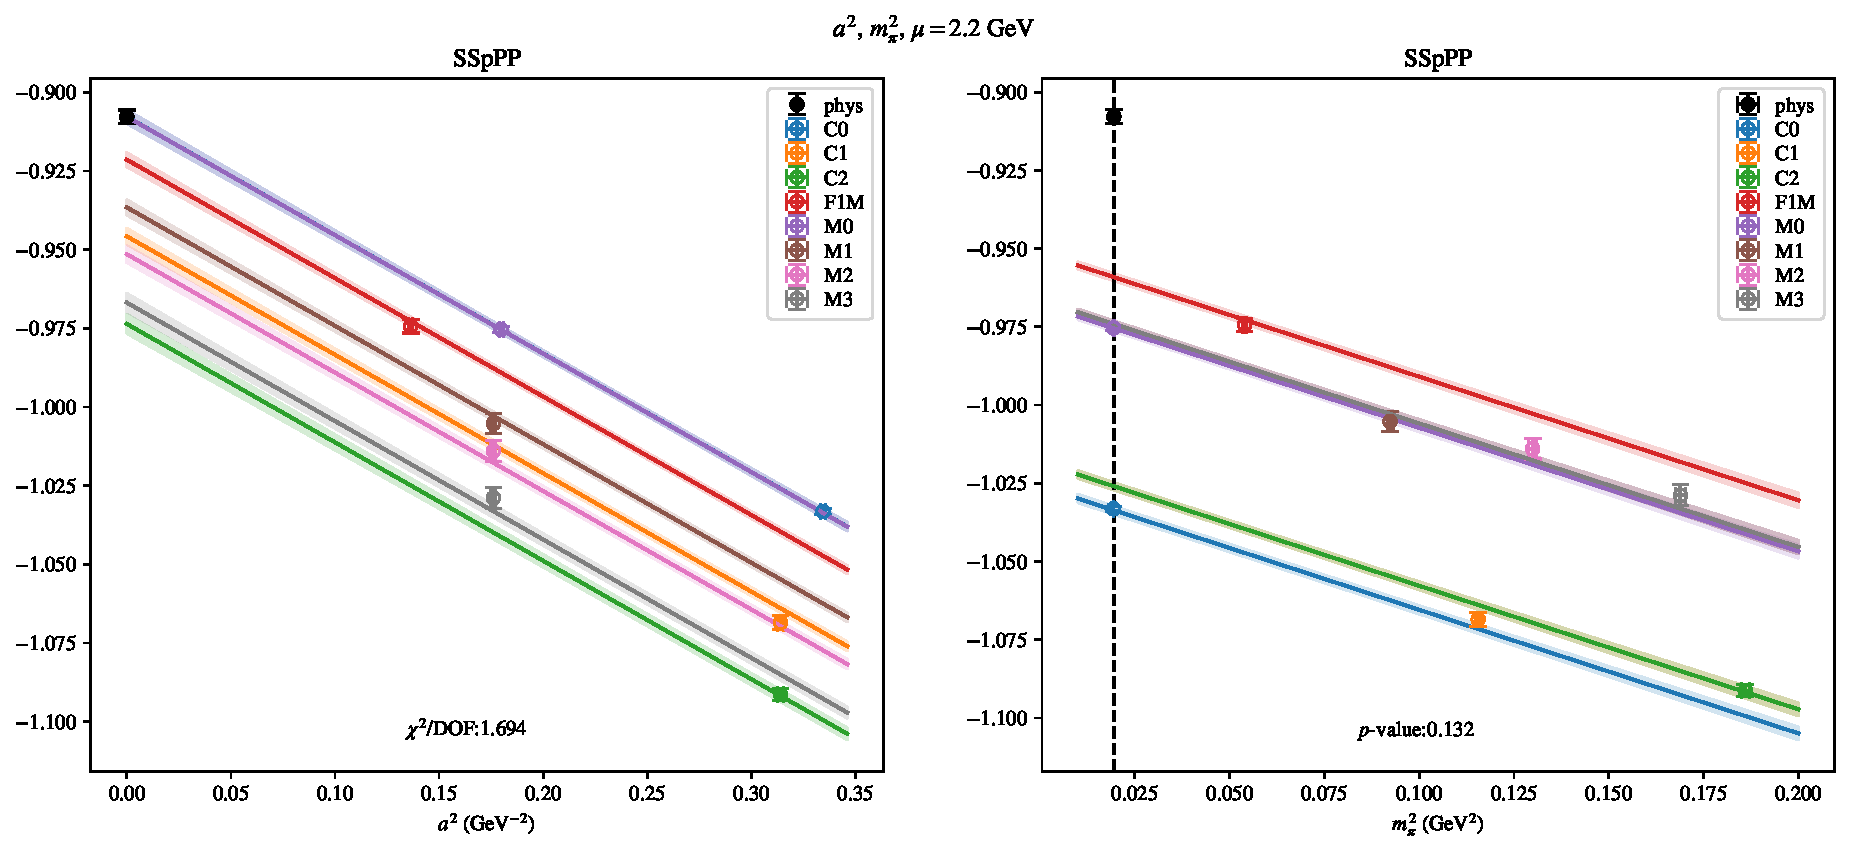
\includepdf[link, pages=-]{VVmAA/SUSY/bag_a2m2_22.pdf}
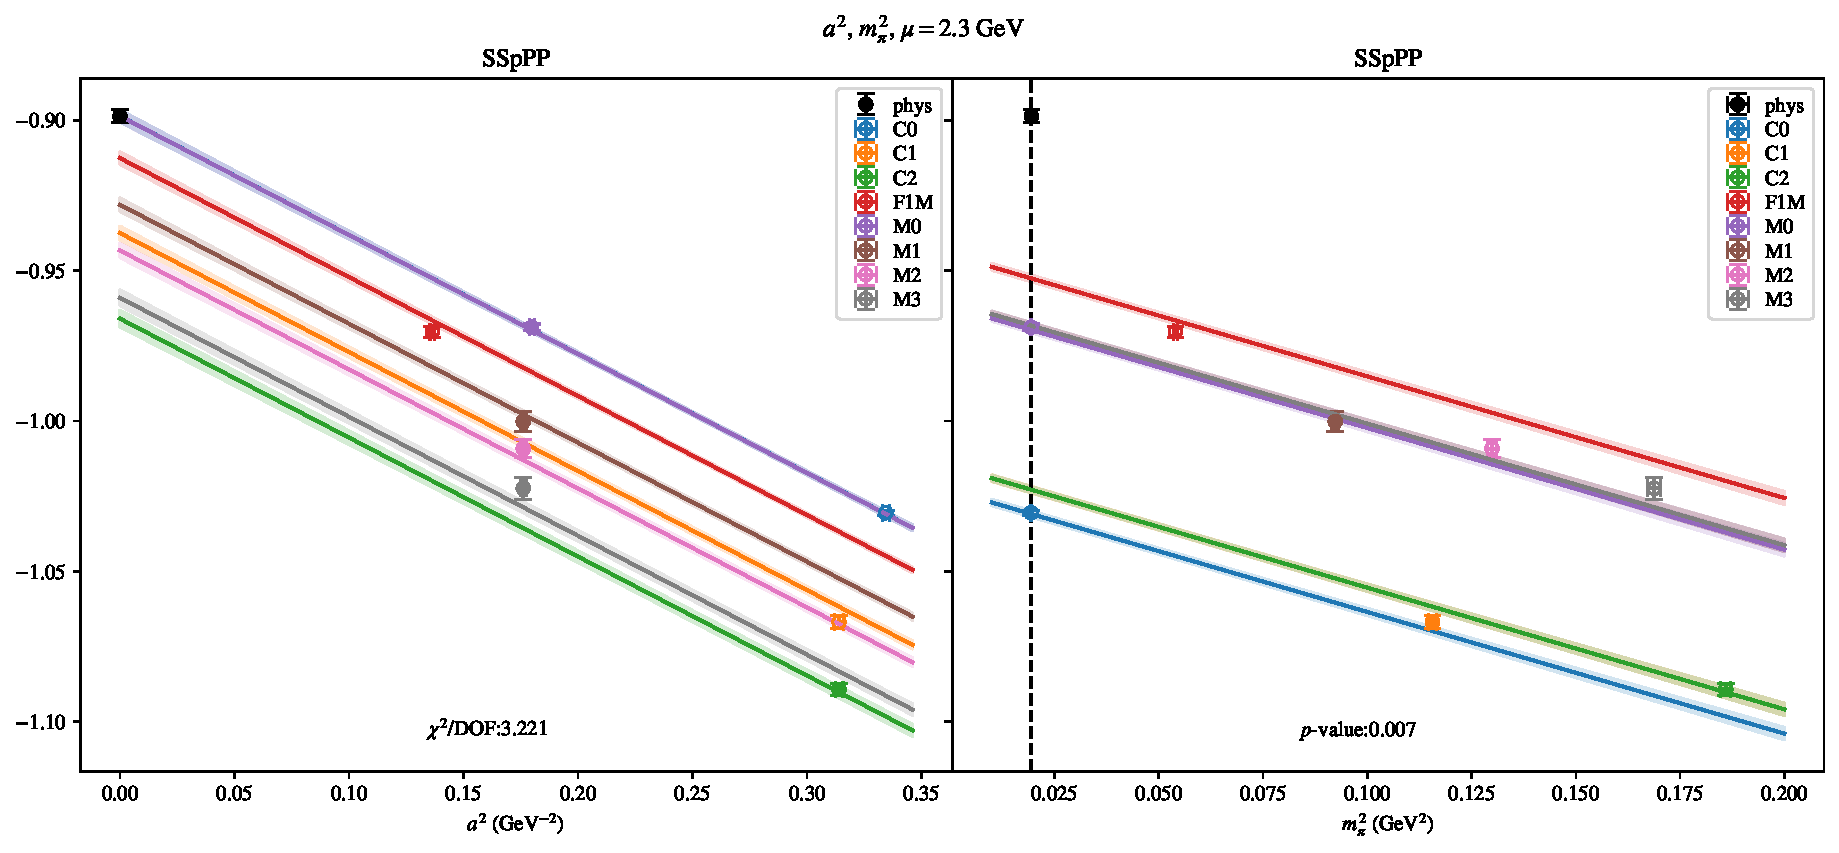
\includepdf[link, pages=-]{VVmAA/SUSY/bag_a2m2_23.pdf}
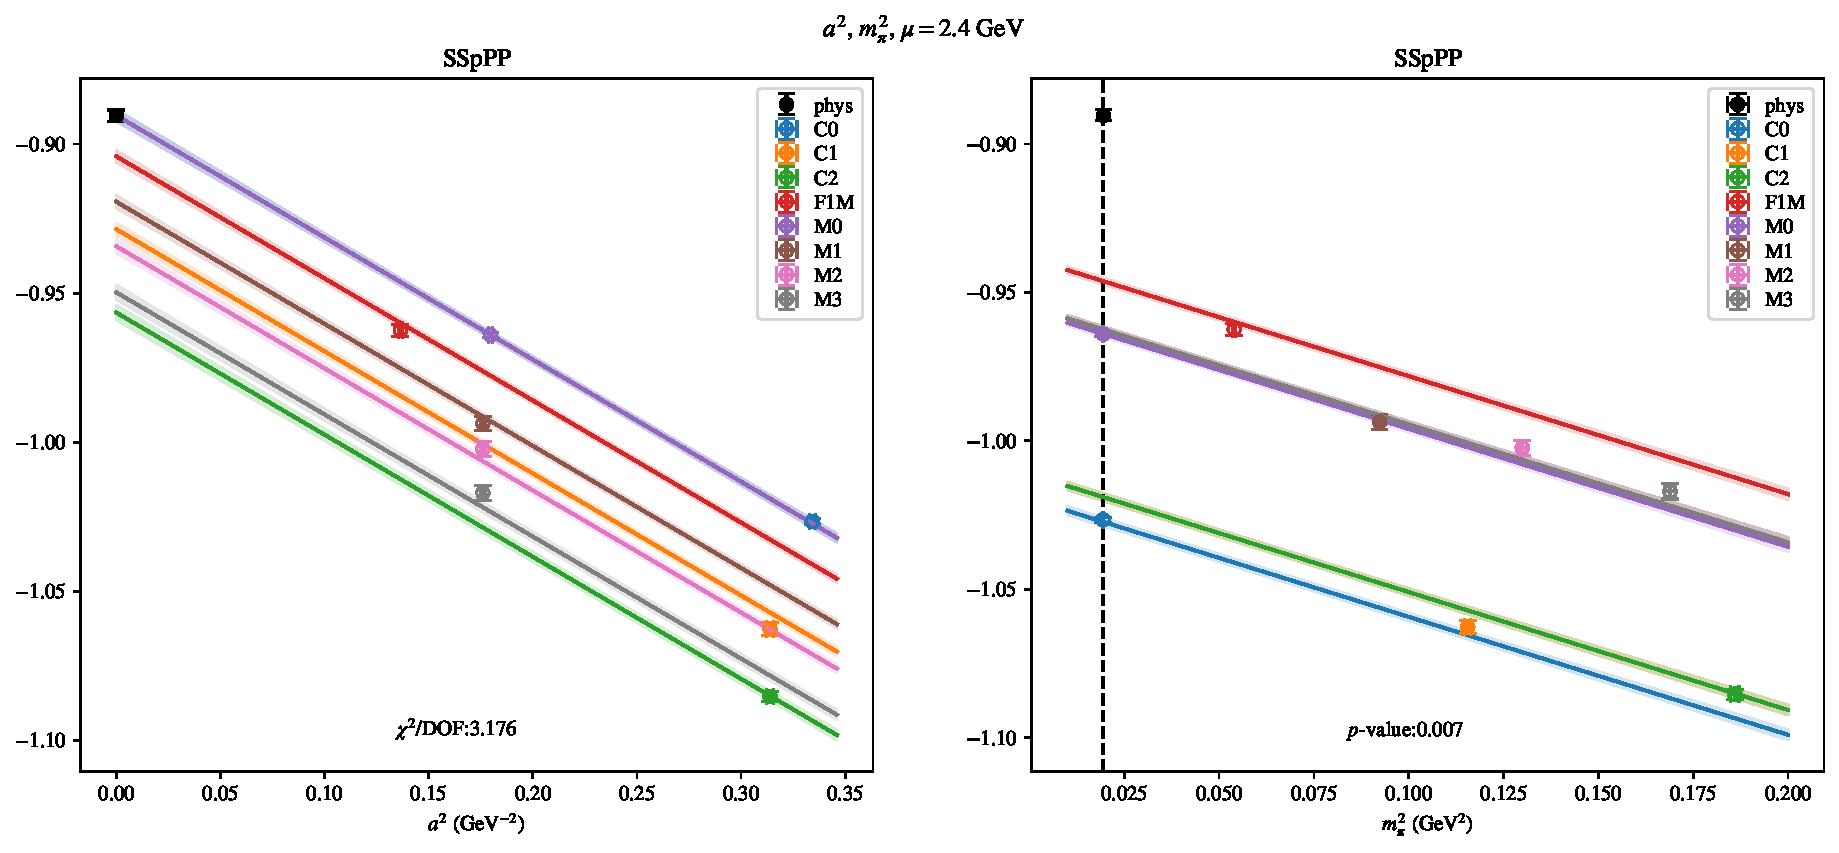
\includepdf[link, pages=-]{VVmAA/SUSY/bag_a2m2_24.pdf}
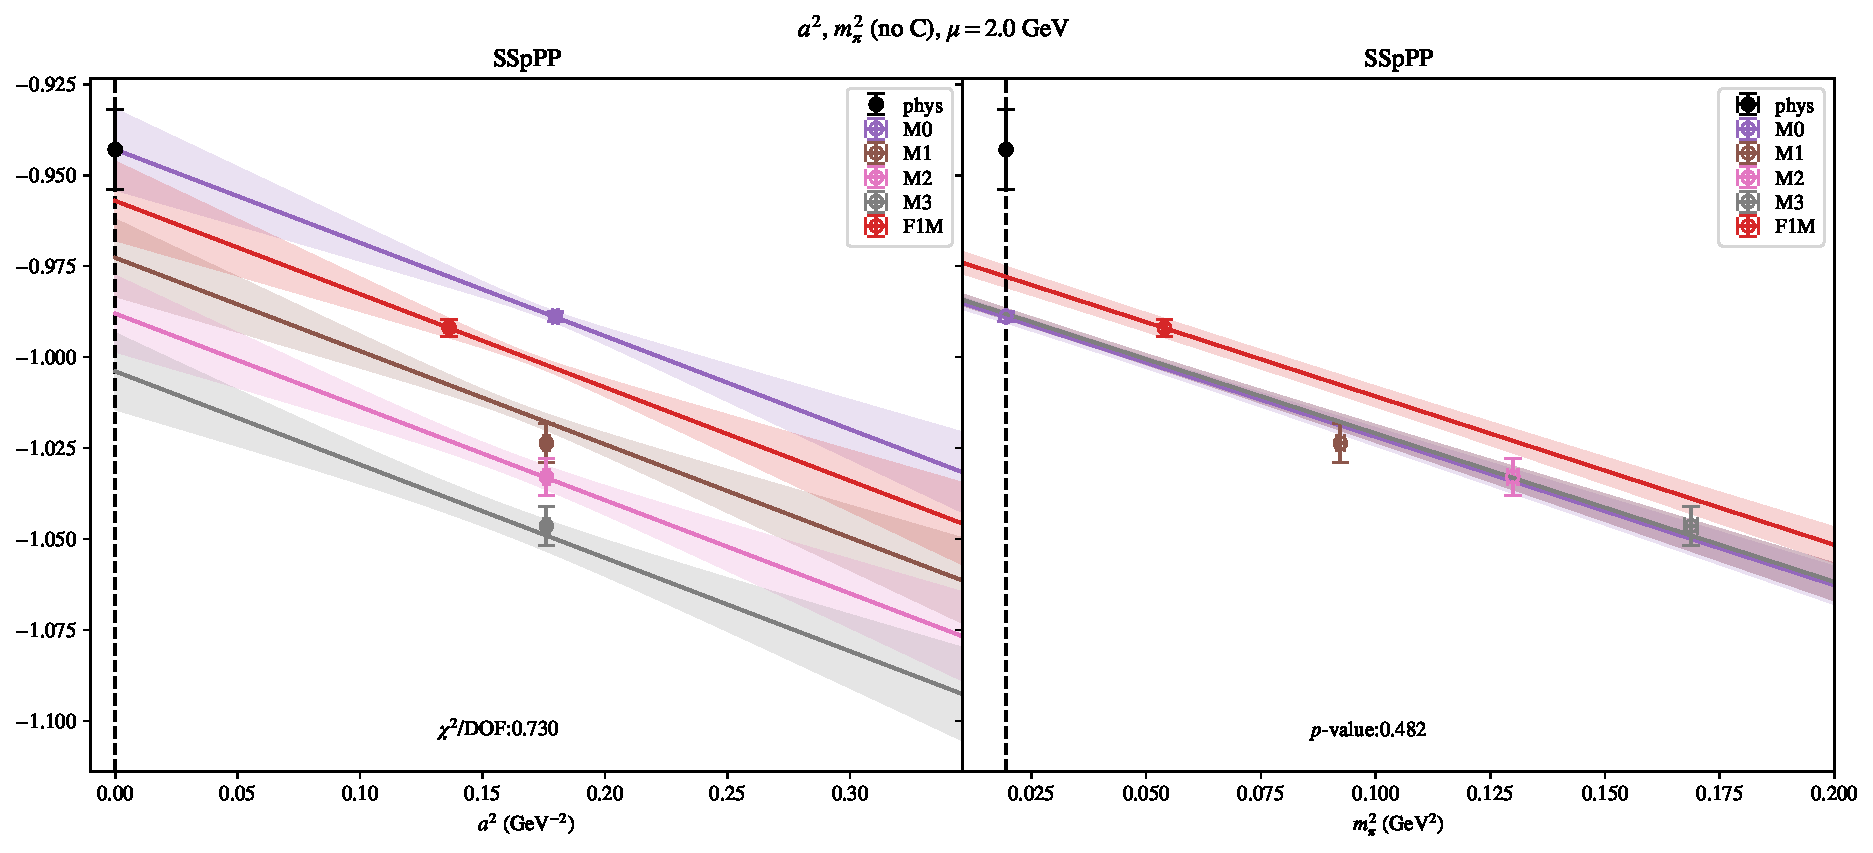
\includepdf[link, pages=-]{VVmAA/SUSY/bag_a2m2noC_20.pdf}
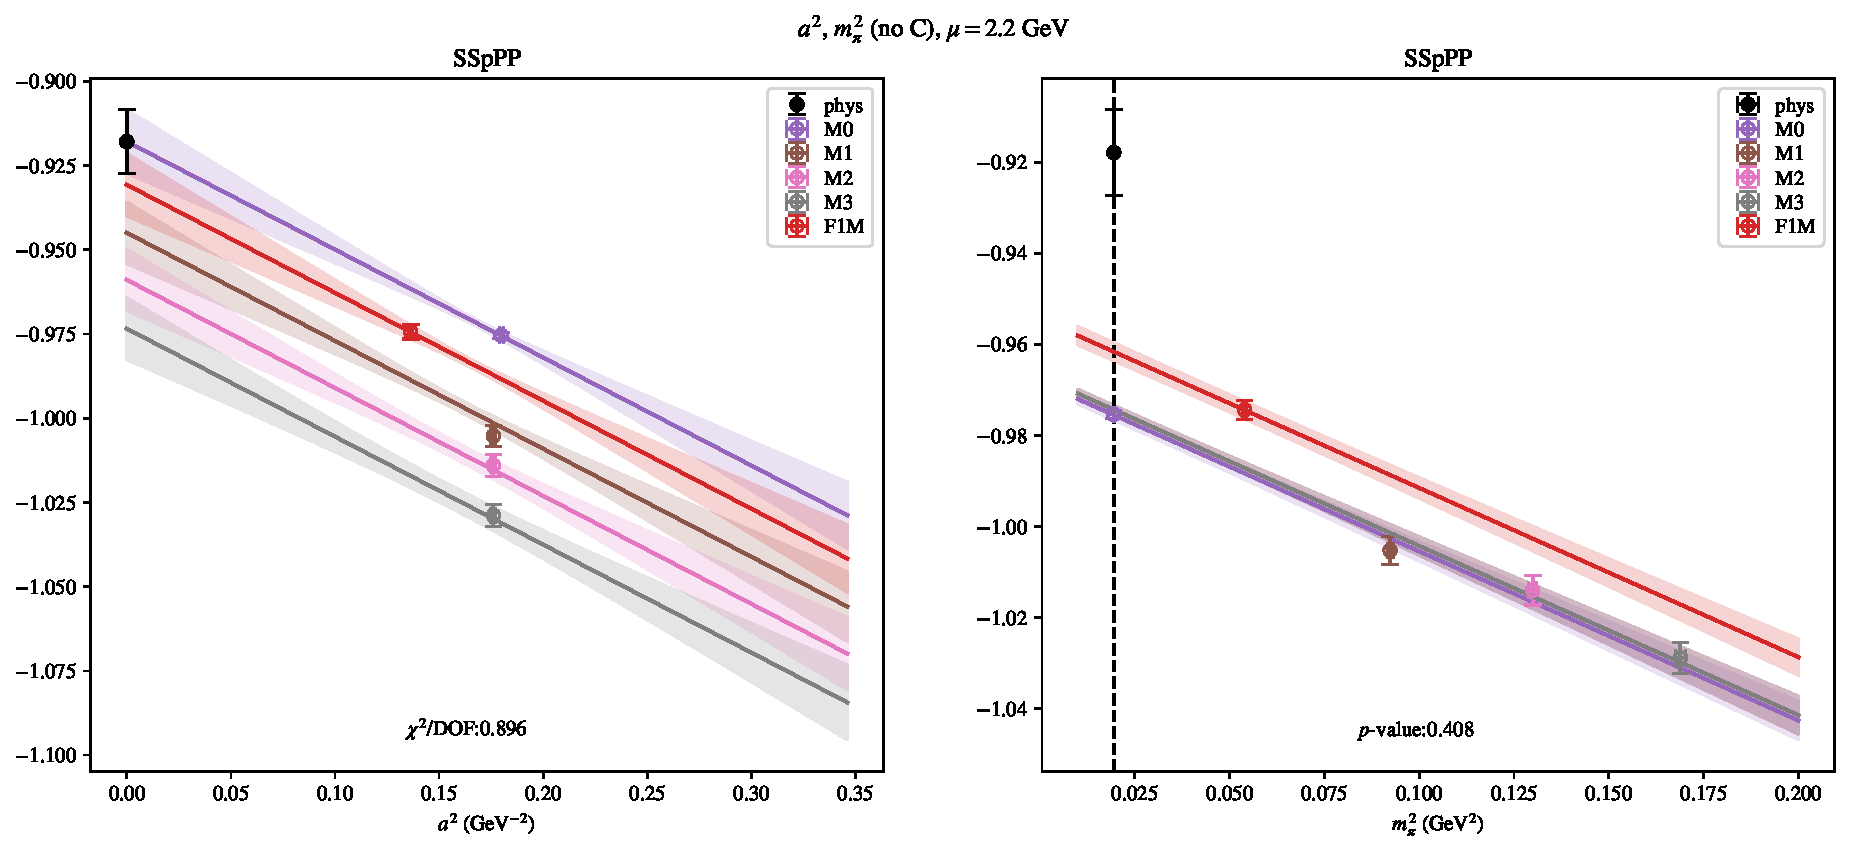
\includepdf[link, pages=-]{VVmAA/SUSY/bag_a2m2noC_22.pdf}
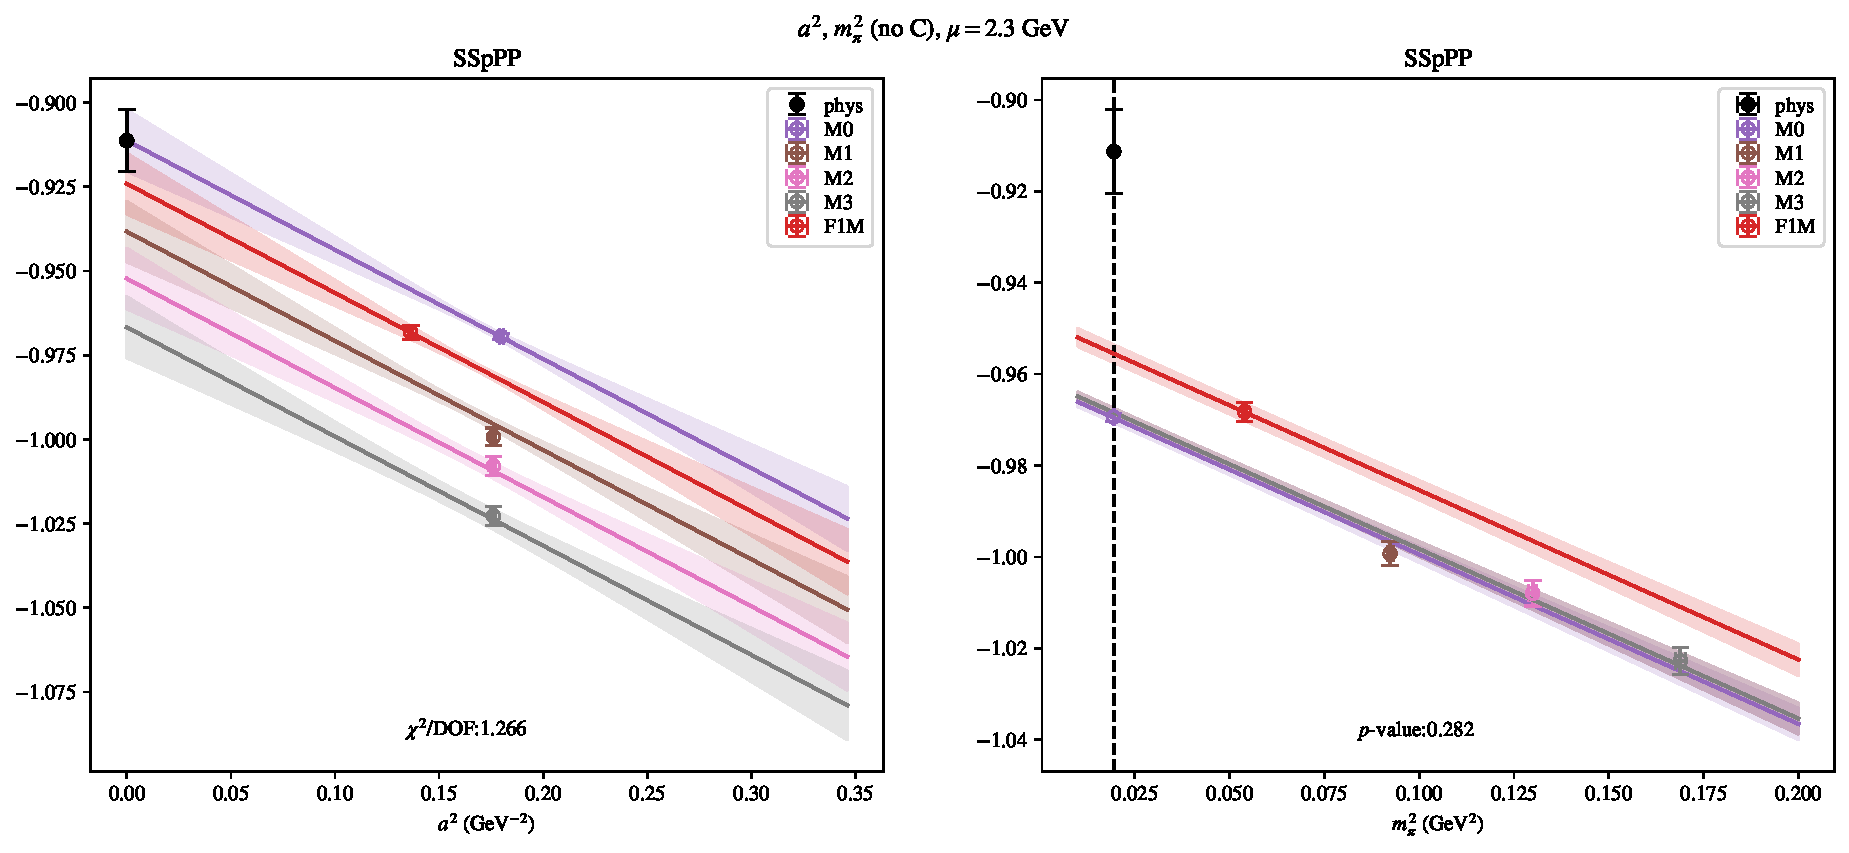
\includepdf[link, pages=-]{VVmAA/SUSY/bag_a2m2noC_23.pdf}
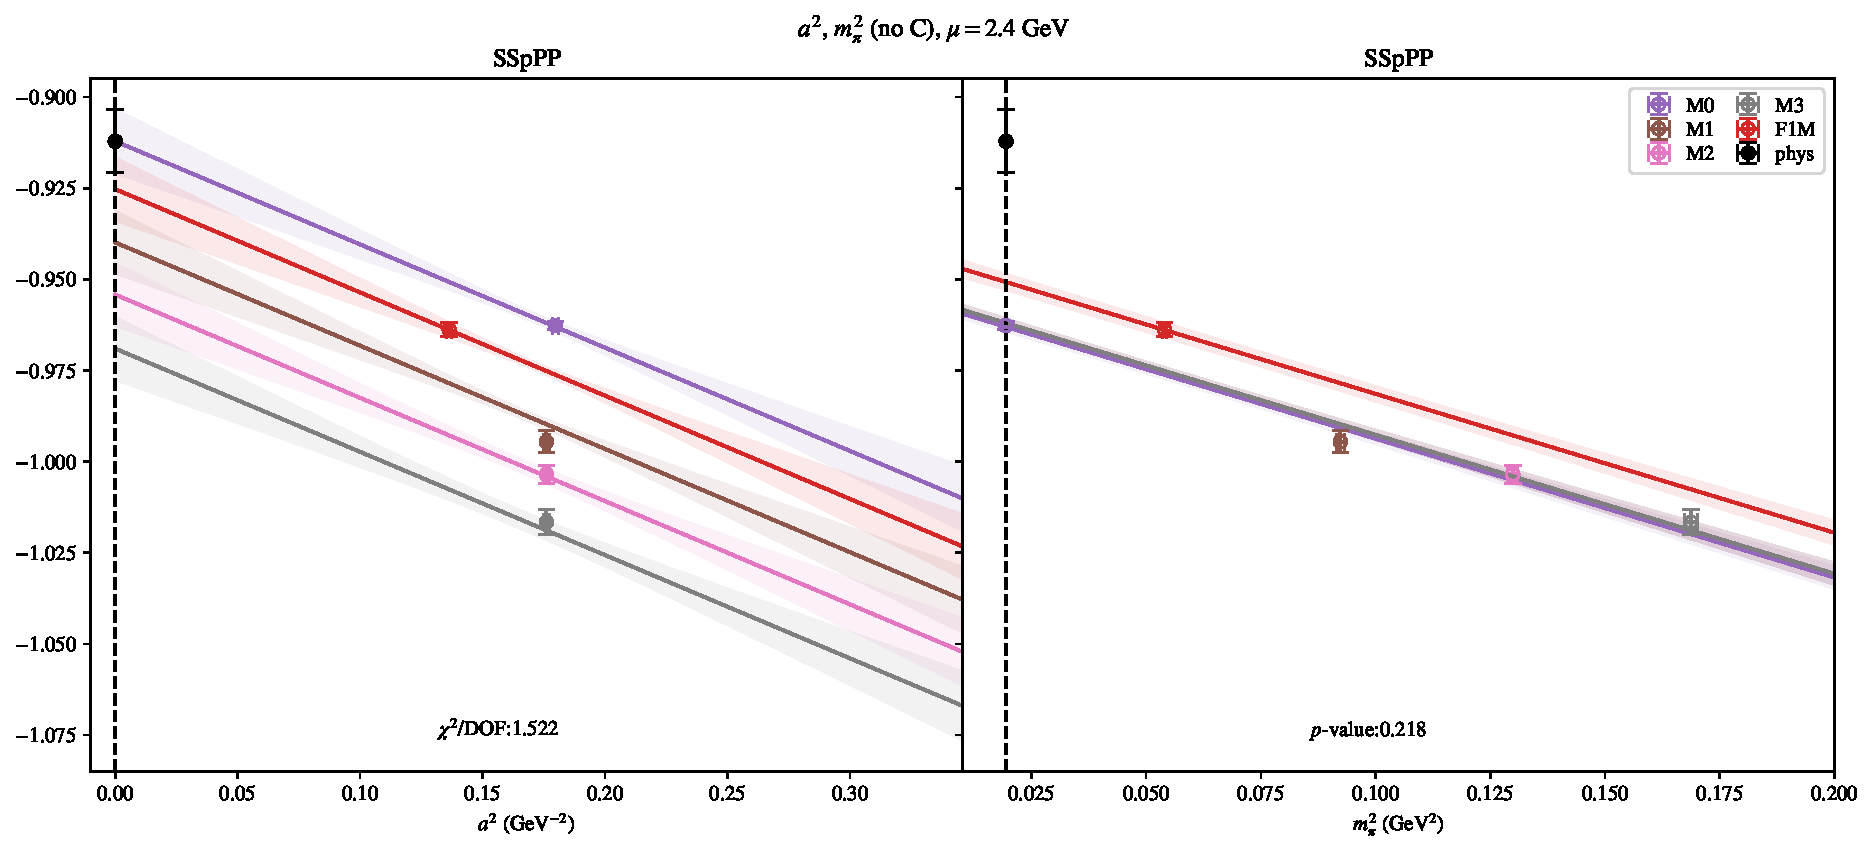
\includepdf[link, pages=-]{VVmAA/SUSY/bag_a2m2noC_24.pdf}
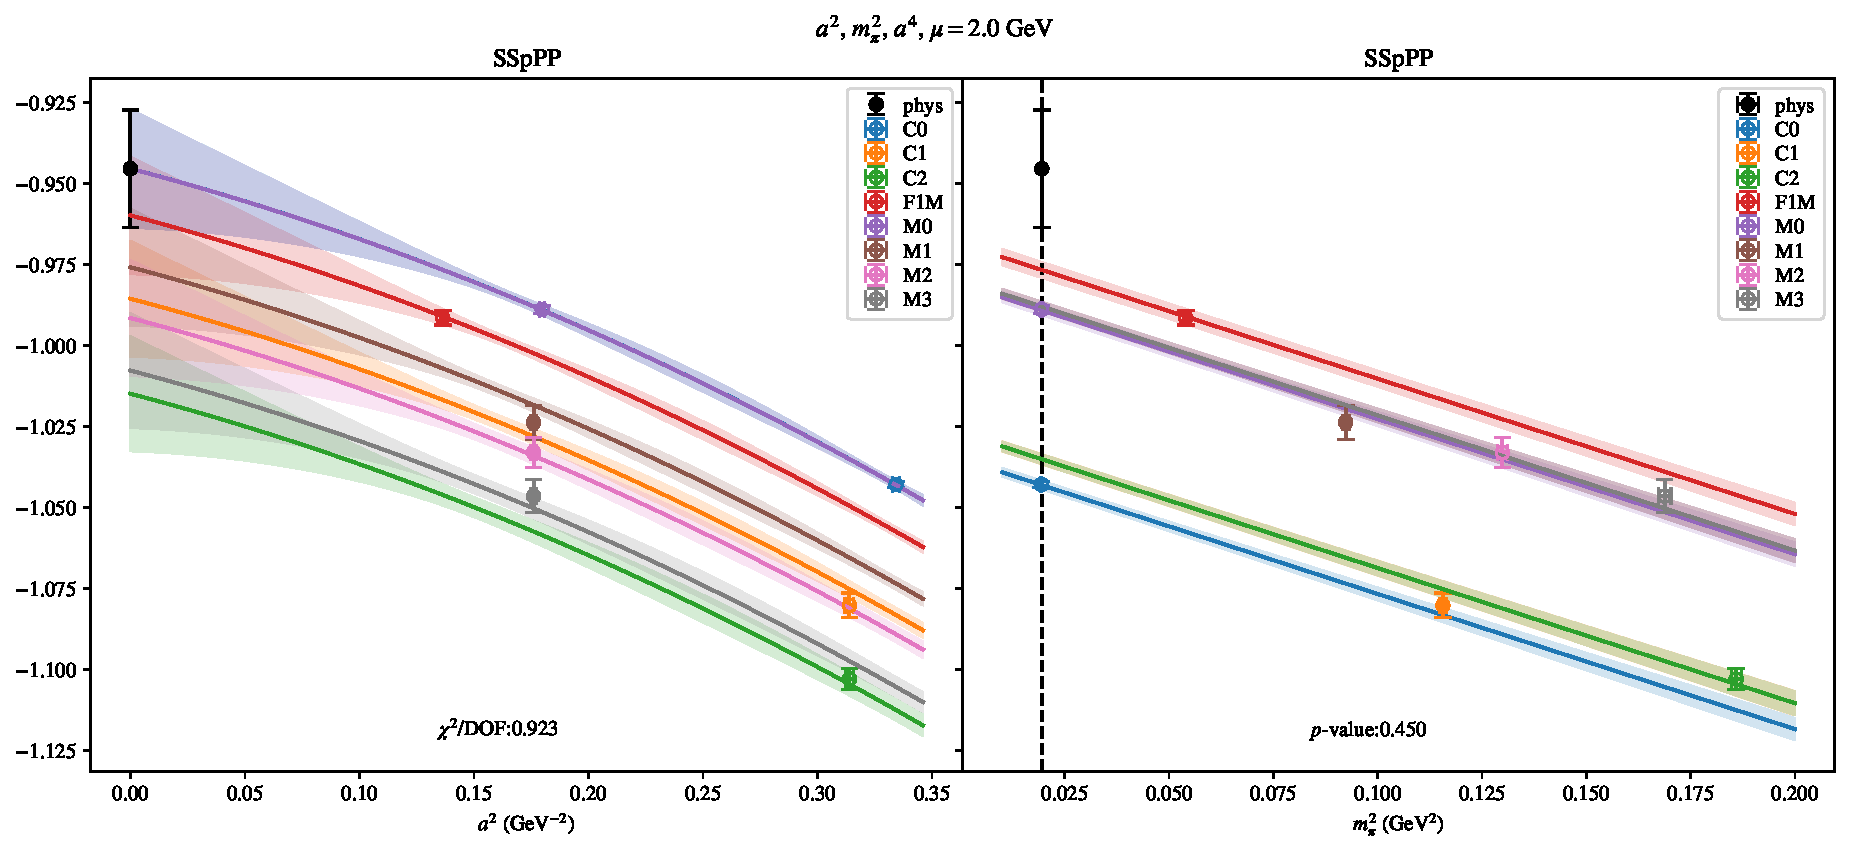
\includepdf[link, pages=-]{VVmAA/SUSY/bag_a2a4m2_20.pdf}
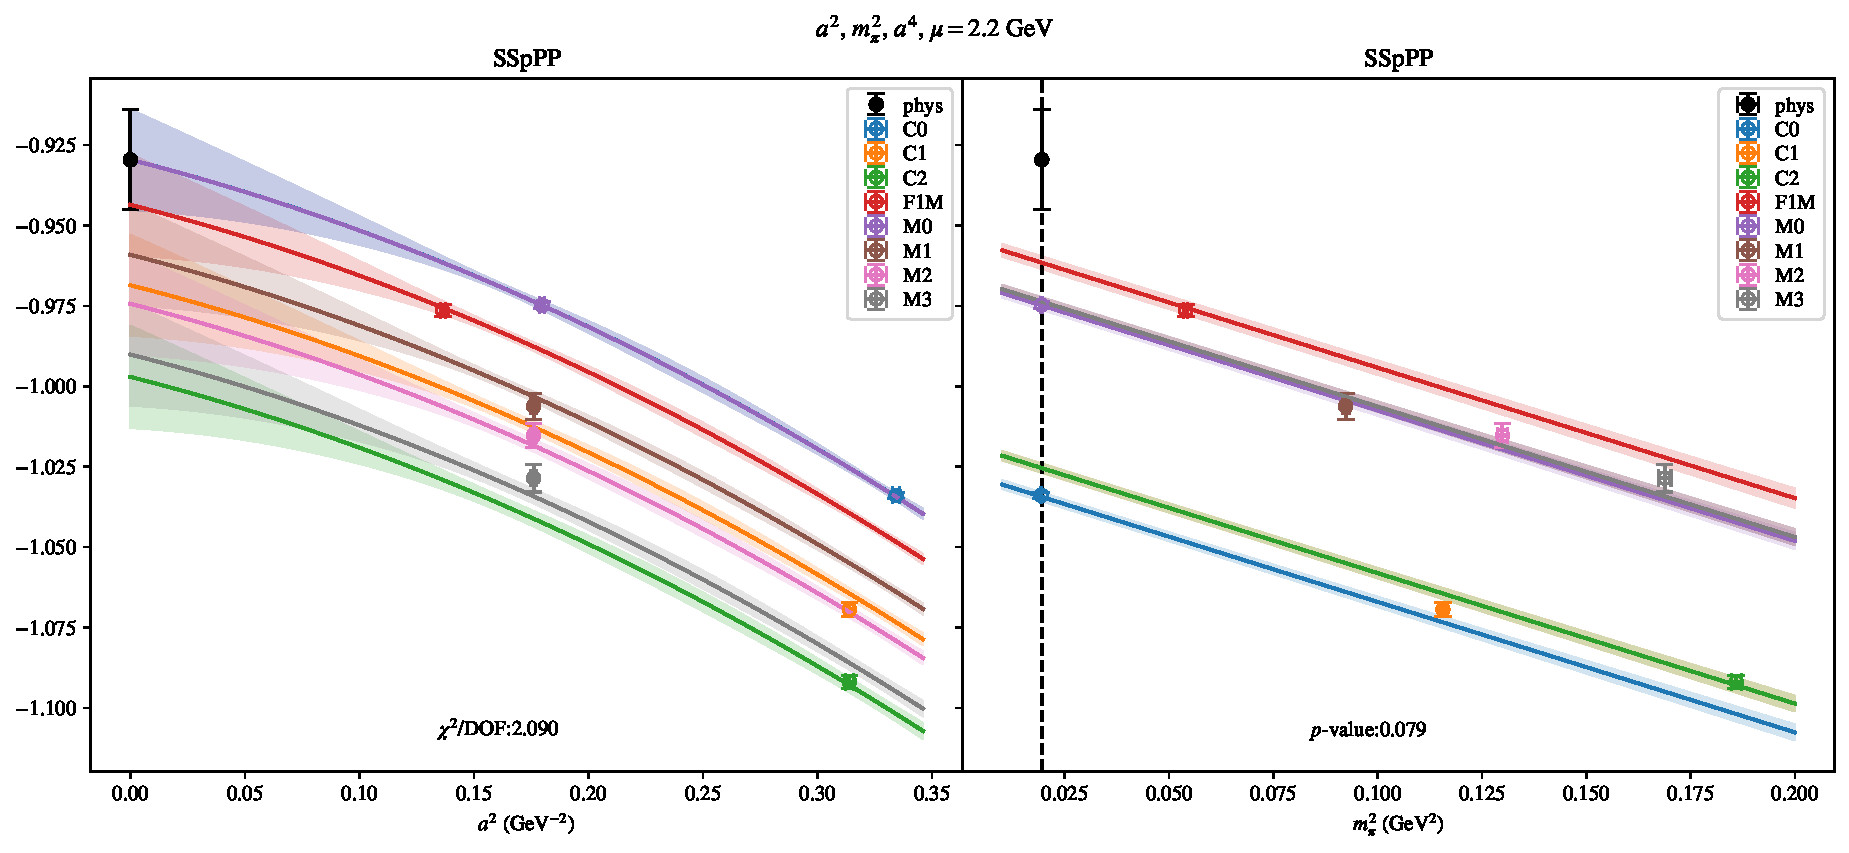
\includepdf[link, pages=-]{VVmAA/SUSY/bag_a2a4m2_22.pdf}
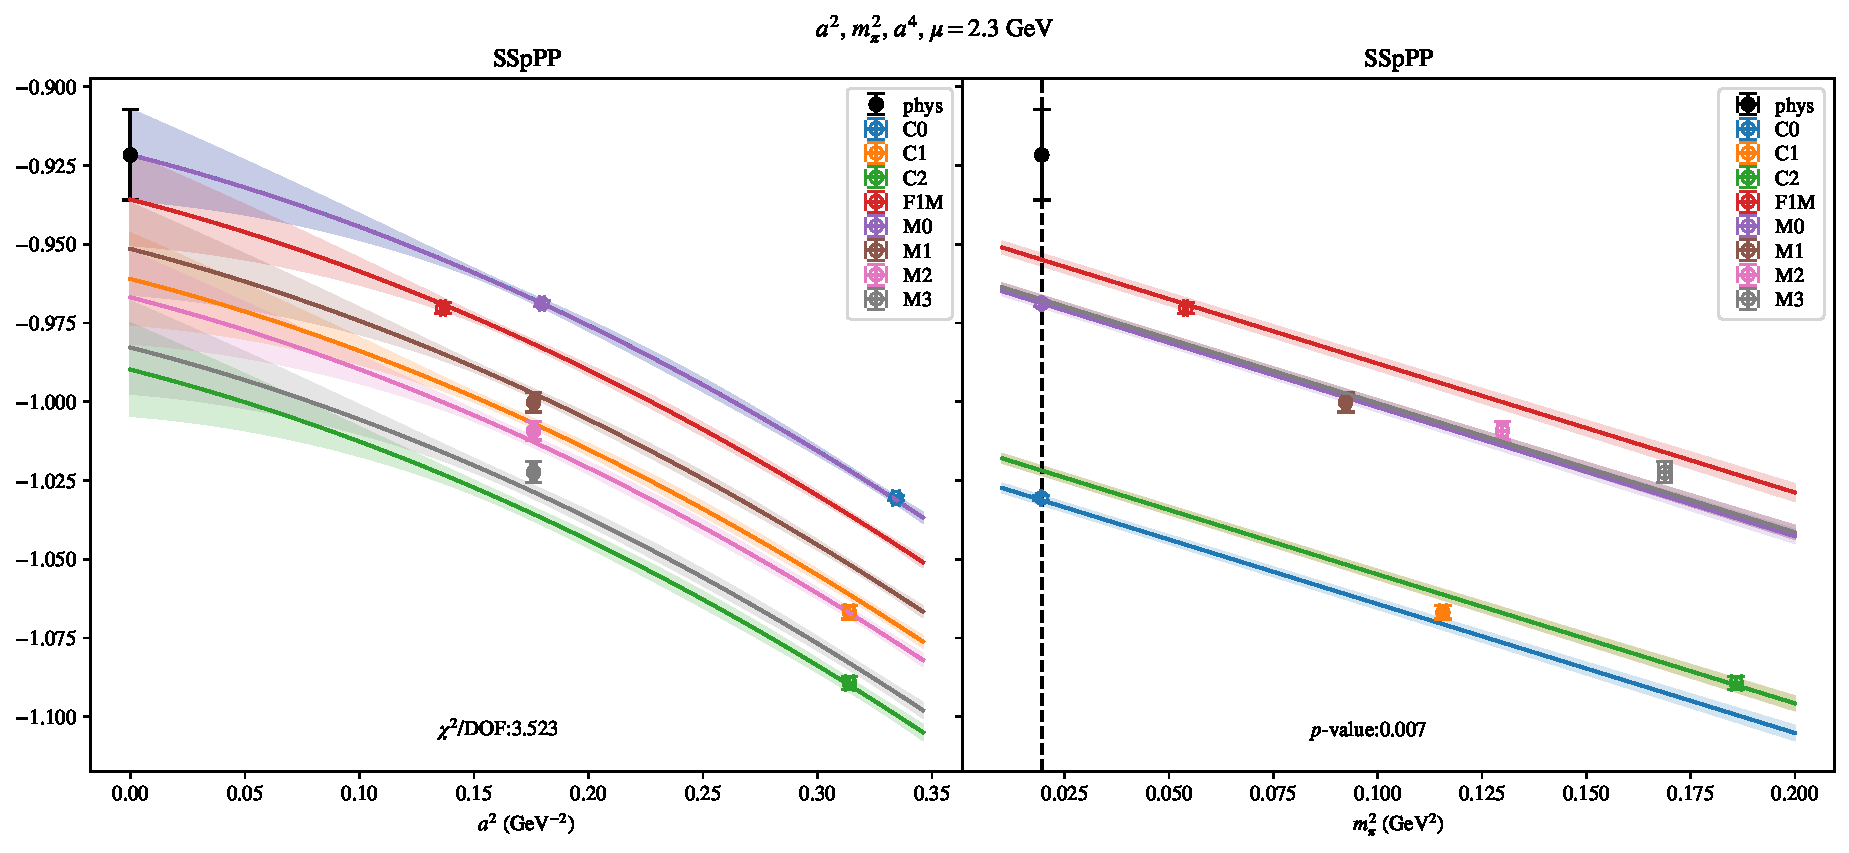
\includepdf[link, pages=-]{VVmAA/SUSY/bag_a2a4m2_23.pdf}
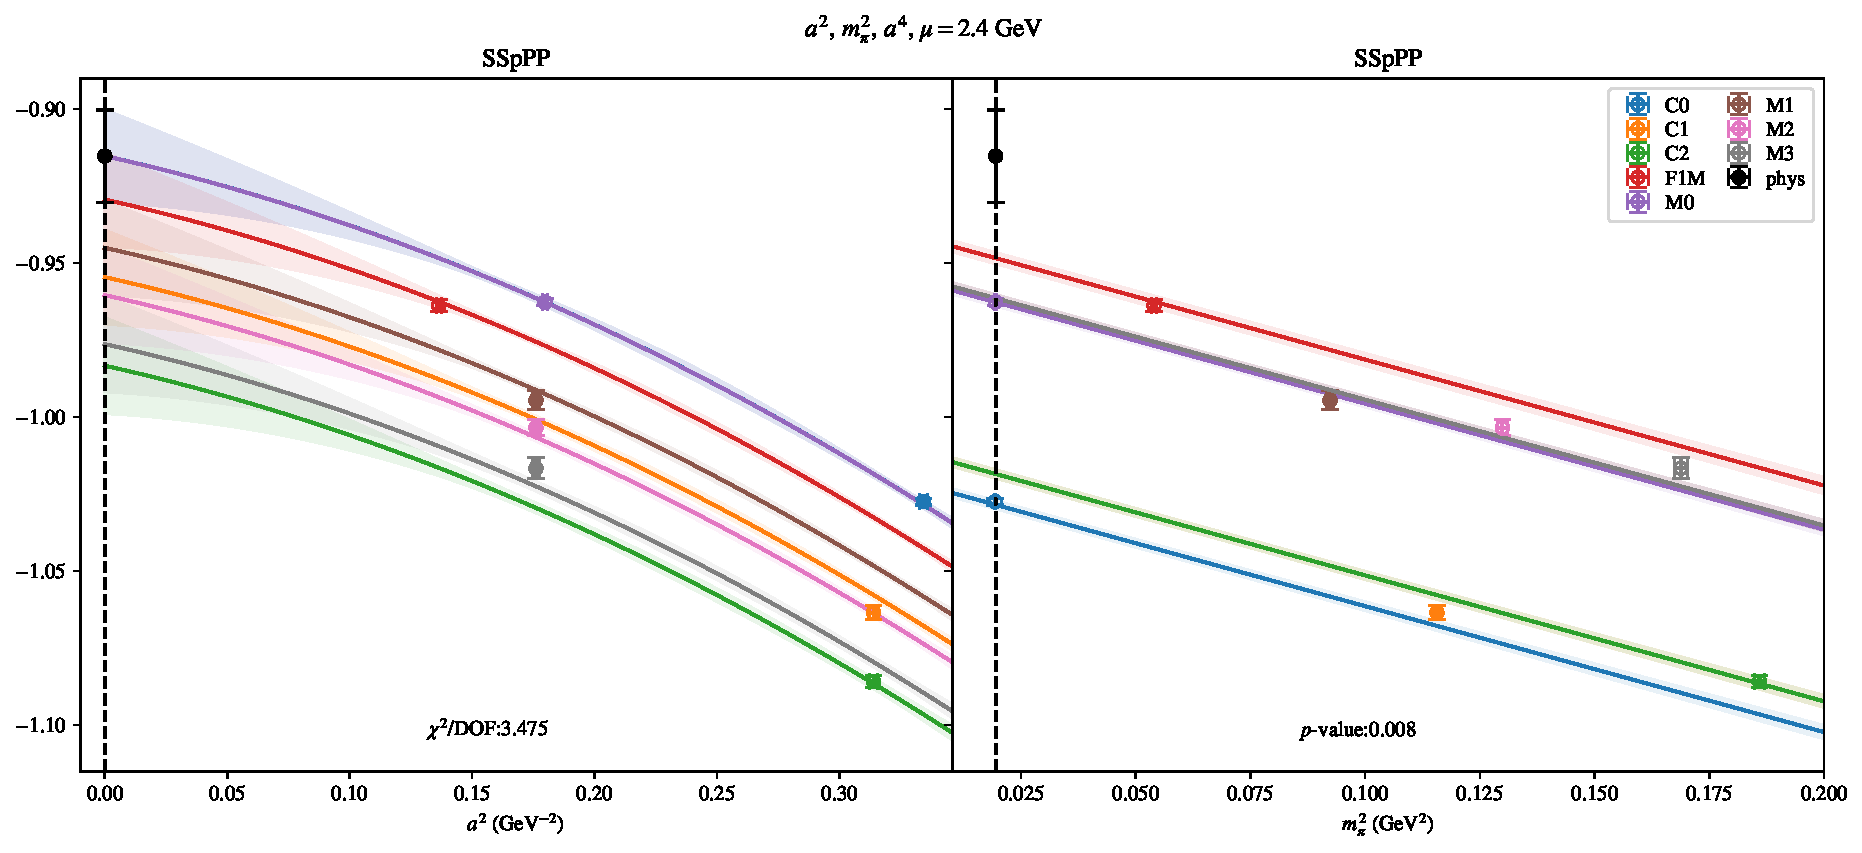
\includepdf[link, pages=-]{VVmAA/SUSY/bag_a2a4m2_24.pdf}
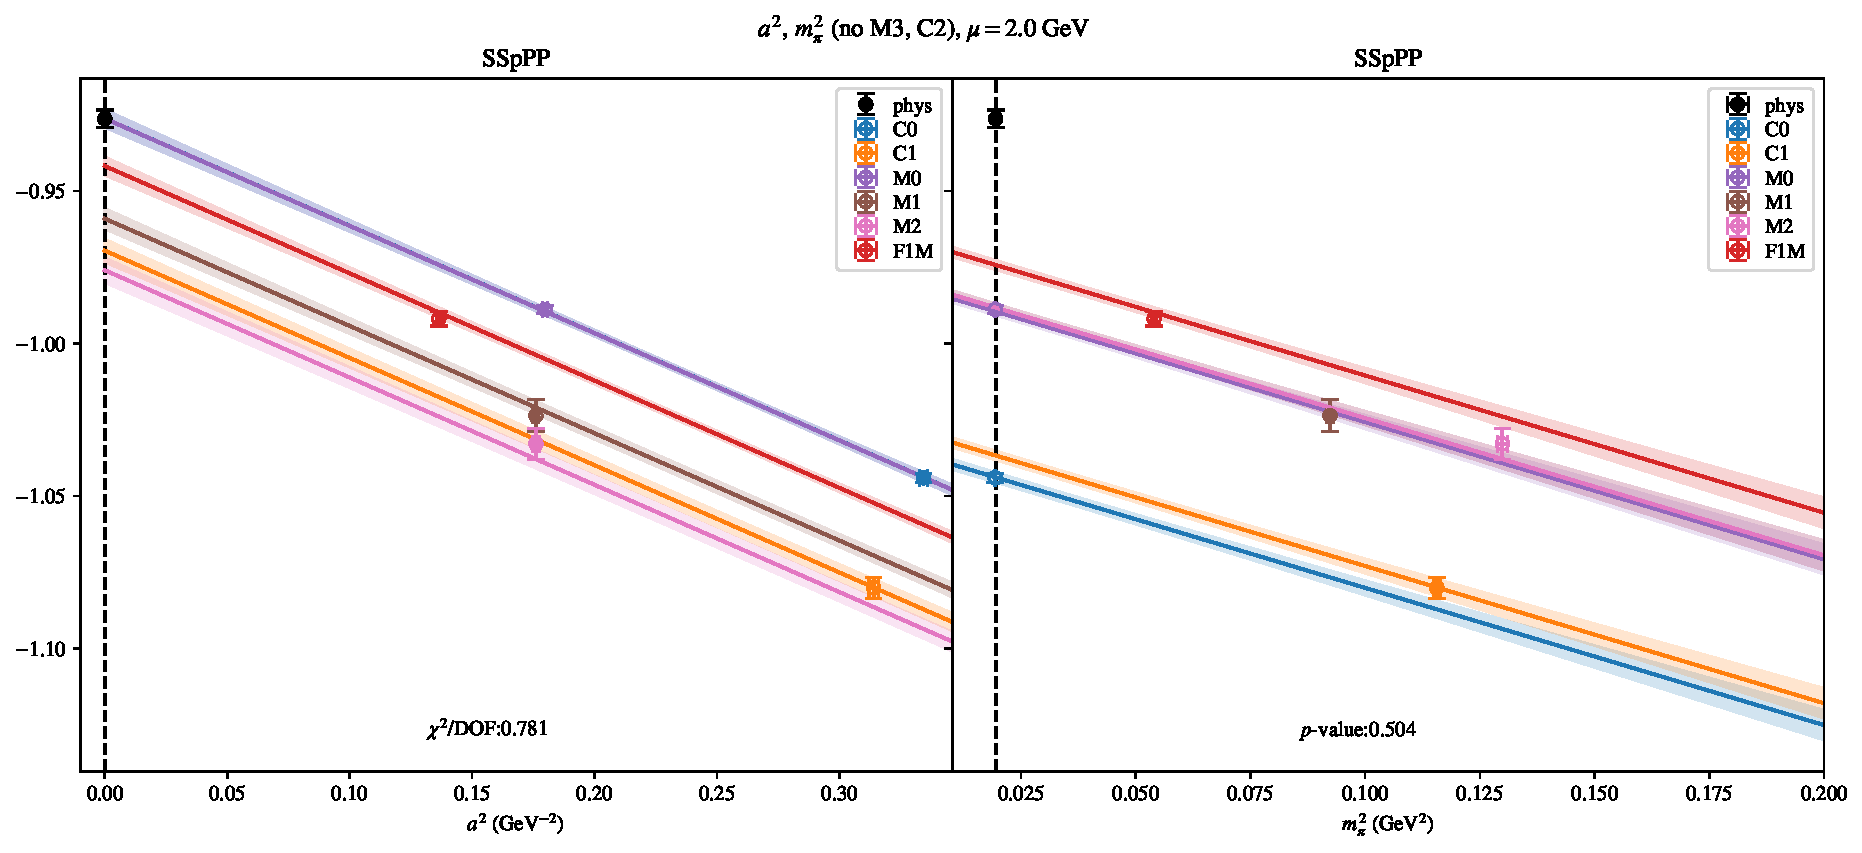
\includepdf[link, pages=-]{VVmAA/SUSY/bag_a2m2mcut_20.pdf}
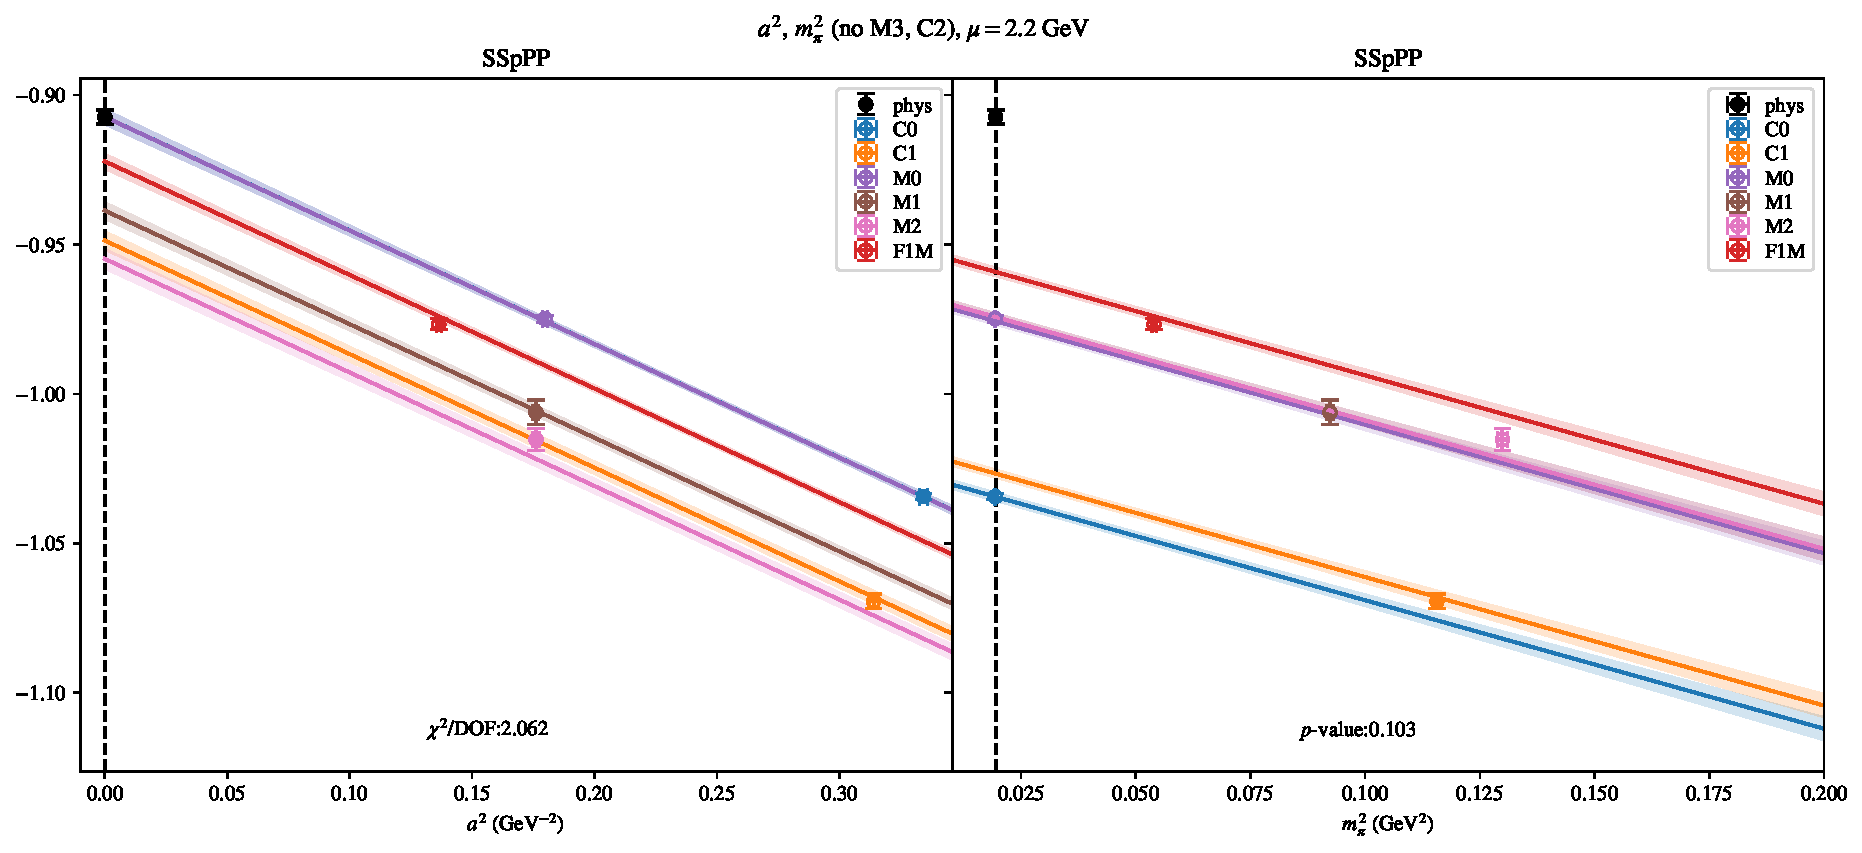
\includepdf[link, pages=-]{VVmAA/SUSY/bag_a2m2mcut_22.pdf}
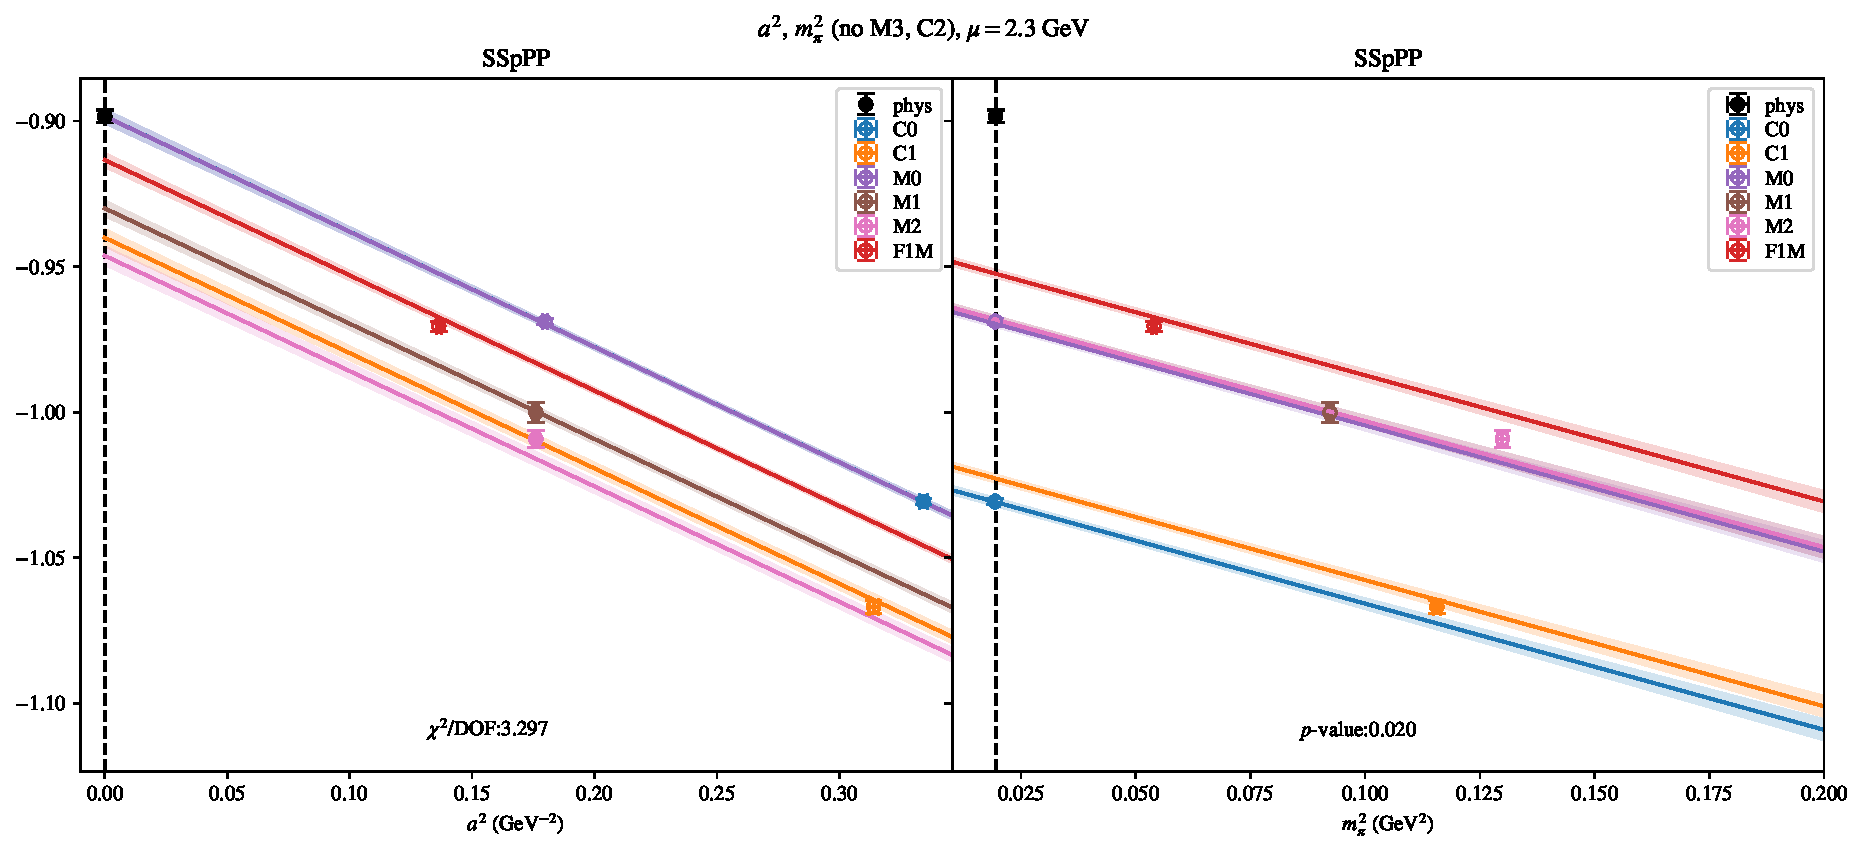
\includepdf[link, pages=-]{VVmAA/SUSY/bag_a2m2mcut_23.pdf}
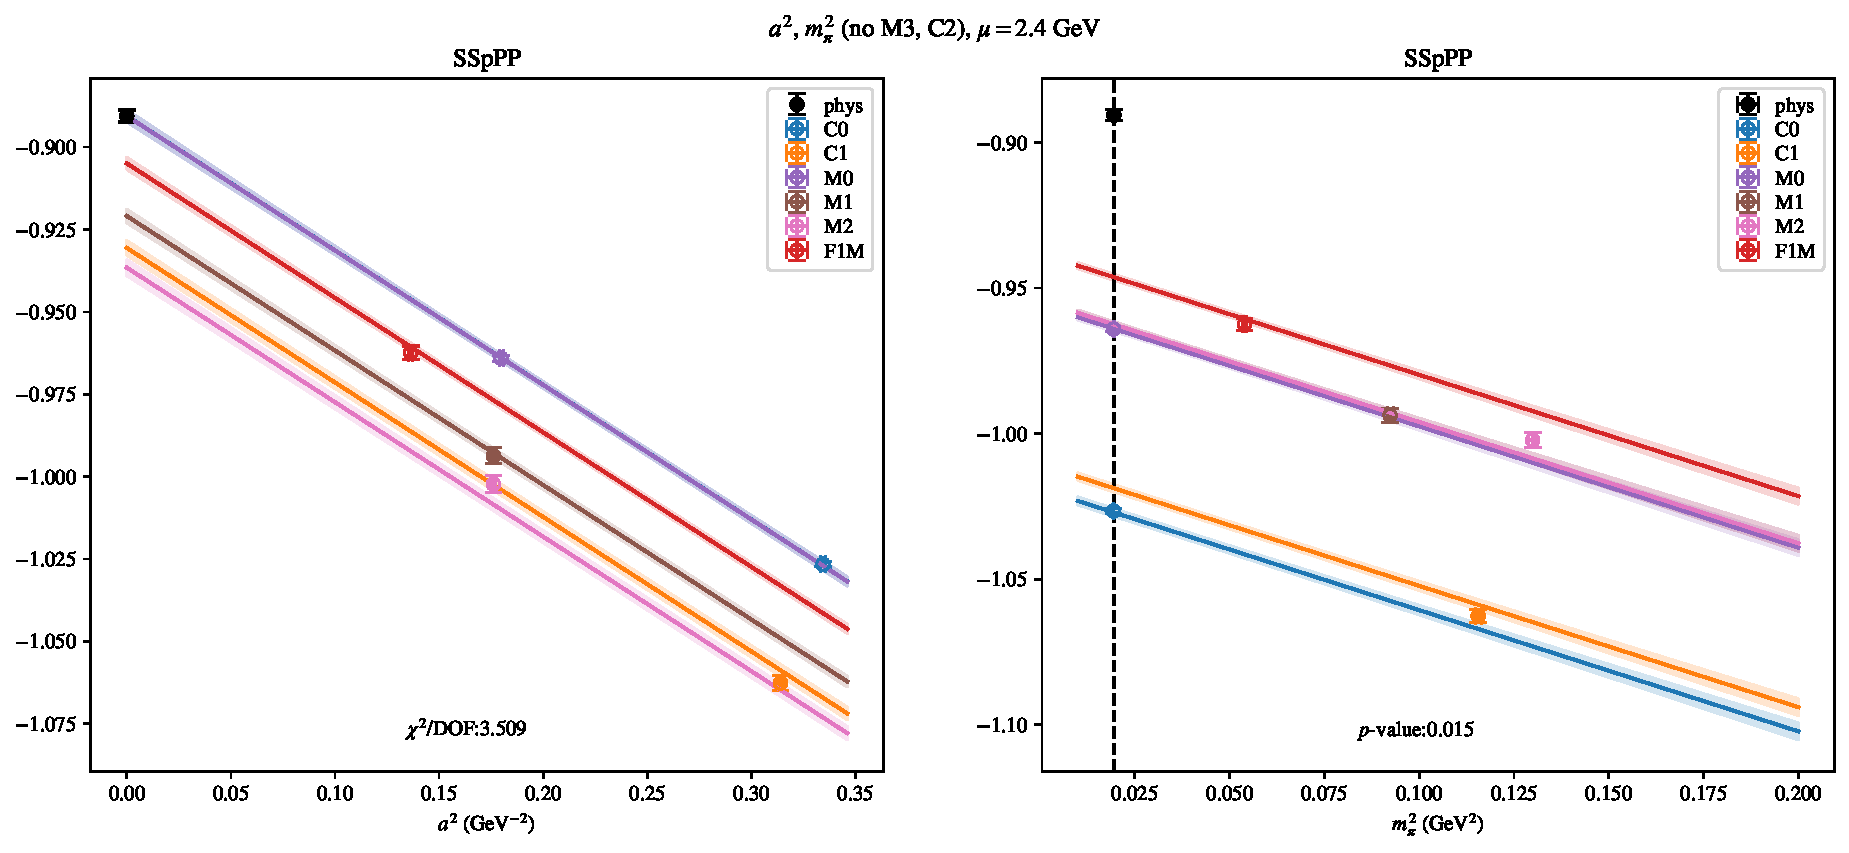
\includepdf[link, pages=-]{VVmAA/SUSY/bag_a2m2mcut_24.pdf}
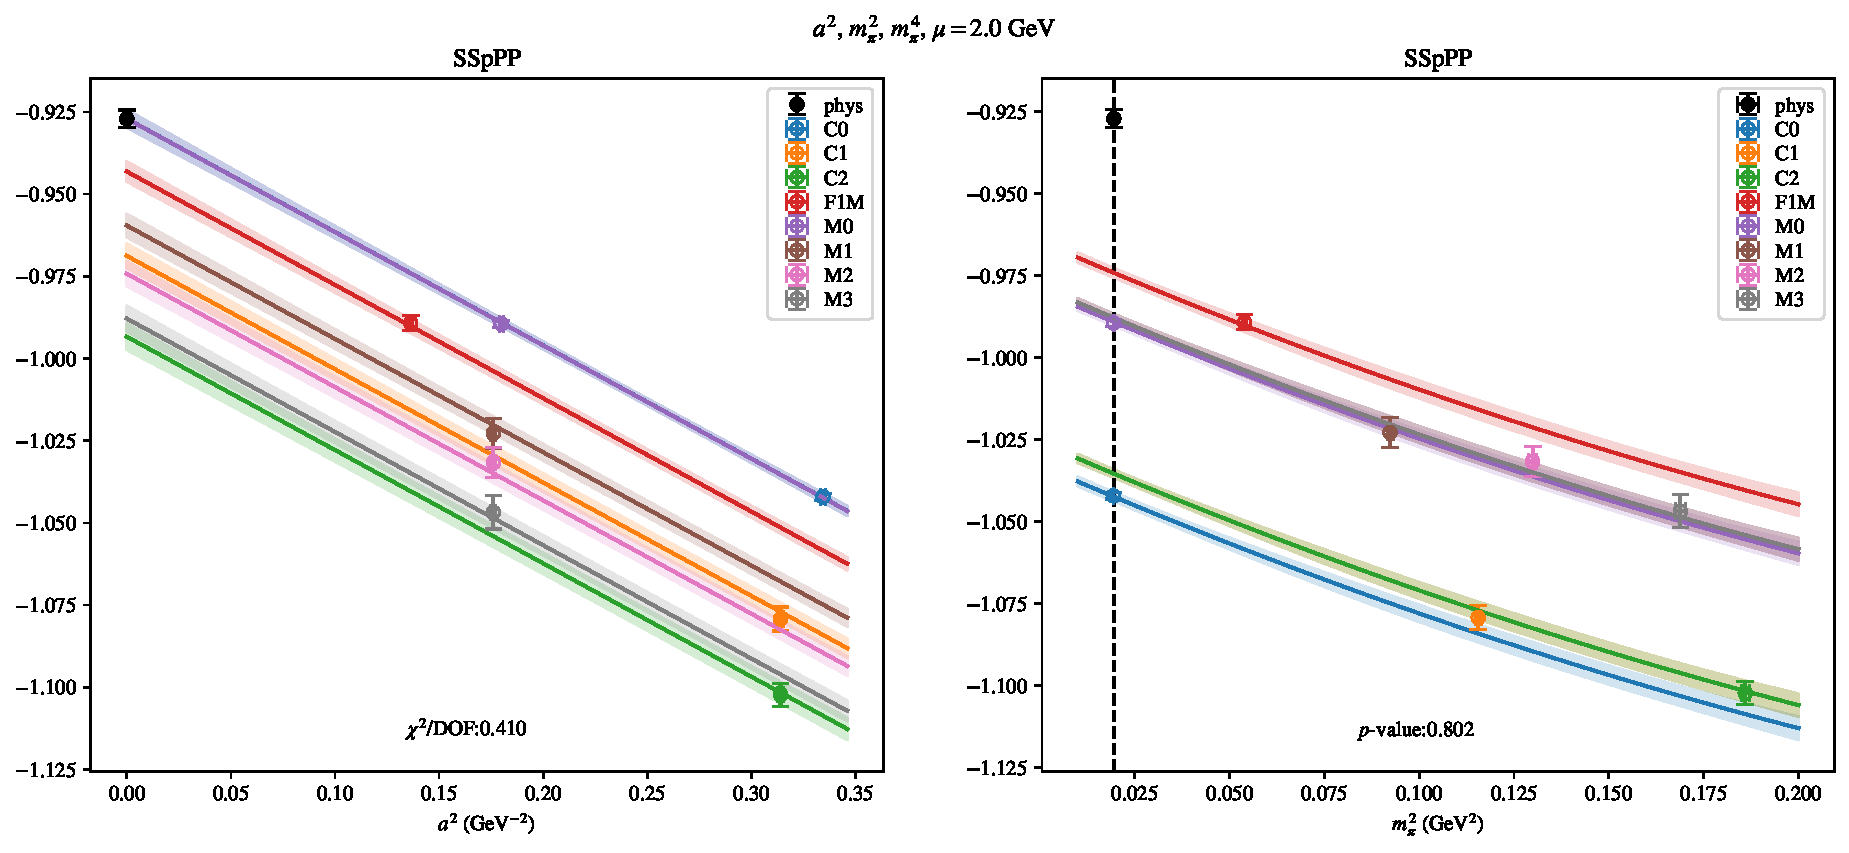
\includepdf[link, pages=-]{VVmAA/SUSY/bag_a2m2m4_20.pdf}
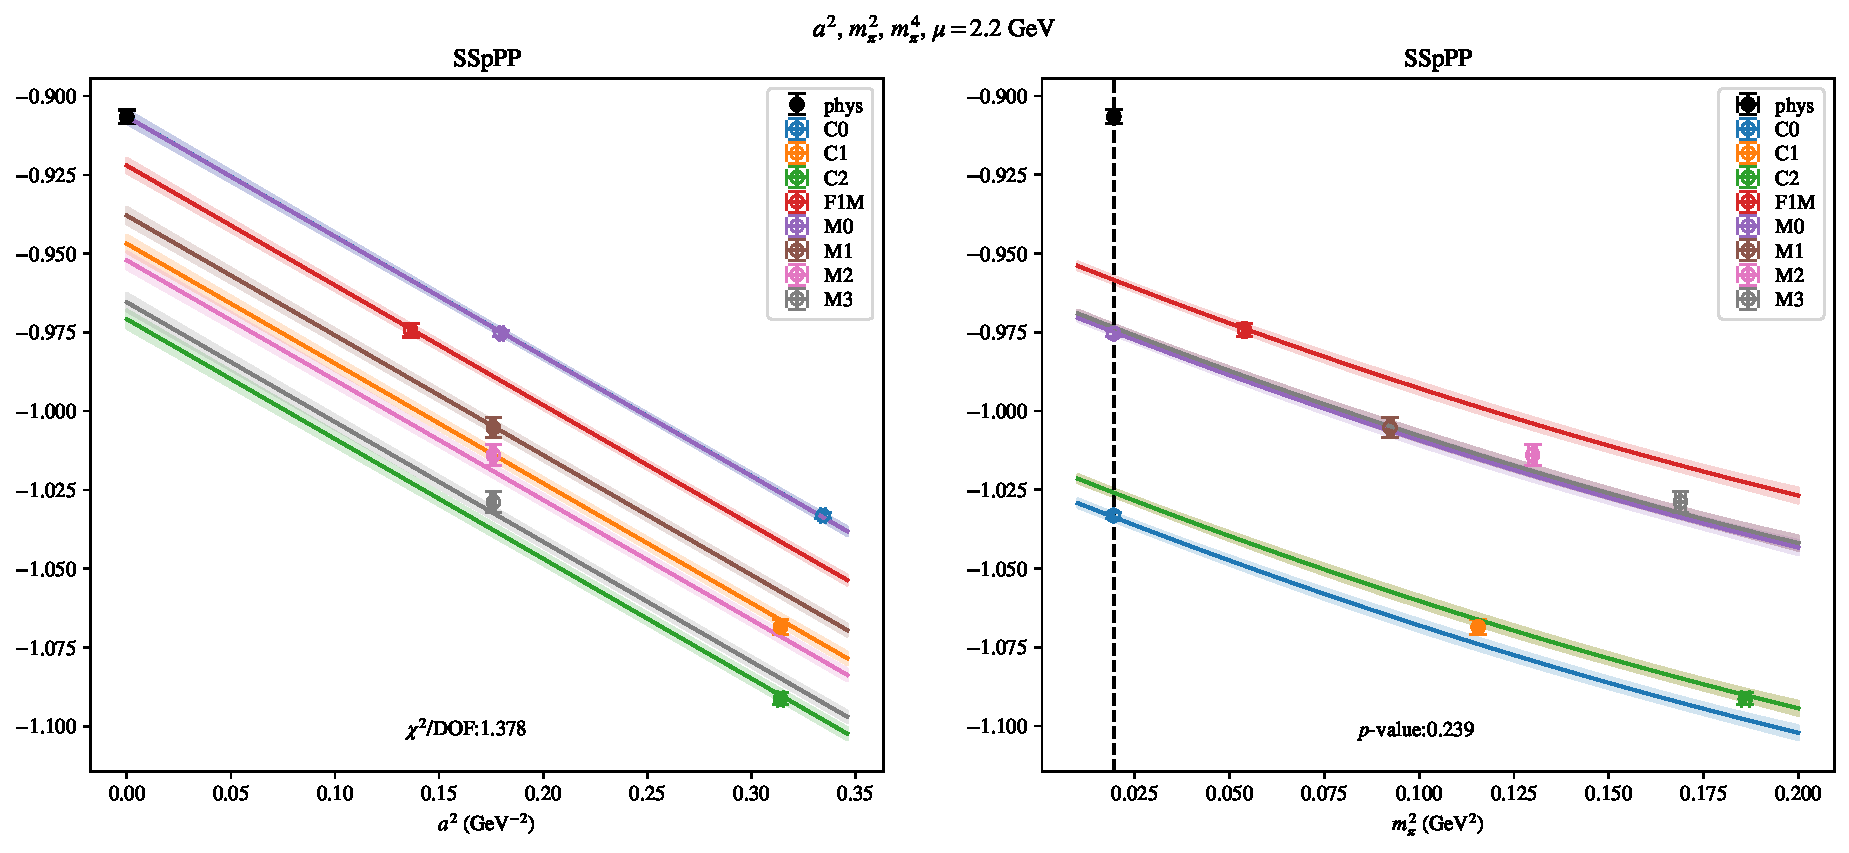
\includepdf[link, pages=-]{VVmAA/SUSY/bag_a2m2m4_22.pdf}
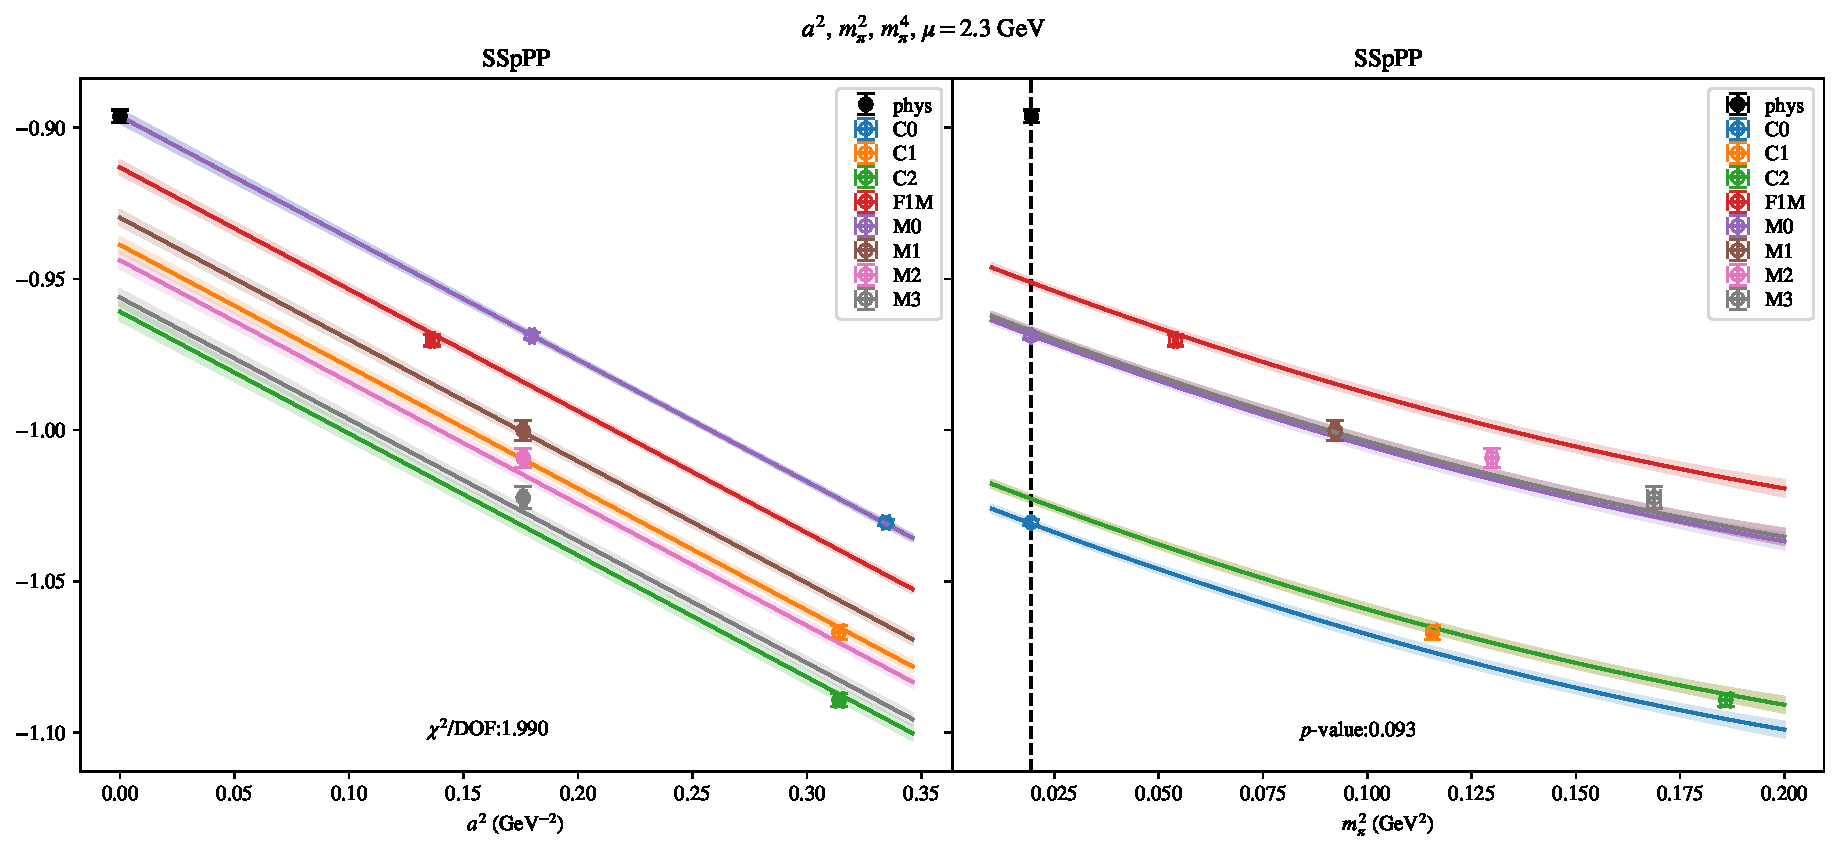
\includepdf[link, pages=-]{VVmAA/SUSY/bag_a2m2m4_23.pdf}
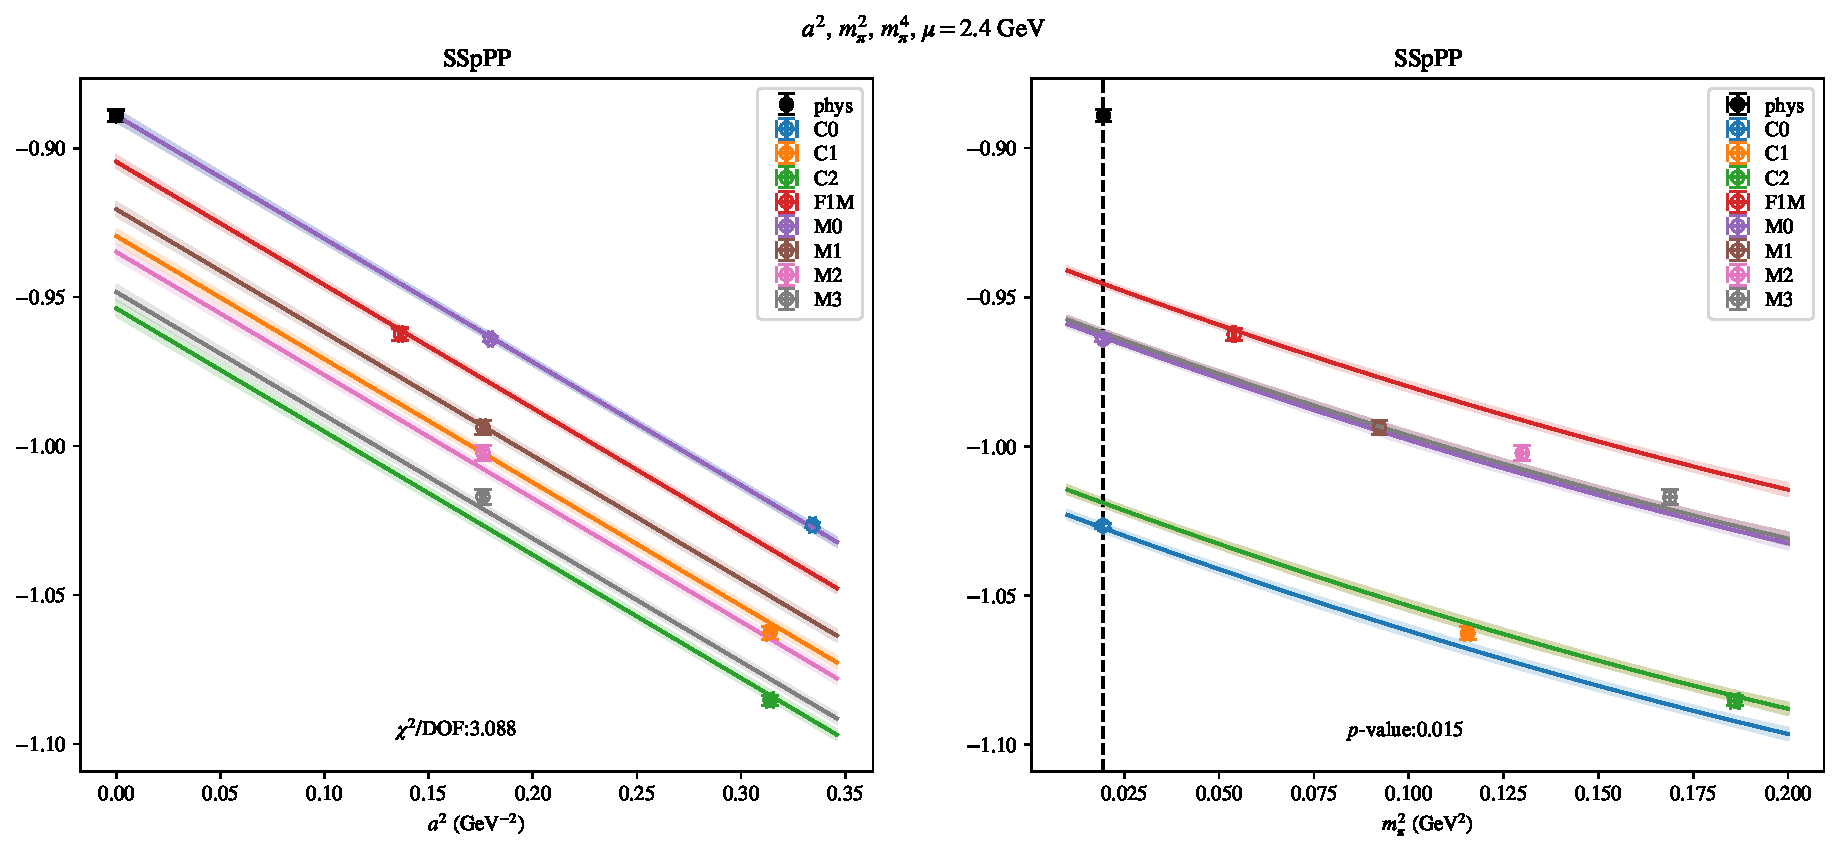
\includepdf[link, pages=-]{VVmAA/SUSY/bag_a2m2m4_24.pdf}
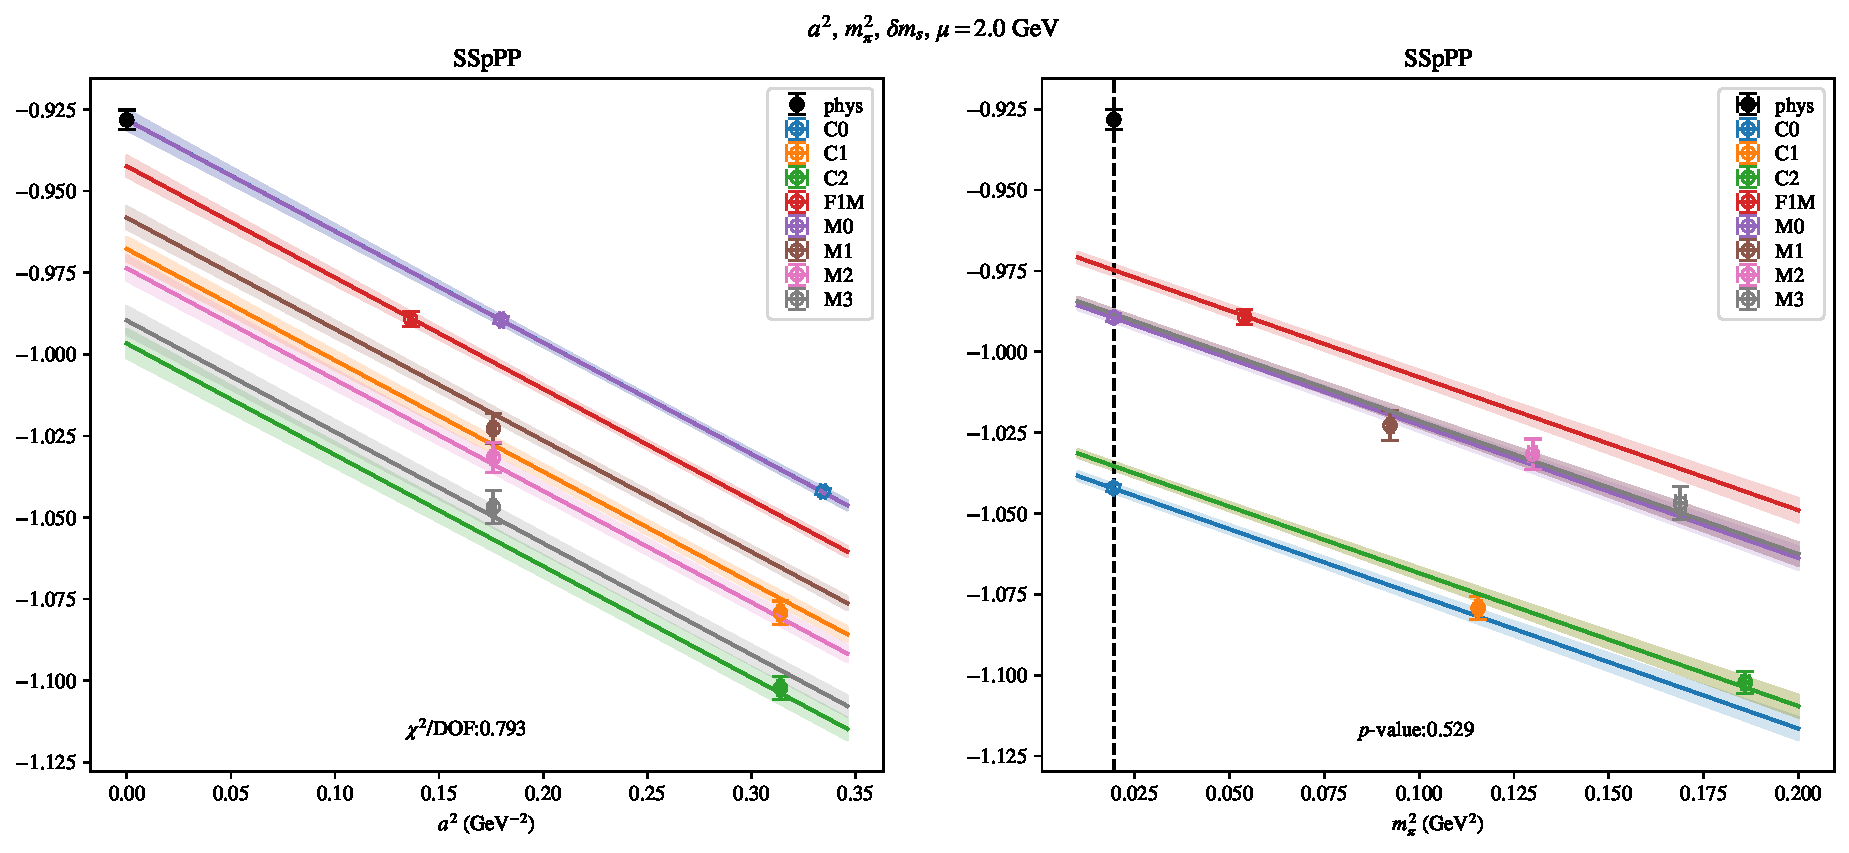
\includepdf[link, pages=-]{VVmAA/SUSY/bag_a2m2delm_20.pdf}
\includepdf[link, pages=-]{VVmAA/SUSY/bag_a2m2delm_22.pdf}
\includepdf[link, pages=-]{VVmAA/SUSY/bag_a2m2delm_23.pdf}
\includepdf[link, pages=-]{VVmAA/SUSY/bag_a2m2delm_24.pdf}
\clearpage
\section{$\mathcal{B}_3$}
\begin{table}[h!]
\begin{center}
\begin{tabular}{|c|c|c|c|c|c|c|}
\hline
$\mu$ (GeV) & $a^2$, $m_\pi^2$& $a^2$, $m_\pi^2$ (no C)& $a^2$, $m_\pi^2$, $a^4$& $a^2$, $m_\pi^2$ (no M3, C2)& $a^2$, $m_\pi^2$, $m_\pi^4$& $a^2$, $m_\pi^2$, $\delta m_s$\\
\hline
2.0& \hyperlink{SSmPP/SUSY/bag_a2m2_20.pdf.1}{\textbf{0.2814(22)}: 0.658 (0.655)} & \hyperlink{SSmPP/SUSY/bag_a2m2noC_20.pdf.1}{\textbf{0.288(10)}: 0.508 (0.601)} & \hyperlink{SSmPP/SUSY/bag_a2a4m2_20.pdf.1}{\textbf{0.283(17)}: 0.869 (0.481)} & \hyperlink{SSmPP/SUSY/bag_a2m2mcut_20.pdf.1}{\textbf{0.2811(25)}: 0.619 (0.602)} & \hyperlink{SSmPP/SUSY/bag_a2m2m4_20.pdf.1}{\textbf{0.2799(25)}: 0.444 (0.777)} & \hyperlink{SSmPP/SUSY/bag_a2m2delm_20.pdf.1}{\textbf{0.2813(22)}: 0.709 (0.586)}\\
2.2& \hyperlink{SSmPP/SUSY/bag_a2m2_22.pdf.1}{\textbf{0.2725(19)}: 1.054 (0.384)} & \hyperlink{SSmPP/SUSY/bag_a2m2noC_22.pdf.1}{\textbf{0.2810(88)}: 0.515 (0.597)} & \hyperlink{SSmPP/SUSY/bag_a2a4m2_22.pdf.1}{\textbf{0.275(14)}: 1.323 (0.258)} & \hyperlink{SSmPP/SUSY/bag_a2m2mcut_22.pdf.1}{\textbf{0.2727(21)}: 0.893 (0.444)} & \hyperlink{SSmPP/SUSY/bag_a2m2m4_22.pdf.1}{\textbf{0.2712(22)}: 0.763 (0.549)} & \hyperlink{SSmPP/SUSY/bag_a2m2delm_22.pdf.1}{\textbf{0.2725(20)}: 1.15 (0.331)}\\
2.3& \hyperlink{SSmPP/SUSY/bag_a2m2_23.pdf.1}{\textbf{0.2688(18)}: 1.32 (0.252)} & \hyperlink{SSmPP/SUSY/bag_a2m2noC_23.pdf.1}{\textbf{0.2782(79)}: 0.516 (0.597)} & \hyperlink{SSmPP/SUSY/bag_a2a4m2_23.pdf.1}{\textbf{0.273(13)}: 1.662 (0.156)} & \hyperlink{SSmPP/SUSY/bag_a2m2mcut_23.pdf.1}{\textbf{0.2687(20)}: 1.221 (0.3)} & \hyperlink{SSmPP/SUSY/bag_a2m2m4_23.pdf.1}{\textbf{0.2676(19)}: 1.004 (0.404)} & \hyperlink{SSmPP/SUSY/bag_a2m2delm_23.pdf.1}{\textbf{0.2687(18)}: 1.512 (0.196)}\\
2.4& \hyperlink{SSmPP/SUSY/bag_a2m2_24.pdf.1}{\textbf{0.2653(17)}: 1.742 (0.121)} & \hyperlink{SSmPP/SUSY/bag_a2m2noC_24.pdf.1}{\textbf{0.2751(74)}: 0.643 (0.526)} & \hyperlink{SSmPP/SUSY/bag_a2a4m2_24.pdf.1}{\textbf{0.270(12)}: 2.132 (0.074)} & \hyperlink{SSmPP/SUSY/bag_a2m2mcut_24.pdf.1}{\textbf{0.2653(18)}: 1.625 (0.181)} & \hyperlink{SSmPP/SUSY/bag_a2m2m4_24.pdf.1}{\textbf{0.2639(19)}: 1.347 (0.25)} & \hyperlink{SSmPP/SUSY/bag_a2m2delm_24.pdf.1}{\textbf{0.2652(17)}: 1.914 (0.105)}\\
\hline
\end{tabular}
\caption{Physical point value from chiral and continuum extrapolation at renormalisation scale $\mu$. Entries are \textbf{value(error)}: $\chi^2/\text{DOF}$ ($p$-value).}
\end{center}
\end{table}
\begin{table}[h!]
\begin{center}
\begin{tabular}{|c c|c|c|c|c|c|c|}
\hline
$\mu$ (GeV) &  & $a^2$, $m_\pi^2$& $a^2$, $m_\pi^2$ (no C)& $a^2$, $m_\pi^2$, $a^4$& $a^2$, $m_\pi^2$ (no M3, C2)& $a^2$, $m_\pi^2$, $m_\pi^4$& $a^2$, $m_\pi^2$, $\delta m_s$\\
\hline
\multirow{3}{0.5in}{2.0} & $\alpha$ & 0.1827(80)& 0.145(58)& 0.17(15)& 0.1830(89)& 0.1870(86)& 0.1824(78)\\
 & $\beta$ & 0.00198(14)& 0.00179(31)& 0.00199(17)& 0.00221(26)& 0.00299(80)& 0.00174(34)\\
 & $\gamma$ &  &  & 0.04(32)&  & -0.000090(69)& 0.009(12)\\
\hline
\multirow{3}{0.5in}{2.2} & $\alpha$ & 0.2088(68)& 0.163(52)& 0.18(13)& 0.2075(74)& 0.2125(74)& 0.2081(71)\\
 & $\beta$ & 0.00209(12)& 0.00184(25)& 0.00211(15)& 0.00233(22)& 0.00305(65)& 0.00187(29)\\
 & $\gamma$ &  &  & 0.05(26)&  & -0.000086(57)& 0.008(10)\\
\hline
\multirow{3}{0.5in}{2.3} & $\alpha$ & 0.2206(62)& 0.169(47)& 0.18(12)& 0.2200(70)& 0.2239(66)& 0.2201(65)\\
 & $\beta$ & 0.00210(13)& 0.00185(22)& 0.00213(13)& 0.00233(20)& 0.00312(61)& 0.00189(26)\\
 & $\gamma$ &  &  & 0.08(24)&  & -0.000091(53)& 0.0083(94)\\
\hline
\multirow{3}{0.5in}{2.4} & $\alpha$ & 0.2323(59)& 0.179(43)& 0.19(11)& 0.2313(64)& 0.2359(64)& 0.2318(59)\\
 & $\beta$ & 0.00213(11)& 0.00185(21)& 0.00216(12)& 0.00234(19)& 0.00312(59)& 0.00192(25)\\
 & $\gamma$ &  &  & 0.08(23)&  & -0.000088(52)& 0.0081(90)\\
\hline
\end{tabular}
\caption{Fit values of coefficients in $Q = Q_{phys} + \mathbf{\alpha} a^2 + \mathbf{\beta}\left(\frac{m_\pi^2}{f_\pi^2}-\frac{m_{\pi,PDG}^2}{f_\pi^2}\right) + \gamma(\ldots)$}
\end{center}
\end{table}
\includepdf[link, pages=-]{SSmPP/SUSY/bag_a2m2_20.pdf}
\includepdf[link, pages=-]{SSmPP/SUSY/bag_a2m2_22.pdf}
\includepdf[link, pages=-]{SSmPP/SUSY/bag_a2m2_23.pdf}
\includepdf[link, pages=-]{SSmPP/SUSY/bag_a2m2_24.pdf}
\includepdf[link, pages=-]{SSmPP/SUSY/bag_a2m2noC_20.pdf}
\includepdf[link, pages=-]{SSmPP/SUSY/bag_a2m2noC_22.pdf}
\includepdf[link, pages=-]{SSmPP/SUSY/bag_a2m2noC_23.pdf}
\includepdf[link, pages=-]{SSmPP/SUSY/bag_a2m2noC_24.pdf}
\includepdf[link, pages=-]{SSmPP/SUSY/bag_a2a4m2_20.pdf}
\includepdf[link, pages=-]{SSmPP/SUSY/bag_a2a4m2_22.pdf}
\includepdf[link, pages=-]{SSmPP/SUSY/bag_a2a4m2_23.pdf}
\includepdf[link, pages=-]{SSmPP/SUSY/bag_a2a4m2_24.pdf}
\includepdf[link, pages=-]{SSmPP/SUSY/bag_a2m2mcut_20.pdf}
\includepdf[link, pages=-]{SSmPP/SUSY/bag_a2m2mcut_22.pdf}
\includepdf[link, pages=-]{SSmPP/SUSY/bag_a2m2mcut_23.pdf}
\includepdf[link, pages=-]{SSmPP/SUSY/bag_a2m2mcut_24.pdf}
\includepdf[link, pages=-]{SSmPP/SUSY/bag_a2m2m4_20.pdf}
\includepdf[link, pages=-]{SSmPP/SUSY/bag_a2m2m4_22.pdf}
\includepdf[link, pages=-]{SSmPP/SUSY/bag_a2m2m4_23.pdf}
\includepdf[link, pages=-]{SSmPP/SUSY/bag_a2m2m4_24.pdf}
\includepdf[link, pages=-]{SSmPP/SUSY/bag_a2m2delm_20.pdf}
\includepdf[link, pages=-]{SSmPP/SUSY/bag_a2m2delm_22.pdf}
\includepdf[link, pages=-]{SSmPP/SUSY/bag_a2m2delm_23.pdf}
\includepdf[link, pages=-]{SSmPP/SUSY/bag_a2m2delm_24.pdf}
\clearpage
\section{$\mathcal{B}_4$}
\begin{table}[h!]
\begin{center}
\begin{tabular}{|c|c|c|c|c|c|c|}
\hline
$\mu$ (GeV) & $a^2$, $m_\pi^2$& $a^2$, $m_\pi^2$ (no C)& $a^2$, $m_\pi^2$, $a^4$& $a^2$, $m_\pi^2$ (no M3, C2)& $a^2$, $m_\pi^2$, $m_\pi^4$& $a^2$, $m_\pi^2$, $\delta m_s$\\
\hline
2.0& \hyperlink{SSpPP/SUSY/bag_a2m2_20.pdf.1}{\textbf{1.7941(31)}: 9.071 (0.0)} & \hyperlink{SSpPP/SUSY/bag_a2m2noC_20.pdf.1}{\textbf{1.706(14)}: 0.212 (0.809)} & \hyperlink{SSpPP/SUSY/bag_a2a4m2_20.pdf.1}{\textbf{1.647(23)}: 0.89 (0.469)} & \hyperlink{SSpPP/SUSY/bag_a2m2mcut_20.pdf.1}{\textbf{1.7948(35)}: 14.77 (0.0)} & \hyperlink{SSpPP/SUSY/bag_a2m2m4_20.pdf.1}{\textbf{1.7979(36)}: 9.999 (0.0)} & \hyperlink{SSpPP/SUSY/bag_a2m2delm_20.pdf.1}{\textbf{1.7933(31)}: 5.201 (0.0)}\\
2.2& \hyperlink{SSpPP/SUSY/bag_a2m2_22.pdf.1}{\textbf{1.7992(30)}: 8.163 (0.0)} & \hyperlink{SSpPP/SUSY/bag_a2m2noC_22.pdf.1}{\textbf{1.720(13)}: 0.189 (0.827)} & \hyperlink{SSpPP/SUSY/bag_a2a4m2_22.pdf.1}{\textbf{1.665(22)}: 1.034 (0.388)} & \hyperlink{SSpPP/SUSY/bag_a2m2mcut_22.pdf.1}{\textbf{1.8007(35)}: 13.028 (0.0)} & \hyperlink{SSpPP/SUSY/bag_a2m2m4_22.pdf.1}{\textbf{1.8038(35)}: 8.152 (0.0)} & \hyperlink{SSpPP/SUSY/bag_a2m2delm_22.pdf.1}{\textbf{1.7992(30)}: 6.085 (0.0)}\\
2.3& \hyperlink{SSpPP/SUSY/bag_a2m2_23.pdf.1}{\textbf{1.8017(30)}: 7.701 (0.0)} & \hyperlink{SSpPP/SUSY/bag_a2m2noC_23.pdf.1}{\textbf{1.725(13)}: 0.213 (0.808)} & \hyperlink{SSpPP/SUSY/bag_a2a4m2_23.pdf.1}{\textbf{1.672(22)}: 0.794 (0.529)} & \hyperlink{SSpPP/SUSY/bag_a2m2mcut_23.pdf.1}{\textbf{1.8027(34)}: 12.366 (0.0)} & \hyperlink{SSpPP/SUSY/bag_a2m2m4_23.pdf.1}{\textbf{1.8056(34)}: 7.894 (0.0)} & \hyperlink{SSpPP/SUSY/bag_a2m2delm_23.pdf.1}{\textbf{1.8014(30)}: 5.434 (0.0)}\\
2.4& \hyperlink{SSpPP/SUSY/bag_a2m2_24.pdf.1}{\textbf{1.8035(29)}: 7.108 (0.0)} & \hyperlink{SSpPP/SUSY/bag_a2m2noC_24.pdf.1}{\textbf{1.730(13)}: 0.196 (0.822)} & \hyperlink{SSpPP/SUSY/bag_a2a4m2_24.pdf.1}{\textbf{1.678(22)}: 0.756 (0.554)} & \hyperlink{SSpPP/SUSY/bag_a2m2mcut_24.pdf.1}{\textbf{1.8044(34)}: 11.566 (0.0)} & \hyperlink{SSpPP/SUSY/bag_a2m2m4_24.pdf.1}{\textbf{1.8071(34)}: 7.518 (0.0)} & \hyperlink{SSpPP/SUSY/bag_a2m2delm_24.pdf.1}{\textbf{1.8031(30)}: 5.005 (0.0)}\\
\hline
\end{tabular}
\caption{Physical point value from chiral and continuum extrapolation at renormalisation scale $\mu$. Entries are \textbf{value(error)}: $\chi^2/\text{DOF}$ ($p$-value).}
\end{center}
\end{table}
\begin{table}[h!]
\begin{center}
\begin{tabular}{|c c|c|c|c|c|c|c|}
\hline
$\mu$ (GeV) &  & $a^2$, $m_\pi^2$& $a^2$, $m_\pi^2$ (no C)& $a^2$, $m_\pi^2$, $a^4$& $a^2$, $m_\pi^2$ (no M3, C2)& $a^2$, $m_\pi^2$, $m_\pi^4$& $a^2$, $m_\pi^2$, $\delta m_s$\\
\hline
\multirow{3}{0.5in}{2.0} & $\alpha$ & 0.141(11)& 0.669(82)& 1.49(21)& 0.139(12)& 0.130(12)& 0.136(11)\\
 & $\beta$ & -0.00150(24)& -0.00171(57)& -0.00217(29)& -0.00179(42)& -0.0048(13)& -0.00406(60)\\
 & $\gamma$ &  &  & -2.74(43)&  & 0.00030(11)& 0.101(19)\\
\hline
\multirow{3}{0.5in}{2.2} & $\alpha$ & 0.153(11)& 0.631(78)& 1.39(20)& 0.149(12)& 0.139(12)& 0.147(11)\\
 & $\beta$ & -0.00093(23)& -0.00135(52)& -0.00158(27)& -0.00142(39)& -0.0045(11)& -0.00291(54)\\
 & $\gamma$ &  &  & -2.50(42)&  & 0.00032(10)& 0.077(18)\\
\hline
\multirow{3}{0.5in}{2.3} & $\alpha$ & 0.155(11)& 0.616(78)& 1.35(20)& 0.152(12)& 0.143(12)& 0.150(11)\\
 & $\beta$ & -0.00084(22)& -0.00124(51)& -0.00146(26)& -0.00120(38)& -0.0038(11)& -0.00277(53)\\
 & $\gamma$ &  &  & -2.43(42)&  & 0.00027(10)& 0.076(18)\\
\hline
\multirow{3}{0.5in}{2.4} & $\alpha$ & 0.157(10)& 0.602(77)& 1.31(20)& 0.154(12)& 0.146(12)& 0.152(11)\\
 & $\beta$ & -0.00076(22)& -0.00113(51)& -0.00136(26)& -0.00105(38)& -0.0035(11)& -0.00261(52)\\
 & $\gamma$ &  &  & -2.34(42)&  & 0.00025(10)& 0.073(18)\\
\hline
\end{tabular}
\caption{Fit values of coefficients in $Q = Q_{phys} + \mathbf{\alpha} a^2 + \mathbf{\beta}\left(\frac{m_\pi^2}{f_\pi^2}-\frac{m_{\pi,PDG}^2}{f_\pi^2}\right) + \gamma(\ldots)$}
\end{center}
\end{table}
\includepdf[link, pages=-]{SSpPP/SUSY/bag_a2m2_20.pdf}
\includepdf[link, pages=-]{SSpPP/SUSY/bag_a2m2_22.pdf}
\includepdf[link, pages=-]{SSpPP/SUSY/bag_a2m2_23.pdf}
\includepdf[link, pages=-]{SSpPP/SUSY/bag_a2m2_24.pdf}
\includepdf[link, pages=-]{SSpPP/SUSY/bag_a2m2noC_20.pdf}
\includepdf[link, pages=-]{SSpPP/SUSY/bag_a2m2noC_22.pdf}
\includepdf[link, pages=-]{SSpPP/SUSY/bag_a2m2noC_23.pdf}
\includepdf[link, pages=-]{SSpPP/SUSY/bag_a2m2noC_24.pdf}
\includepdf[link, pages=-]{SSpPP/SUSY/bag_a2a4m2_20.pdf}
\includepdf[link, pages=-]{SSpPP/SUSY/bag_a2a4m2_22.pdf}
\includepdf[link, pages=-]{SSpPP/SUSY/bag_a2a4m2_23.pdf}
\includepdf[link, pages=-]{SSpPP/SUSY/bag_a2a4m2_24.pdf}
\includepdf[link, pages=-]{SSpPP/SUSY/bag_a2m2mcut_20.pdf}
\includepdf[link, pages=-]{SSpPP/SUSY/bag_a2m2mcut_22.pdf}
\includepdf[link, pages=-]{SSpPP/SUSY/bag_a2m2mcut_23.pdf}
\includepdf[link, pages=-]{SSpPP/SUSY/bag_a2m2mcut_24.pdf}
\includepdf[link, pages=-]{SSpPP/SUSY/bag_a2m2m4_20.pdf}
\includepdf[link, pages=-]{SSpPP/SUSY/bag_a2m2m4_22.pdf}
\includepdf[link, pages=-]{SSpPP/SUSY/bag_a2m2m4_23.pdf}
\includepdf[link, pages=-]{SSpPP/SUSY/bag_a2m2m4_24.pdf}
\includepdf[link, pages=-]{SSpPP/SUSY/bag_a2m2delm_20.pdf}
\includepdf[link, pages=-]{SSpPP/SUSY/bag_a2m2delm_22.pdf}
\includepdf[link, pages=-]{SSpPP/SUSY/bag_a2m2delm_23.pdf}
\includepdf[link, pages=-]{SSpPP/SUSY/bag_a2m2delm_24.pdf}
\clearpage
\section{$\mathcal{B}_5$}
\begin{table}[h!]
\begin{center}
\begin{tabular}{|c|c|c|c|c|c|c|}
\hline
$\mu$ (GeV) & $a^2$, $m_\pi^2$& $a^2$, $m_\pi^2$ (no C)& $a^2$, $m_\pi^2$, $a^4$& $a^2$, $m_\pi^2$ (no M3, C2)& $a^2$, $m_\pi^2$, $m_\pi^4$& $a^2$, $m_\pi^2$, $\delta m_s$\\
\hline
2.0& \hyperlink{TT/SUSY/bag_a2m2_20.pdf.1}{\textbf{0.4932(39)}: 0.366 (0.872)} & \hyperlink{TT/SUSY/bag_a2m2noC_20.pdf.1}{\textbf{0.470(17)}: 0.098 (0.907)} & \hyperlink{TT/SUSY/bag_a2a4m2_20.pdf.1}{\textbf{0.458(28)}: 0.13 (0.971)} & \hyperlink{TT/SUSY/bag_a2m2mcut_20.pdf.1}{\textbf{0.4934(46)}: 0.586 (0.624)} & \hyperlink{TT/SUSY/bag_a2m2m4_20.pdf.1}{\textbf{0.4941(46)}: 0.416 (0.797)} & \hyperlink{TT/SUSY/bag_a2m2delm_20.pdf.1}{\textbf{0.4929(40)}: 0.352 (0.843)}\\
2.2& \hyperlink{TT/SUSY/bag_a2m2_22.pdf.1}{\textbf{0.5004(34)}: 0.36 (0.876)} & \hyperlink{TT/SUSY/bag_a2m2noC_22.pdf.1}{\textbf{0.480(15)}: 0.049 (0.952)} & \hyperlink{TT/SUSY/bag_a2a4m2_22.pdf.1}{\textbf{0.471(26)}: 0.158 (0.96)} & \hyperlink{TT/SUSY/bag_a2m2mcut_22.pdf.1}{\textbf{0.5006(40)}: 0.557 (0.643)} & \hyperlink{TT/SUSY/bag_a2m2m4_22.pdf.1}{\textbf{0.5011(37)}: 0.378 (0.824)} & \hyperlink{TT/SUSY/bag_a2m2delm_22.pdf.1}{\textbf{0.5002(34)}: 0.411 (0.801)}\\
2.3& \hyperlink{TT/SUSY/bag_a2m2_23.pdf.1}{\textbf{0.5036(32)}: 0.389 (0.857)} & \hyperlink{TT/SUSY/bag_a2m2noC_23.pdf.1}{\textbf{0.484(14)}: 0.049 (0.952)} & \hyperlink{TT/SUSY/bag_a2a4m2_23.pdf.1}{\textbf{0.473(23)}: 0.128 (0.972)} & \hyperlink{TT/SUSY/bag_a2m2mcut_23.pdf.1}{\textbf{0.5038(36)}: 0.613 (0.606)} & \hyperlink{TT/SUSY/bag_a2m2m4_23.pdf.1}{\textbf{0.5043(34)}: 0.443 (0.778)} & \hyperlink{TT/SUSY/bag_a2m2delm_23.pdf.1}{\textbf{0.5034(32)}: 0.42 (0.795)}\\
2.4& \hyperlink{TT/SUSY/bag_a2m2_24.pdf.1}{\textbf{0.5062(29)}: 0.429 (0.829)} & \hyperlink{TT/SUSY/bag_a2m2noC_24.pdf.1}{\textbf{0.487(13)}: 0.051 (0.95)} & \hyperlink{TT/SUSY/bag_a2a4m2_24.pdf.1}{\textbf{0.478(22)}: 0.163 (0.957)} & \hyperlink{TT/SUSY/bag_a2m2mcut_24.pdf.1}{\textbf{0.5063(33)}: 0.698 (0.553)} & \hyperlink{TT/SUSY/bag_a2m2m4_24.pdf.1}{\textbf{0.5071(32)}: 0.439 (0.781)} & \hyperlink{TT/SUSY/bag_a2m2delm_24.pdf.1}{\textbf{0.5060(28)}: 0.465 (0.761)}\\
\hline
\end{tabular}
\caption{Physical point value from chiral and continuum extrapolation at renormalisation scale $\mu$. Entries are \textbf{value(error)}: $\chi^2/\text{DOF}$ ($p$-value).}
\end{center}
\end{table}
\begin{table}[h!]
\begin{center}
\begin{tabular}{|c c|c|c|c|c|c|c|}
\hline
$\mu$ (GeV) &  & $a^2$, $m_\pi^2$& $a^2$, $m_\pi^2$ (no C)& $a^2$, $m_\pi^2$, $a^4$& $a^2$, $m_\pi^2$ (no M3, C2)& $a^2$, $m_\pi^2$, $m_\pi^4$& $a^2$, $m_\pi^2$, $\delta m_s$\\
\hline
\multirow{3}{0.5in}{2.0} & $\alpha$ & -0.084(13)& 0.05(10)& 0.24(26)& -0.085(15)& -0.086(15)& -0.085(14)\\
 & $\beta$ & 0.00073(26)& 0.00067(54)& 0.00054(29)& 0.00072(45)& 0.0003(13)& 0.00035(58)\\
 & $\gamma$ &  &  & -0.67(53)&  & 0.00004(11)& 0.015(21)\\
\hline
\multirow{3}{0.5in}{2.2} & $\alpha$ & -0.107(11)& 0.014(92)& 0.17(23)& -0.107(13)& -0.108(12)& -0.106(12)\\
 & $\beta$ & 0.00079(22)& 0.00069(45)& 0.00062(26)& 0.00068(38)& 0.0001(10)& 0.00057(50)\\
 & $\gamma$ &  &  & -0.56(48)&  & 0.000061(95)& 0.009(17)\\
\hline
\multirow{3}{0.5in}{2.3} & $\alpha$ & -0.119(11)& -0.0003(863)& 0.16(21)& -0.119(12)& -0.120(11)& -0.119(10)\\
 & $\beta$ & 0.00078(20)& 0.00069(41)& 0.00061(25)& 0.00070(36)& 0.00021(96)& 0.00053(48)\\
 & $\gamma$ &  &  & -0.57(43)&  & 0.000051(84)& 0.010(17)\\
\hline
\multirow{3}{0.5in}{2.4} & $\alpha$ & -0.130(10)& -0.017(76)& 0.13(20)& -0.130(11)& -0.132(10)& -0.1301(98)\\
 & $\beta$ & 0.00076(18)& 0.00070(38)& 0.00060(23)& 0.00070(33)& 0.00027(92)& 0.00052(41)\\
 & $\gamma$ &  &  & -0.52(42)&  & 0.000043(79)& 0.010(14)\\
\hline
\end{tabular}
\caption{Fit values of coefficients in $Q = Q_{phys} + \mathbf{\alpha} a^2 + \mathbf{\beta}\left(\frac{m_\pi^2}{f_\pi^2}-\frac{m_{\pi,PDG}^2}{f_\pi^2}\right) + \gamma(\ldots)$}
\end{center}
\end{table}
\includepdf[link, pages=-]{TT/SUSY/bag_a2m2_20.pdf}
\includepdf[link, pages=-]{TT/SUSY/bag_a2m2_22.pdf}
\includepdf[link, pages=-]{TT/SUSY/bag_a2m2_23.pdf}
\includepdf[link, pages=-]{TT/SUSY/bag_a2m2_24.pdf}
\includepdf[link, pages=-]{TT/SUSY/bag_a2m2noC_20.pdf}
\includepdf[link, pages=-]{TT/SUSY/bag_a2m2noC_22.pdf}
\includepdf[link, pages=-]{TT/SUSY/bag_a2m2noC_23.pdf}
\includepdf[link, pages=-]{TT/SUSY/bag_a2m2noC_24.pdf}
\includepdf[link, pages=-]{TT/SUSY/bag_a2a4m2_20.pdf}
\includepdf[link, pages=-]{TT/SUSY/bag_a2a4m2_22.pdf}
\includepdf[link, pages=-]{TT/SUSY/bag_a2a4m2_23.pdf}
\includepdf[link, pages=-]{TT/SUSY/bag_a2a4m2_24.pdf}
\includepdf[link, pages=-]{TT/SUSY/bag_a2m2mcut_20.pdf}
\includepdf[link, pages=-]{TT/SUSY/bag_a2m2mcut_22.pdf}
\includepdf[link, pages=-]{TT/SUSY/bag_a2m2mcut_23.pdf}
\includepdf[link, pages=-]{TT/SUSY/bag_a2m2mcut_24.pdf}
\includepdf[link, pages=-]{TT/SUSY/bag_a2m2m4_20.pdf}
\includepdf[link, pages=-]{TT/SUSY/bag_a2m2m4_22.pdf}
\includepdf[link, pages=-]{TT/SUSY/bag_a2m2m4_23.pdf}
\includepdf[link, pages=-]{TT/SUSY/bag_a2m2m4_24.pdf}
\includepdf[link, pages=-]{TT/SUSY/bag_a2m2delm_20.pdf}
\includepdf[link, pages=-]{TT/SUSY/bag_a2m2delm_22.pdf}
\includepdf[link, pages=-]{TT/SUSY/bag_a2m2delm_23.pdf}
\includepdf[link, pages=-]{TT/SUSY/bag_a2m2delm_24.pdf}
\clearpage
\end{document}